\documentclass[10pt, oneside]{book}
\usepackage[utf8]{inputenc}
\usepackage{amsmath}
\usepackage{amsthm}
\usepackage{amssymb}
\usepackage{enumitem}
\usepackage{mdframed}
\usepackage{hyperref}
\usepackage{multirow}
\usepackage{systeme}
%\usepackage{moresize}
\usepackage{relsize}
\usepackage{comment}
\usepackage{cancel}
\usepackage[a4paper,left=2.3cm, right=2.3cm, top=2.1cm, bottom=2.1cm]{geometry}
\usepackage[italian]{babel}
\usepackage{ragged2e}
\usepackage{fancyhdr}
\usepackage[Lenny]{fncychap}
%\ChTitleVar{\raggedleft\Huge\bfseries\fontfamily{cmss}\selectfont}
\usepackage{tikz}
\usepackage{pgfplots}
\usetikzlibrary{decorations.pathreplacing,calligraphy}
\usetikzlibrary { decorations.pathmorphing, decorations.shapes, }
\usepackage[cal=dutchcal]{mathalfa}
\usepackage{wrapfig}
\usepackage{physics}
\usepackage{listings}
\usepackage{graphicx}
\usepackage{eso-pic, transparent}
\usetikzlibrary{calc}
\usetikzlibrary{positioning}
\pgfplotsset{width=10cm,compat= newest}
\usepgfplotslibrary{external}
%\tikzexternalize
\usepackage{bbold}
\swapnumbers
\hypersetup{
    colorlinks=true,
    linkcolor=blue,
}
 
\renewcommand{\arraystretch}{1.3}
\setlength{\tabcolsep}{0.5cm}

\renewcommand{\qedsymbol}{\hfill \large $\blacksquare$}
%\renewcommand{\descriptionlabel}{$\ast$}
\newcommand{\celsius}{\, \mathrm{{}^\circ C}}
\newcommand{\evolt}{\, \mathrm{eV}}
\newcommand{\kelvin}[1]{\, \mathrm{K^{#1}}}
\newcommand{\joule}[1]{\, \mathrm{J^{#1}}}
\newcommand{\pascal}[1]{\, \mathrm{Pa^{#1}}}
\newcommand{\molvol}{\mathrm{v}}
\newcommand{\molms}{\mathcal{M}}
\newcommand{\angstrom}{\, \mathrm{\AA}}
\newcommand{\meters}[2]{\, \mathrm{#1 m^{#2}}}
\newcommand{\grams}[1]{\, \mathrm{g^{#1}}}
\newcommand{\mols}[1]{\, \mathrm{mol^{#1}}}
\newcommand{\limit}[2]{\lim\limits_{#1 \rightarrow #2}}
\newcommand{\deltas}[1]{\Delta S_{#1}}
\newcommand{\clausius}[2]{\frac{\delta Q_{#1}}{T_{#2}}}
\newcommand{\mean}[1]{\langle #1 \rangle}
\newcommand{\infobox}[2]{\vspace{0.5cm}~\\ \textbf{#1} \hrulefill \vspace{0.2cm}\\#2 {}\,\\\hrule \vspace{0.5cm}}
\newcommand{\lawbox}[2]{\begin{center}
\framebox{
\parbox{\linewidth}{
\vspace{0.3cm}
\textbf{#1} \hfill $\displaystyle #2$
\vspace{0.3cm}
}
}
\end{center}}

\newcommand{\lawboxtext}[2]{\begin{center}
\framebox{
\parbox{\linewidth}{
\vspace{0.3cm}
\textbf{#1} \vspace{0.1cm} \\#2
\vspace{0.3cm}
}
}
\end{center}}

\newcommand{\ds}{\displaystyle}
\newcommand{\tendsto}[2]{\xrightarrow[#1 \rightarrow #2]{}}
\newcommand{\integral}[4]{\int_{#1}^{#2} #3 \, \mathrm{d}#4}
\newcommand{\molhtv}{\mathcal{c}_V }
\newcommand{\molhtp}{\mathcal{c}_p }
\newcommand{\setel}[1]{ \{ #1\} }
\newcommand{\setprop}[3]{ \{ #1 \, \in \, #2 \, : \, #3 \}}
\def\upint{\mathchoice%
    {\mkern13mu\overline{\vphantom{\intop}\mkern7mu}\mkern-20mu}%
    {\mkern7mu\overline{\vphantom{\intop}\mkern7mu}\mkern-14mu}%
    {\mkern7mu\overline{\vphantom{\intop}\mkern7mu}\mkern-14mu}%
    {\mkern7mu\overline{\vphantom{\intop}\mkern7mu}\mkern-14mu}%
  \int}
\def\lowint{\mkern3mu\underline{\vphantom{\intop}\mkern7mu}\mkern-10mu\int}
%\def\derx{\frac{\textrm{d}^2}{\textrm{d}x^2}}

\title{SIOLI'S LECTURES ON THERMODYNAMICS}
\author{MAXIMILIANO SIOLI}
\date{a.a. 2022-2023}

\begin{document}
\makeatletter
\begin{titlepage}
\vspace{-2.1cm}
\AddToShipoutPictureBG*{%
  \AtPageLowerLeft{%
    \transparent{0.6}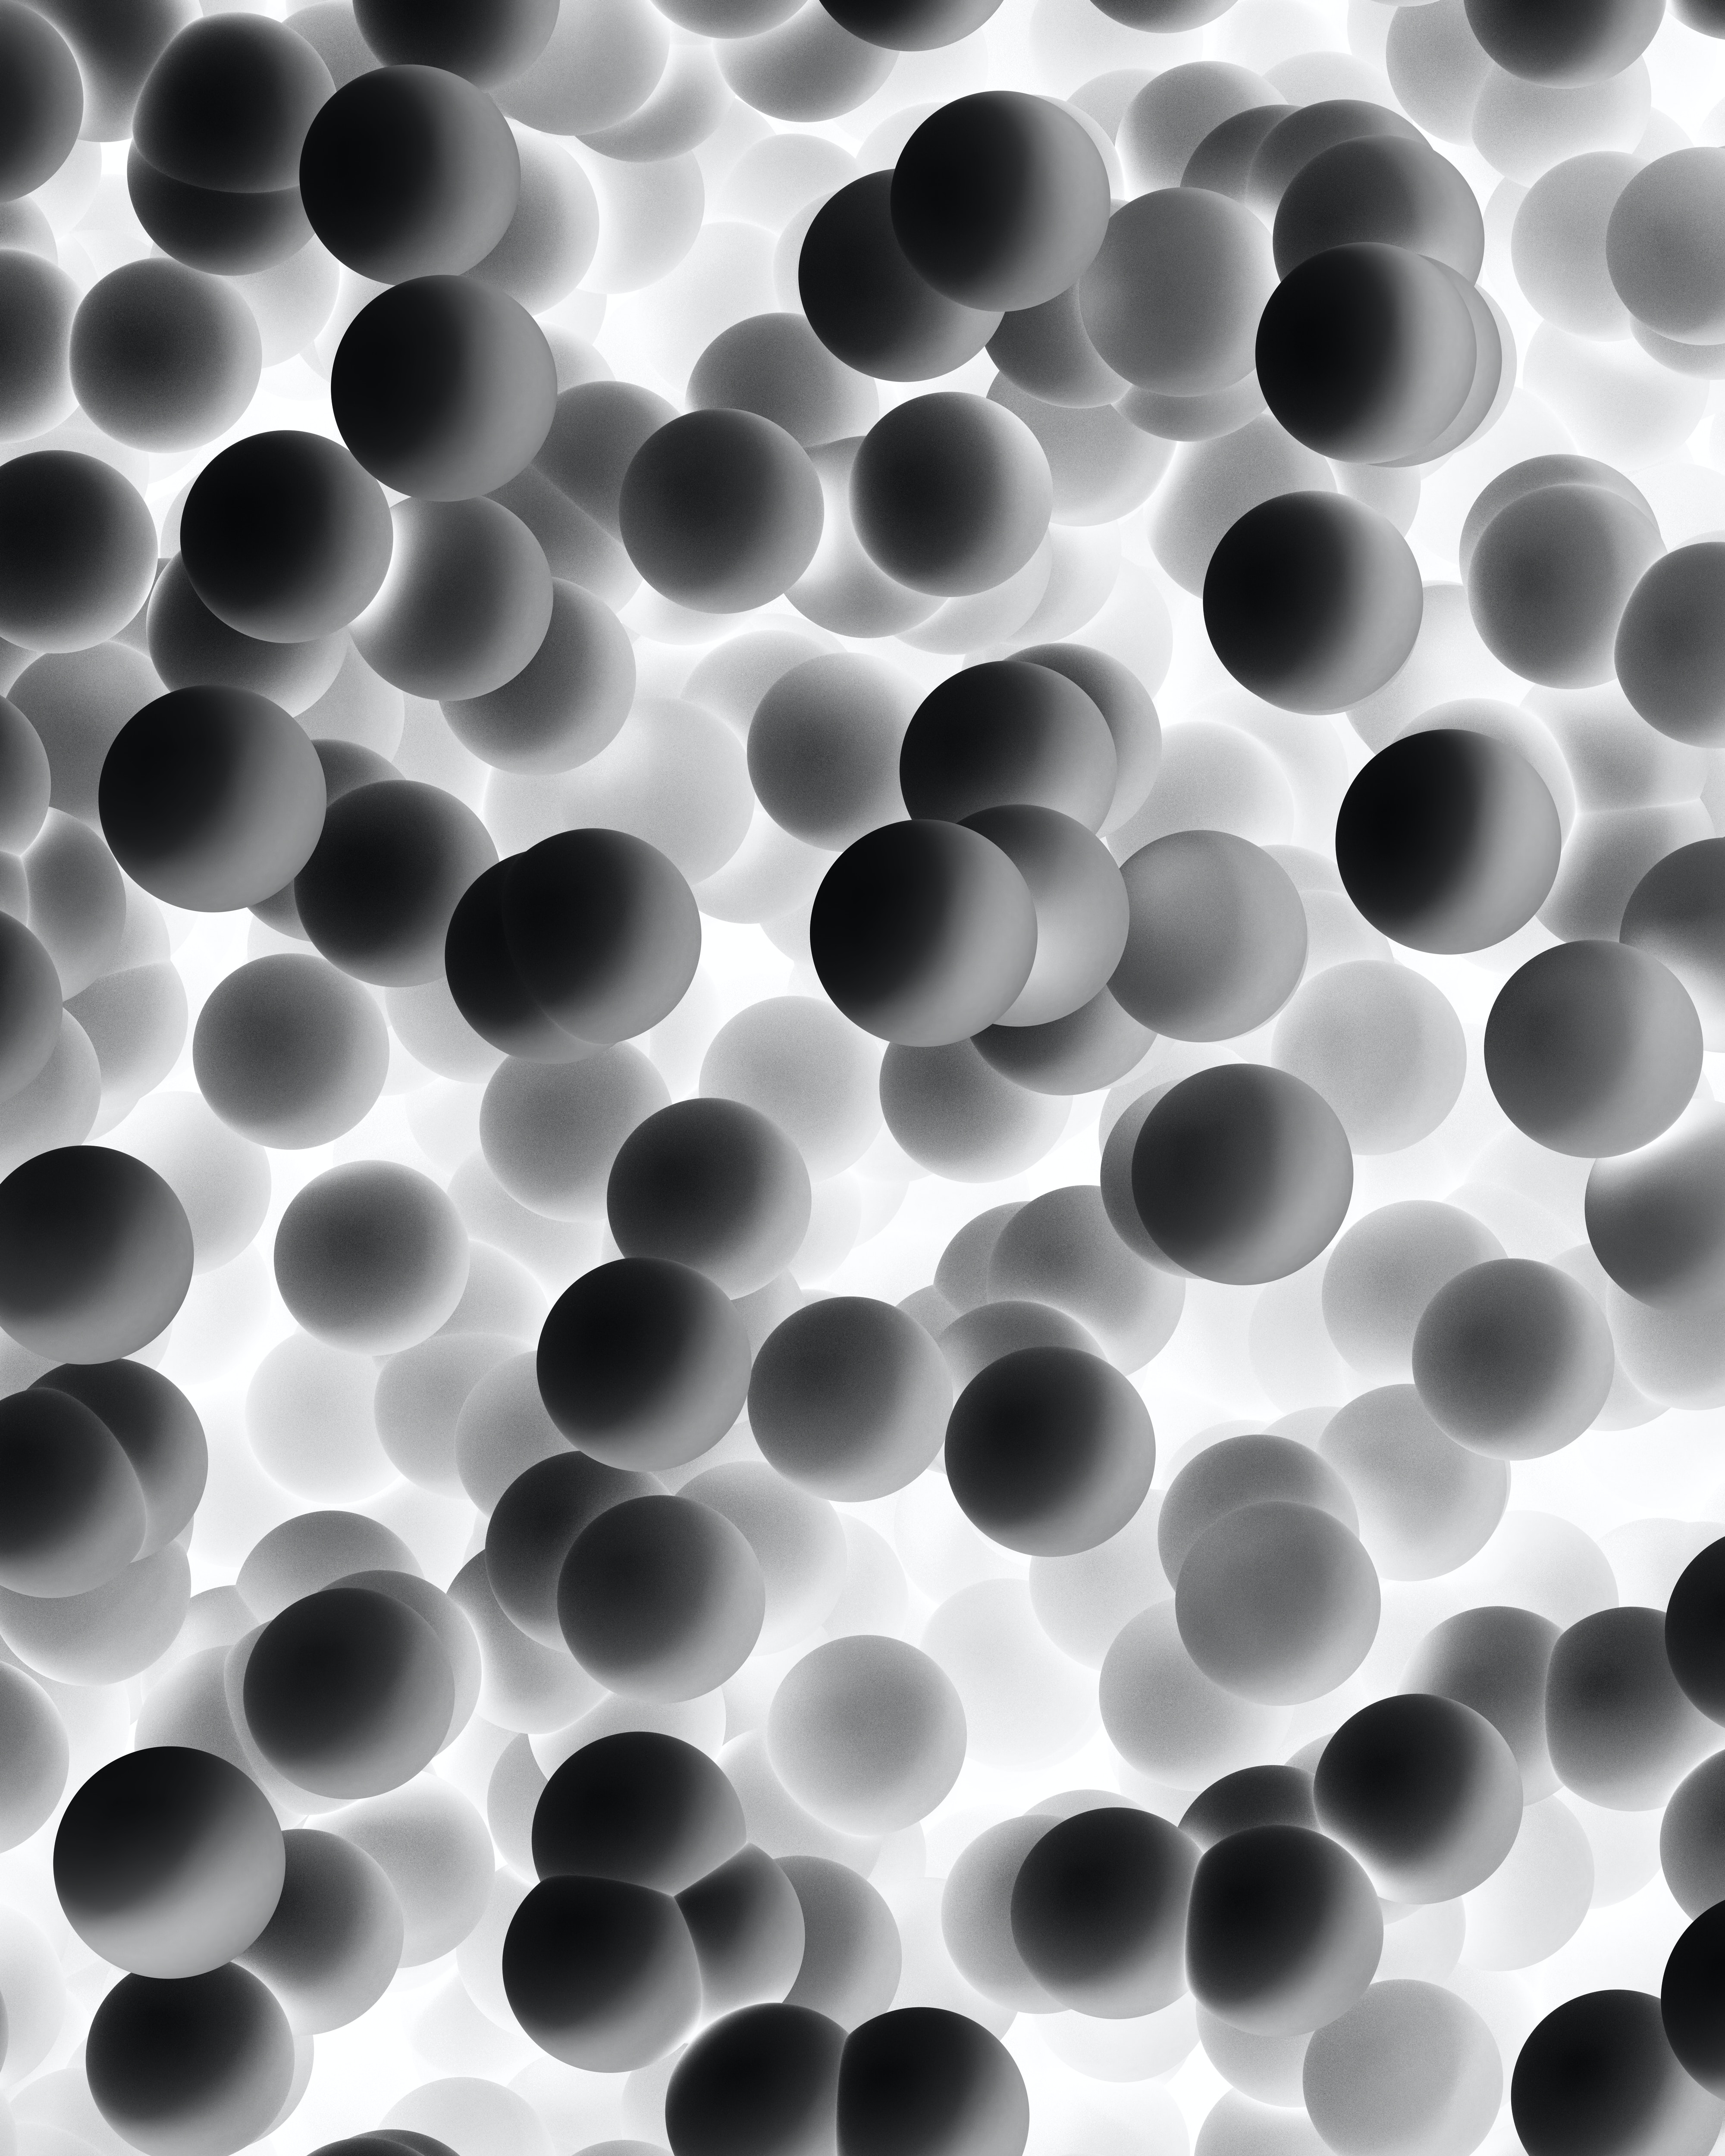
\includegraphics[width=\paperwidth,height=\paperheight]{cover.jpg}%
  }%
}
\hspace{0cm}
\vfill
\, \\\larger[20]\textsf{\textbf{SIOLI'S LECTURES \\ON THERMODYNAMICS}}
\\\smaller[2]MAXIMILIANO SIOLI
\\a.a. 2022-2023
\\~\\ \larger[20]\,\,
\\~\\ \,\,

\vfill
\hspace{0cm}
\end{titlepage}
\makeatother

\tableofcontents
\newpage

\chapter{Introduzione all'approccio termodinamico}
La \textbf{termodinamica classica} si occupa degli \textbf{scambi energetici} tra un \textbf{sistema fisico} e \textbf{l'ambiente circostante}. 
\begin{description}
\item[Sistema] porzione di spazio e/o di materia limitata.
\item[Ambiente] tutto ciò che è esterno al sistema ma può influenzarne il comportamento
\end{description}
Completa e generalizza la trattazione della meccanica classica a qualunque tipo di sistema o fenomeno fisico. \'E caratterizzata da:
\begin{description}
\item[Generalità]
\item[Immortalità] le sue leggi sono rimaste pressoché immutate nel progresso storico della scienza moderna (è valida infatti anche in ambito quantistico!). Si veda la citazione di Einstein:
\begin{quote}
Una teoria è tanto più convincente quanto più semplici sono le sue premesse, quanto più varie sono le cose che essa collega, quanto più esteso è il suo campo di applicazione. Per questo la termodinamica classica mi fece un'impressione così profonda. È la sola teoria fisica di contenuto universale che sono certo non sarà mai sovvertita, entro i limiti in cui i suoi concetti fondamentali sono applicabili (dedicato alla speciale attenzione di quelli che 
sono scettici per principio).
\end{quote}
\end{description}
Nasce dalla necessità dello studio di modalità di conversione del calore in lavoro (e quindi energia meccanica).
\\Lo studio della relazione tra sistema e ambiente (ovvero altri sistemi) si traduce nella descrizione quantitativa del comportamento del sistema e delle sue interazioni. Esistono due approcci: uno macroscopico, proprio della termodinamica \textit{classica}, che prescinde dalla descrizione dei costituenti elementari, e uno microscopico.

\subsection{Approccio microscopico}
Per un sistema di $N$ punti materiali, si definisce il \textbf{microstato (o stato microscopico)} secondo:
\begin{description}
\item[Microstato] insieme di quantità vettoriali che definiscono la descrizione dinamica di tutti i costituenti elementari (le particelle).
\end{description}
Si rappresenta come
\[\{\vec{x}_i, \vec{p}_i\}_{i = 1, ..., N}\]
Con i vettori posizione e i momenti. Ogni quantità vettoriale corrisponde, nello spazio tridimensionale, a tre scalari. Dunque in totale il microstato è un insieme di 6N quantità $\displaystyle \in \, \mathbb{R}$.
\\Noto lo stato del sistema ad un dato istante nel tempo e il campo di forze cui è sottoposto, è possibile studiarne l'evoluzione dinamica nel tempo, impostando un sistema di 3N equazioni differenziali del II ordine scalari (applicando Newton). Si nota che poiché nella II Legge della dinamica compare la derivata seconda della posizione, le leggi della dinamica classica sono \textbf{invarianti per inversione temporale}: si può studiare l'evoluzione sia nel futuro che nel passato.
\[\begin{cases}
m_1 \ddot{ \vec{x}}_1 = \vec{f}_1 = \vec{f}_1^{(e)} + \sum\limits_{i=2}^N \vec{f}_{1i}\\
\quad \vdots\\
m_N \ddot{ \vec{x}}_N = \vec{f}_N = \vec{f}_N^{(e)} + \sum\limits_{i=1}^{N-1} \vec{f}_{Ni}
\end{cases}\]
considerando forze interne ed esterne. La risoluzione richiede $2 \cdot 3N = 6N$ condizioni al contorno scalari, e conduce all'equazione oraria del moto delle particelle.
\\Essa può essere rappresentata come una curva nello \textbf{Spazio delle fasi (o degli stati)}
\begin{description}
\item[Spazio delle fasi] Spazio matematico astratto $6N$-dimensionale i cui punti rappresentano ogni possibile microstato del sistema.
\end{description}
Esiste un vincolo sulla grandezza di $N$? In linea di principio, secondo il determinismo assoluto (classico) incarnato dal \textbf{Demone di Laplace} il problema del moto è sempre risolvibile per qualsiasi numero di particelle: un'intelligenza in grado di conoscere perfettamente lo stato ed il campo di forze può anche conoscere esattamente lo sviluppo passato e futuro.
\\In pratica, tuttavia, $N \sim N_A = 6 \cdot 10^{23}$ per sistemi normalmente studiati e $N \sim 10^{80}$ per l'universo osservabile: risulta di fatto impossibile, anche solo con metodi numerici che consentano un margine d'errore accettabile, risolvere il sistema di differenziali.
\paragraph{Crisi del determinismo laplaciano} nel '900 il determinismo classico è stato poi minato da 
\begin{description}
\item[Teoria del caos] una minima (ma inevitabile) incertezza sperimentale di misura sulle condizioni al contorno tende a propagarsi, generando un cono di incertezza con crescita esponenziale, tramite dispersione e amplificazione. Dopo un certo tempo si ha una perdita di informazione sul microstato tanto importante da rendere inutili le previsioni
\item[Principio di indeterminazione di Heisenberg] la descrizione meccanica delle singole particelle è probabilistica: è impossibile conoscere con eguale precisione posizione e momento secondo
\[\Delta x \Delta p \geq \hbar\]
\end{description}
\paragraph{La Dinamica dei sistemi} rappresenta un possibile approccio risolutivo: con le equazioni cardinali si sacrifica la conoscenza esatta del microstato per inglobare l'informazione in pochi parametri rappresentativi dell'intero sistema
\[\begin{cases}
\sum \vec{f_i}^{(e)} = \dot{ \vec{P}} = M \dot{ \vec{v}}_{CM}\\
\sum \vec{\mathcal{M}_i}^{(e)} = \dot{ \vec{L}}_\Omega = \dv[•]{•}{t} \big(\vec{L}_{CM} + \vec{r}_{CM} \times \vec{P}\big)\\
\end{cases}\]
Per $N < 3$ il sistema impostato è risolvibile analiticamente (le due equazioni cardinali vettoriali, e quindi corrispondenti 6 scalari, del I ordine sono sufficienti fino a $3N = 6$, ovvero $N=2$ d.o.f.): per ordini di grandezza maggiori è necessaria l'imposizione di vincoli che contengano il numero di gradi di libertà. Si ha il corpo rigido
\begin{description}
\item[Corpo rigido] un sistema di punti materiali le cui distanze reciproche sono fisse.
\end{description}
Si noti che esso è un costrutto puramente matematico, non esiste nella realtà (l'azione istantanea a distanza per mantenere la perfetta rigidità viola la località relativistica). Il numero dei suoi gradi di libertà è mantenuto costante a $6$, corrispondenti a
\begin{description}
\item 3 per la posizione del centro di massa +
\item 3 per gli angoli di Eulero. Questi descrivono l'orientazione relativa di una terna ortogonale propria del corpo, definita fissando 3 punti ed il CM, rispetto a una terna fissa in un SdR inerziale.
\end{description}
Un altro possibile approccio è quello di uno dei due rami della trattazione termodinamica.
\paragraph{La termodinamica statistica} si basa sulla conoscenza di opportuni valori medi di grandezze microscopiche reinterpretabili in termini macroscopici, ovvero in termini di fenomeni e proprietà emergenti. Poiché le forze in gioco nella trattazione sono tendenzialmente la gravità e l'elettromagnetismo, essa è applicabile fino a energie $\sim 10^{9} \, \mathrm{eV}$. 
\\Essa è efficace sotto l'assunto di fluttuazioni contenute. Ipotizzando un regime poissoniano per l'incertezza, si ha
\[\frac{\delta N}{N} \sim \frac{1}{\sqrt{N}} \xrightarrow[N \rightarrow +\infty]{} 0\]
dunque la trattazione è valida per $N$ elevati. In genere il limite del campo di applicabilità dipende dal modello specifico.

\section{Approccio macroscopico: la termodinamica classica}
La termodinamica classica descrive un \textbf{sistema termodinamico} tramite il suo \textbf{macrostato}, caratterizzato da \textbf{coordinate termodinamiche macroscopiche} (pressione, volume, densità, composizione chimica, etc.) indipendenti dal tempo.
\begin{description}
\item[Sistema termodinamico] un sistema fisico descrivibile attraverso coordinate termodinamiche.
\end{description}
Le c.t. possono essere
\begin{description}
\item[Estensive] ovvero avere proprietà di \textbf{additività} (variano con la quantità di materia nel sistema)
\item[Intensive] ovvero \textbf{non} essere additive
\end{description}
Tra i due tipi vi sono relazioni peculiari: si possono infatti determinare \textbf{coppie di variabili coniugate} $(int, \, est)$
\paragraph{Il prototipo di sistema studiato nel corso} è un \textbf{sistema idrostatico} costituito da un gas in un cilindro con un pistone.
\begin{description}
\item[Sistema idrostatico] sistema termodinamico che esercita una pressione uniforme nei confronti dell'ambiente
\end{description}
All'equilibrio esso è un esempio di \textbf{sistema semplice}.
\begin{description}
\item[Sistema semplice] un sistema termodinamico completamente descrivibile a livello macroscopico tramite 3 c.t., di cui due indipendenti. Definito 'sistema XYZ' da Zemansky.
\end{description}
\subsection{Equilibrio termodinamico}
Si definisce secondo
\begin{description}
\item[Equilibrio termodinamico] stato di un sistema termodinamico tale per cui le coordinate termodinamiche rimangono immutate nel tempo (a meno di fluttuazioni statistiche)
\end{description}
Si osserva che fuori dall'equilibrio in realtà le c.t. non hanno valori uniformi all'interno del sistema (vi sono forti disomogeneità): esse infatti caratterizzano un sistema \textbf{solo all'equilibrio!}
\\L'oggetto di studio del corso è infatti la \textit{termodinamica assiomatica dei sistemi all'equilibrio} (vecchio nome), in quanto oltre a quanto detto si basa su assiomi di derivazione sperimentale. La termodinamica classica è quindi in qualche modo una 'termostatica'.
\paragraph{Si ha l'equilibrio termodinamico} quando sono verificati contemporaneamente:
\begin{description}
\item[Equilibrio meccanico] ovvero uno stato in cui non si hanno parti meccaniche in moto (considerando il sistema nel complesso, a livello macroscopico)
\item[Equilibrio chimico] ovvero le concentrazioni e la composizione non variano nel tempo
\item[Eq. termico] ovvero la temperatura del sistema si mantiene costante
\end{description}

Si definiscono quindi
\begin{description}
\item[Universo termodinamico] l'insieme del sistema e dell'ambiente circostante
\[U = S + A\]
\end{description}
\begin{center}

\begin{tabular}{c|c c}
& \multicolumn{2}{c}{Scambia}\\
& Materia & Energia\\\hline
Aperto & sì & sì\\
Chiuso & no & sì\\
Isolato & no & no

\end{tabular}

\end{center}
Si nota che la definizione del confine tra $S$ e $A$ per casi specifici presenta un qualche grado di arbitrarietà e può variare a seconda delle esigenze della trattazione.

\subsection{Gradi di libertà termodinamici}
Non tutte le c.t. sono necessarie per caratterizzare completamente lo stato di un sistema termodinamico all'equilibrio: sono sufficienti quelle indipendenti.
\begin{description}
\item[Grandezze indipendenti] possono assumere valori arbitrari
\item[Grandezze dipendenti] date due gr. $x$, $y$ indipendenti, una terza $z$ è dipendente se $\exists f'(x,y) = z$ o, alternativamente
\[\exists \, f \, : \, f(x,y,z) = 0\]
ovvero è possibile definire un'equazione di stato
\item[Equazione di stato] funzione delle c.t. di un sistema che ha valore costante ($0$) e dunque esprime un vincolo tra valori di queste.
\item[Gradi di libertà termodinamici] numero di c.t. \textbf{intensive} indipendenti di un sistema
\end{description}
Il numero di d.o.f. termodinamici è dato dalla 
\begin{center}

\framebox{
\parbox{\linewidth}{
\vspace{0.3cm}
\textbf{REGOLA DELLE FASI DI GIBBS} \hfill $\displaystyle \nu = C + 2 - F$
\vspace{0.3cm}
}
}
\end{center}
ove $C$ sono le componenti e $F$ le fasi.
\begin{description}
\item[Fase] regione di spazio (o di un sistema termodinamico) con proprietà uniformi della materia. Corrispondono agli stati di aggregazione di una sostanza.
\end{description}
$\nu$ può variare con l'energia (ovvero con la temperatura), in quanto a seconda del superamento di date soglie possono manifestarsi, oltre alla fase solida, in ordine: la fase liquida, quella aeriforme (le uniche altre trattate nel corso), il plasma ed il QGP, ovvero plasma di quark e gluoni. Le leggi della termodinamica classica sono universalmente applicabili a tutti gli stati di aggregazione (!).

\chapter{Principio Zero e Temperatura}
Si dimostra come il concetto di temperatura emerga spontaneamente da quello di equilibrio termico, tramite il \textbf{Principio Zero della Termodinamica}.
\\Siano dati due sistemi semplici $A$, $B$ con c.t. indipendenti $(x,y)$ e $(x',y')$ rispettivamente. Siano essi posti a contatto attraverso una \textbf{parete}.
\begin{description}
\item[Parete] superficie (reale o figurata) che delimita il sistema nello spazio metrico completo
\end{description}
Si definiscano quindi due tipi di pareti:
\begin{description}
\item[Adiabatica] se mantiene inalterate le coppie di c.t. dei due sistemi che la determinano
\item[Conduttrice (o diatermica)] se $\displaystyle \exists \, f(x,y; x', y') = 0$	 \\ovvero le coppie di c.t. si modificano in modo non indipendente
\end{description}
Si enuncia una prima definizione di equilibrio termico
\begin{quote}
Due sistemi a contatto attraverso una parete conduttrice sono all'equilibrio termico.
\\Equivalentemente, due sistemi si dicono all'equilibrio termico se sono in stati tali per cui se posti a contatto tramite una parete diatermica si avrebbe un sistema complessivo in equilibrio termico.
\end{quote}
Siano $A$, $B$ separati da parete adiabatica ma a contatto termico con un medesimo terzo sistema $C$, descritto da $(x'', y'')$. Si osserva un fondamentale fatto sperimentale, elevato al rango di principio:
\begin{center}

\framebox{
\parbox{\linewidth}{
\vspace{0.3cm}
\textbf{PRINCIPIO ZERO} due sistemi in equilibrio termico con un terzo sono in equilibrio termico fra loro.
\vspace{0.3cm}
}
}

\end{center}
Ovvero $A$ e $B$ sono in equilibrio termico fra loro. Si dimostra ora la derivazione del concetto di temperatura:
\begin{proof}
Per quanto visto, le ipotesi comportano
\[\exists \, f(x,y; x'', y'') = 0 \quad \exists \, f(x', y'; x'', y'') = 0\]
supponendo sia possibile isolare una variabile in funzione delle altre (ovvero sia soddisfatto il Teorema di Dini) si ha
\[\displaystyle \begin{cases} y'' = g_{AC} (x,y; x'') \\ y'' = g_{BC} (x', y'; x'') \end{cases} \implies g_{AC} (x,y; x'') = g_{BC} (x', y'; x'')\]
Invocando ora il Principio Zero, $\displaystyle \exists \, f_{AB}(x,y;x',y') = 0$ in 	quanto all'eq. fra loro. Tale equazione dev'essere riconducibile a quella ottenuta sopra, in quanto descrivono il medesimo sistema. Ciò implica inoltre che la dipendenza da $x''$ dev'essere la medesima, in modo da essere fattorizzabile. Sia quindi
\[\begin{cases} g_{AC} (x, y; x'') = h_A (x,y) \cdot \psi_C (x'') \\ g_{BC} (x', y'; x'') = h_B(x',y') \cdot \psi_C (x'') \end{cases} \implies h_A(x,y) = h_B(x',y')\]
Applicando analogamente ad $A$ e $C$ all'equilibrio con $B$ si ottiene
\[h_A(x,y) = h_B(x',y') = h_C (x'', y'')\]
Ovvero \textit{esiste una funzione delle coordinate termodinamiche indipendenti che assume il medesimo valore in sistemi all'equilibrio termico fra loro}.
\\Si definisce dunque la \textbf{temperatura empirica} $\displaystyle \equiv h = h_A(x,y) = h_B(x',y') = h_C (x'', y'')$ (il suo valore corrisponde al \text{valore} assunto dalla funzione $h_i$ di ogni sistema all'eq., mentre non necessariamente le espressioni analitiche sono uguali!)	
\end{proof}
Ponendo $h_A(x,y) = t$ costante e analogamente per $B$ si ottengono una curva nel piano $x-y$ e una nel piano $x'-y'$ tali per cui qualsiasi coppia di un punto della prima e uno della seconda descrive stati di $A$ e $B$ all'equilibrio termico fra loro. Si definisce
\begin{description}
\item[Isoterma] Fissato lo stato di un sistema, \textbf{l'isoterma di un altro sistema} è il luogo dei punti nello spazio delle n-ple di coordinate indipendenti corrispondenti a stati in equilibrio termico con tale stato fissato
\end{description}
Le curve ottenute sono dette anche \textbf{isoterme corrispondenti}.
\section{Termometria}
Il Principio Zero permette la realizzazione del \textbf{termoscopio}, che permette di determinare se un sistema è all'equilibrio termico (ha la stessa temperatura empirica) con lo strumento. Per costruire una scala è necessario associare in modo univoco l'isoterma di appartenenza (ovvero il valore di $t$) ad un dato stato $(x,y)$. Si deve dunque costruire una curva che intercetti le isoterme nel piano $x-y$. 
\\Il procedimento più semplice consiste nel fissare (congelare) una variabile, ad esempio $y$, ed utilizzare $x$ come \textbf{variabile termometrica}. Si definisce quindi una \textbf{funzione termometrica} $\theta(x)$: la scelta più semplice è quella di una funzione lineare $\theta(x) = ax + b$. La determinazione dei parametri corrisponde quindi alla \textbf{taratura} della scala.
\\Per 2 parametri sono necessari altrettanti punti fissi, il che implica la necessità di determinare due sistemi facilmente riproducibili cui assegnare valori arbitrari di $t$:
\[\begin{cases} \theta (x_1) = a x_1 + b \\ \theta (x_2) = a x_2 + b

\end{cases} \implies \begin{cases} a = \frac{\theta (x_1) - \theta (x_2)}{x_1 - x_2} \\ b = \frac{\theta (x_2) x_1 - \theta (x_1) x_2}{x_1 - x_2}

\end{cases}\]
\begin{description}
\item[Punto fisso] uno stato facilmente riproducibile di un sistema campione scelto arbitrariamente
\end{description}

\paragraph{Scala Celsius} si pone
\begin{itemize}
\item $\theta_1 = 100$ con $S_1 \equiv$ acqua bollente a $p_{atm}$
\item $\theta_2 = 0$ con $S_2 \equiv$ acqua che congela a $p_{atm}$
\end{itemize}
da cui si ottiene $\displaystyle \theta(x) = 100 \frac{x - x_0}{x_100 - x_0} °C$ (ad esempio $x = V$)
\\Tale scala, prima della ridefinizione (vd dopo), era nota anche come s. centigrada.

\paragraph{Problemi dell'approccio con interpolazione di due punti} sono 
\begin{itemize}
\item la necessità di uno strumento di misura che abbia capacità termica (vd. dopo) molto minore del sistema in esame
\item La difficoltà do riprodurre con assoluta precisione i sistemi presi a riferimento a scala minima, a causa della sensibilità alla minima variazione di pressione.
\end{itemize}
Per risolvere il secondo problema si utilizza alternativamente una scala con un solo punto fisso: il punto triplo dell'acqua.
\begin{description}
\item[Punto triplo] particolare stato di una sostanza in cui è contemporaneamente presente in fase solida, liquida e aeriforme
\end{description}
La minima variazione di pressione, infatti, impedisce la formazione o il mantenimento dello stato di punto triplo (che è appunto un punto nel diagramma di fase, ovvero richiede una specifica combinazione di valori delle c.t.).

\subsection{Cella di punto triplo dell'acqua}
Si illustra il procedimento per realizzare la cella di punto triplo per l'acqua.\\
\begin{enumerate}
\item Si riempie una provetta di acqua distillata, si rimuove completamente l'aria e si sigilla ermeticamente. La riduzione di pressione provoca l'evaporazione di parte del liquido.
\item La provetta è quindi posta a contatto con una miscela frigorifera di acqua e ghiaccio, di modo da ottenere la formazione di ghiaccio sulle pareti.
\end{enumerate}
Fintanto che i tre stati coesistono, si ha il punto triplo e dunque garanzia che la pressione corrisponda a quella necessaria per il mantenimento delle condizioni ($611 \pascal{•}$).

\subsection{Scala Kelvin}
Si ha quindi la scala $\displaystyle \theta(x) = \frac{\theta(x_3)}{x_3} x$. Si osserva che $\theta_{\mathrm{{}^\circ C}} (x_3) = 0.01 \, \mathrm{{}^\circ C}$ e che l'intercetta all'origine della $\displaystyle \theta_{\mathrm{{}^\circ C}}$ è $\displaystyle -273.15 \, \mathrm{{}^\circ C}$. Dunque fissata $ \theta(x_3) = 273.16$ si ottiene una scala con gradi di medesima ampiezza di quelli Celsius, ovvero medesimo coefficiente angolare. Tale scala è la scala Kelvin:
\[\theta_{\mathrm{K}} (x) = 273.16\frac{x}{x_3} \, \mathrm{K}\]
La conversione è dunque $\displaystyle \theta_{\mathrm{{}^\circ C}} = \theta_{\mathrm{K}} - 273.15$
\\Dopo il 1954 la scala Celsius è stata ridefinita (ottenendo la scala C. propriamente detta) ponendo come punti fissi $(0, -273.15)$ e $(x_3, 0.01)$, di modo da fissare la conversione per semplice offset con la Kelvin.

\subsection{Relazione temperatura - c.t. e sostanza}
La funzione termometrica \textbf{non è} indipendente dalla variabile e dalla sostanza scelta; la relazione è stata infatti imposta e non necessariamente è verificata per ogni sostanza. Si considera ad esempio il caso del volume

\subsubsection*{Digressione matematica} 
Sia dato un sistema descritto da 3 c.t. $V, p, \theta$. $\theta$ dipende dal volume, dunque non è indipendente: esiste una funzione di stato $f (p,V,\theta) = 0$. Si espliciti $V = V(p, \theta)$ e, per studiare il comportamento per variazioni infinitesime, si differenzi (avendolo in tal modo ridefinito come funzione di stato, il volume ammette differenziale esatto). Si ottiene la forma differenziale
\[\dd[•]{V} = \bigg(\frac{\partial V}{\partial \theta}\bigg)_p \dd[•]{\theta} + \bigg(\frac{\partial V}{\partial p}\bigg)_\theta \dd[•]{p}\]
In termini fisici il differenziale è da intendersi come una variazione di volume:
\begin{enumerate}
\item Sufficientemente ridotta rispetto a $V$
\item Sufficientemente grande per contenere un numero statisticamente elevato di costituenti elementari, e dunque non risentire in modo significativo di fluttuazioni
\end{enumerate}
Il procedimento che si sta seguendo è denominato \textbf{passaggio al continuo}.
\paragraph{Il coefficiente di dilatazione volumetrico} $\displaystyle \alpha \equiv \frac{1}{V} \bigg(\frac{\partial V}{\partial \theta}\bigg)_p$ caratterizza l'inerzia termica di un corpo. Per corpi con dilatazione lungo due direzioni trascurabile, o in genere considerando esclusivamente una direzione, si ha il coeff. di dilatazione lineare $\displaystyle \alpha_L \equiv \frac{1}{L}\bigg(\frac{\partial L}{\partial \theta}\bigg)_p$
\\Si dimostra ora che $\alpha \approx 3 \alpha_L$ per piccole variazioni di temperatura
\begin{proof}
Linearizzando in intorno infinitesimo $\displaystyle \bigg(\frac{\partial V}{\partial \theta}\bigg)_p \approx \frac{\Delta V}{\Delta \theta}$, dunque $\ds \alpha \approx \frac{1}{V} \frac{\Delta V}{\Delta \theta}$. Si procede analogamente per $\alpha_L$. Considerando una porzione cubica di volume, si ha $V = L^3$ e $V' = V + \Delta V = (L')^3 = (L + \Delta L)^3$. Dunque $\displaystyle V ( 1 + \alpha \Delta \theta) = L^3 (1 + \alpha_L \Delta \theta)^3$. Si semplifica; per $\Delta \theta \rightarrow 0$ è poi possibile sviluppare il secondo membro in serie di Taylor al primo ordine, ottenendo
\[1 + \alpha \Delta \theta = (1 + \alpha_L \Delta \theta)^3 \approx 1 + 3 \alpha_L \Delta \theta \implies \alpha \approx 3 \alpha_L\]
\end{proof}
\paragraph{Il coefficiente di comprimibilità isoterma} $\displaystyle \frac{1}{k} \equiv - \frac{1}{V} \bigg(\frac{\partial V}{\partial p}\bigg)_\theta$ ove il segno è negativo in quanto aumentando la pressione a temperatura costante si ha una diminuzione del volume.
\\Si nota inoltre che i coefficienti non sono costanti e indipendenti dalle c.t. Infatti $\alpha = \alpha(\theta)$ e $k = k(p)$.
\subsubsection*{Dilatazione termica: POV microscopico}
In presenza di molecole asimmetriche si ha la formazione di dipoli, che danno luogo a forze intermolecolari (presenti anche più debolmente in molecole apolari, ove si hanno Forze di London). Un modello che descrive il potenziale d'interazione intermolecolare è quello di Lennard-Jones:
\[U(r) = \varepsilon \bigg[\bigg(\frac{r_{min}}{r}\bigg)^{12} - 2 \bigg(\frac{r_{min}}{r}\bigg)^6\bigg]\]
ove $r$ è la distanza tra le molecole. La forza (corrispondente alle ff. di Van der Waals) è data secondo $\displaystyle F = - \dv[•]{U}{r}$ (opposto del gradiente): essa è dunque repulsiva a distanze inferiori a $r_{min}$ e attrattiva per superiori.
\\Nel grafico si nota la presenza di un punto di equilibrio in $r_{min}$, in fondo alla \textit{buca di potenziale}. Intercettando orizzontalmente con il valore dell'energia meccanica delle particelle, dall'equazione della conservazione dell'energia $E = U + K = cost$ si determina l'andamento dell'energia cinetica e le caratteristiche del moto molecolare. Per $E < 0$ il grafico è intercettato in due punti: sono la distanza minima e massima, si ha dunque uno \textbf{stato legato}. Per $E > 0$ le molecole sono invece libere.
\\Si osserva che la curva è asimmetrica: aumentando l'energia meccanica la distanza molecolare media aumenta, tendendo a infinito per $E \rightarrow 0$: dunque aumentando l'energia cinetica, che si vedrà essere in valor medio proporzionale alla temperatura, si ha aumento della distanza media tra le molecole, e quindi del volume occupato a pressione costante.

\infobox{Un piccolo esercizio}{
Si considera un cubo di acciaio che galleggia su di un bagno di mercurio. Si supponga di aumentare la temperatura: cosa si osserva?
Siano noti $\ds \alpha_L^{acc}$ e $\ds \beta^{\mathrm{Hg}}$, e sia $d$ l'altezza della porzione immersa del cubo e $l$ il lato dello stesso.\\
Si applica il Principio di Archimede alla situazione di equilibrio meccanico iniziale. Dunque
\[\rho_{Hg} V_{spostato} = \rho_{Hg}l_0^2 d_0 = \rho_{acc} V_{cubo} = \rho_{acc} l_0^3\]
Ora, poiché le masse si mantengono costanti, la densità sia dell'acciaio che del mercurio è inversamente proporzionale al volume, dunque
\[\rho_f = \frac{V_0 \rho_0}{V_f}\]
e quindi, considerando per il mercurio la dilatazione volumetrica
\[\rho_{Hg}^f = \frac{\rho_{Hg}^0}{1 + \beta \Delta \theta}\]
Anche nella situazione finale si ha chiaramente l'equilibrio meccanico:
\[\rho_{Hg}^f l_f^2 d_f = \rho_{acc}^f l_f^3 = \rho_{acc}^0 l_0^3 = \rho_{Hg}^0 l_0^2 d_0\]
dunque
\[d_f = \frac{\rho_{Hg}^0}{\rho_{Hg}^f} \frac{1}{(1 + \alpha \Delta \theta)^2} = \frac{1 + \beta \Delta \theta}{(1 + \alpha \Delta \theta)^2}\]
Linearizzando per $\Delta \theta \rightarrow 0$
\[d_f \approx \frac{1 + \beta \Delta \theta}{1 + 2 \alpha \Delta \theta} d_0 > d_0\]
dunque il cubo si immerge maggiormente.
}

\subsection{Termometro a GP}
La dipendenza della scala termometrica dalle proprietà delle sostanze impiegate rende poco conveniente la scelta convenzionale di una sostanza unica. Tuttavia l'esperienza che si andrà a descrivere suggerisce una possibile soluzione.

\begin{figure}
\centering
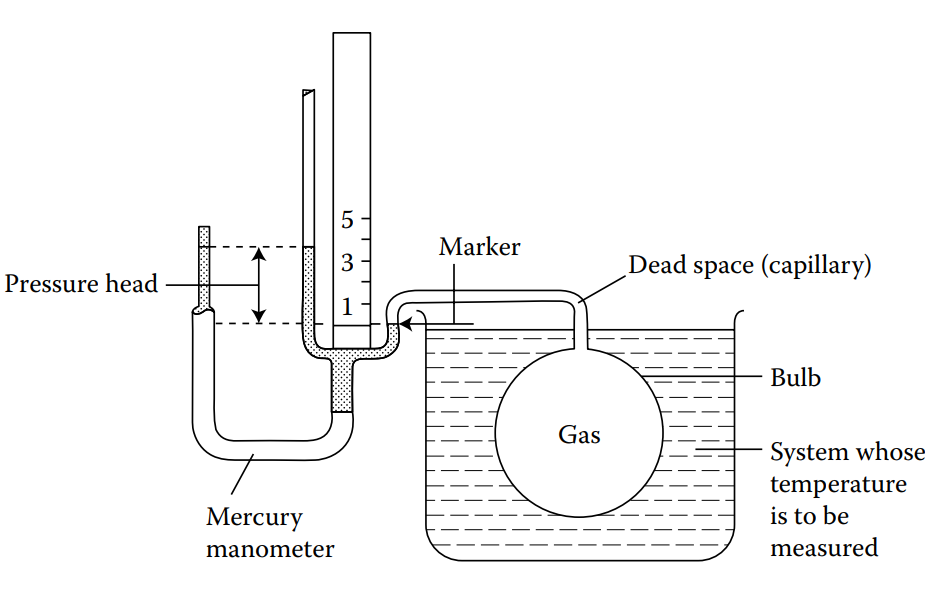
\includegraphics[scale=0.6]{Termometro_gp.png}
\end{figure}

Si considera il prototipo di uno strumento termometrico basato sull'utilizzo di un gas generico, ad esempio ossigeno molecolare $O_2$.\\
La variabile termometrica utilizzata è la pressione del gas.\\
Il dispositivo è composto da:
\begin{itemize}
\item Un bulbo con pareti diatermiche, che andrà posto a contatto con i sistemi su cui si effettua la misura di temperatura. Esso contiene $n$ moli del gas utilizzato.
\item Un tubo contenente mercurio liquido, comunicante con il bulbo, che presenta una scala graduata per la misurazione della pressione di $\mathrm{Hg}$. 
\item Un manometro, ovvero un serbatoio di mercurio regolabile, collegato al tubo, che permette di variare la quantità di mercurio di modo da mantenere costante il volume del gas.
\end{itemize}
Per la misura della pressione è possibile applicare la Legge di Stevino, considerando la differenza di altezza tra la porzione verticale in cui agisce la pressione del gas e quella ad essa parallela, graduata, in cui la pressione è pari a quella atmosferica sommata a quella esercitata dal volume ulteriore di mercurio. Ovvero
\[p = p_{atm} + \rho^{\mathrm{Hg}} g\Delta h \quad con \enspace \, \Delta h = h_1 - h_0\]

\paragraph{Procedura operativa}
\begin{enumerate}
\item Il termometro viene tarato in una cella a punto triplo (tramite immersione) $\rightarrow$ si misura $p_3$ sulla scala graduata.
\item \'E posto a contatto con il corpo di cui si intende misurare la temperatura, agendo con il manometro tra i due passaggi per mantenere il volume del gas nel bulbo costante. Si misura il valore della pressione $p$.
\item Si determina il risultato della misura secondo $\displaystyle \theta(p) = 273.16 \frac{p}{p_3}$
\end{enumerate}
Si osserva che variando il numero di moli si hanno valori differenti di pressione in corrispondenza del punto triplo. Graficando l'andamento per le varie sostanze si osserva che la relazione $\theta\big(p_3(n)\big)$ è lineare con coefficienti angolari differenti. Tuttavia, per $p_3 \rightarrow 0$ tutte le rette convergono a $\theta = 373.15$.
\\Rimuovendo progressivamente il gas dal bulbo, e dunque aumentandone la rarefazione (ovvero la distanza intermolecolare) si va a 'spegnere' il potenziale di LJ (specifico delle varie sostanze), lasciando come unico contributo energetico l'energia cinetica, che si può già evincere corrisponda alla temperatura: dunque \textbf{tutti i gas hanno il medesimo comportamento nel limite} $p 	\rightarrow 0$, ovvero a volume costante $r \rightarrow \infty$.
\infobox{Pendenze negative per $\mathrm{H}$ ed $\mathrm{He}$?}{
Osservando il grafico dell'andamento descritto, si osserva che elio ed idrogeno convergono al medesimo limite di temperatura \textit{ma dal basso}, a differenza degli altri gas. La ragione risiede nel fatto che molecole composte da atomi a ridotto numero atomico (1 e 2 rispettivamente) le interazioni elettrostatiche tra dipoli, che sono all'origine delle forze intermolecolari, sono estremamente deboli. Dunque il corrispondente potenziale di Lennard-Jones mostra una forma molto acuta (piccata), ovvero \textit{tende molto rapidamente a $0$ dal basso} all'aumentare della distanza intermolecolare. Dunque si ha una netta dominanza della componente repulsiva su quella attrattiva: l'allontanamento (per rarefazione del gas) non provoca il passaggio da una condizione attrattiva ad una senza interazioni, come avviene negli altri gas, bensì da una \textit{repulsiva} ad una a interazione nulla.\\Dunque l'energia cinetica (di cui, si vedrà, la temperatura è una misura) aumenterà anziché diminuire.
\begin{figure}[h!]
\centering
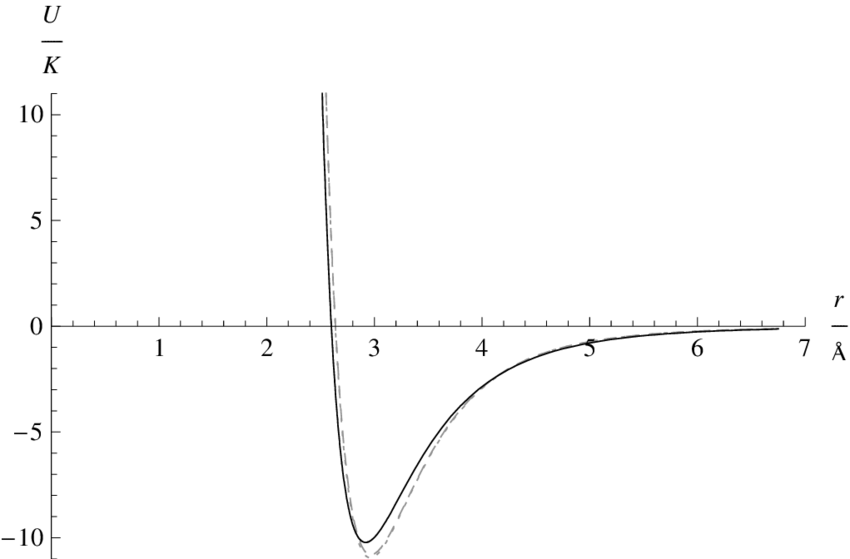
\includegraphics[scale=0.25]{lennardjj.png}
\caption{Potenziale di LJ per l'$\mathrm{He}_2$}
\end{figure}
}

\subsubsection*{Il Gas Perfetto}
\'E quindi possibile definire un modello fisico (approssimazione teorica ma estremamente efficace) denominato \textbf{Gas Perfetto}, che descrive il comportamento di qualunque gas nel limite di elevata rarefazione (unica condizione necessaria!), permettendo la definizione e l'utilizzo della $\theta$ misurata con il termometro a gas. 
\\Il limite fisico di utilizzo di tale strumento è dato dalla più bassa temperatura di liquefazione di un gas, ovvero i $0.5 \, \mathrm{K}$ dell' $\mathrm{{}^3He}$. Per coprire l'intervallo $[0, 0.5[$ sarà necessario svincolare completamente il concetto di temperatura dalla sostanza termometrica.

\subsection{Scala internazionale delle Temperature (ITS)}
\'E definita una scala con una serie di punti fissi misurati con grande precisione tramite termometri a GP. Per misure di valori intermedi essi sono poi utilizzati per tarare altri tipi di termometri (pirometri, ovvero misuratori di radiazione emessa, t. a resistenza di platino, termocoppie platino-rodio o PRT e altri). Essa non sostituisce le scale di riferimento ma ha uno scopo pratico. Definita la prima volta come IPTS (P = Practical) nel 1968, secondo lo standard ITS 90 ha come estremi il punto triplo dell'Idrogeno a $13.8 \, \mathrm{K}$ e il punto di solidificazione del Rame a $1357.77 \, \mathrm{K}$.

\chapter{Sistemi Termodinamici}
Una lunga serie di esperienze ha permesso di determinare le relazioni tra le c.t. dei gas nel limite di GP, fino all'ottenimento dell'\textit{equazione di stato dei gas perfetti}.
\begin{center}
\framebox{
\parbox{\linewidth}{
\vspace{0.3cm}
\textbf{LEGGI DEI GAS PERFETTI}
\begin{description}
\item[I Legge di Gay-Lussac] \hfill a $p$ cost \hspace{2cm} $\displaystyle V = V_0 \beta \theta$ ($V \propto \theta$)
\item[II Legge di Gay-Lussac] \hfill a $V$ cost \hspace{2cm} $\displaystyle p = p_0 \beta \theta$ ($p \propto \theta$)
\begin{center}
con $\beta = 1/273.15 \celsius\mathrm{{}^{-1}}$ 
\end{center}
\item[Legge di Boyle] \hfill a $n, \theta$ cost \hspace{2cm} $\displaystyle V = \frac{cost}{p}$ ($\displaystyle V \propto \frac{1}{p}$)
\item[Legge di Avogadro] \hfill a $p, \theta$ cost \hspace{2cm} $\displaystyle V = cost' \cdot n$ ($V \propto n$)
\item[Equazione di stato dei GP] \hfill $\boxed{\displaystyle pV = nR \theta}$
\end{description}
\vspace{0.3cm}
}
}
\end{center}
Dove i valori con pedice $0$ indicano le c.t. alla temperatura di $0 \celsius$, la temperatura è espressa in $\kelvin{}$ e $R$ è la costante dei gas.
\\Si osserva che consegue dall'equazione che in condizioni normali tutti i gas hanno il medesimo volume molare, corrispondente a $22.4 \, \mathrm{L \, mol^{-1}}$
\\Si ricava inoltre in modo immediato:
\[\alpha = \frac{1}{V} \pdv[•]{•}{\theta} \bigg(\frac{nR \theta}{p}\bigg) = \frac{nR}{pV}= \frac{1}{\theta}\]
\[\frac{1}{k} = - \frac{1}{V} \pdv[•]{•}{p} \bigg(\frac{nR\theta}{p}\bigg) = \frac{nR\theta}{V p^2} = \frac{1}{p}\]

\subsection{Isoterme}
Dall'equazione di stato si ottengono le equazioni delle isoterme nel piano $p-V$, secondo
\[p(V; \theta) = \frac{nR\theta}{V}\]
esse sono dunque delle iperboli. 

\section{Trasformazioni termodinamiche}
\begin{description}
\item[Trasformazione termodinamica] processo in cui variano le proprietà (e dunque le c.t.) di un sistema termodinamico
\end{description}
Tramite trasformazioni cambia lo stato del sistema, ovvero la sua configurazione. Tuttavia, durante la trasformazione è impossibile rappresentare stati intermedi sui grafici: per quanto notato anche in precedenza, non si tratta di stati all'equilibrio, e dunque le c.t. non hanno valori uniformi.
\\Tuttavia è possibile costruire un modello, quello delle \textbf{trasformazioni quasistatiche}.
\begin{description}
\item[Trasformazione quasistatica (q.s.)] una trasf. termodinamica che procede attraverso una successione di infiniti stati all'equilibrio differenti di infinitesimi.
\end{description}
Si hanno quindi curvi corrispondenti a trasformazioni isoterme (le curve già viste), isobare (a pressione costante) e isocore (a volume costante).
\\A livello pratico, tali trasformazioni sarebbero realizzabili secondo le seguenti procedure:
\begin{itemize}
\item \textbf{Isobara} per ogni variazione infinitesima di volume del sistema idrostatico, ottenuta diminuendo il peso posto sul pistone, lo si pone a contatto con un termostato con temperatura maggiore di un infinitesimo del precedente, iterando fino al raggiungimento del volume finale
\item \textbf{Isocora} per ogni variazione infinitesima di temperatura, ottenuta sostituendo il termostato come in precedenza, si incrementa la pressione sul pistone aggiungendo masse infinitesime ulteriori.
\end{itemize}

\section{Gas Reali}
Lontano dal limite di G.P., è necessario apportare delle correzioni all'equazione di stato per tenere conto delle proprietà specifiche dei vari gas. Sono possibili due approcci. 
\subsection{Sviluppo del viriale}
Si definisce il \textbf{fattore di compressione} $\displaystyle z \equiv \frac{pV}{nR\theta}$, che quantifica l'allontanamento dal modello ideale. Quindi si sviluppa in serie in $p$ per $p \rightarrow 0$:
\[z(p) = 1 + Ap + Bp^2 + C p^3 + ...\]
con i coefficienti da determinarsi tramite fit sui dati sperimentali (dipendono dalla temperatura). Alternativamente si sviluppa nel volume molare $\ds \molvol = \frac{V}{n} \propto \frac{1}{\rho}$:
\[z\big(\frac{1}{\molvol}\big) = 1 + \frac{A'}{\molvol} + \frac{B'}{\molvol^2} + ...\]
\subsection{Equazione di Van der Waals}
Alternativamente si adotta un approccio \textit{empirico}, valutando modifiche all'equazione sulla base dello studio dell'andamento del potenziale di L-J. 
\\Per distanze inferiori a $r_{min}$ domina il termine repulsivo $\propto r^{-12}$, fino ad un \textbf{muro di potenziale} per $r \rightarrow 0$: ciò corrisponde all'impenetrabilità (e quindi non compenetrabilità) delle molecole, che non possono essere quindi assunte puntiformi. Esse occupano un volume minimo costante proporzionale al loro numero, e quindi alle moli. Esso è denominato covolume
\[V_{reale} = V_{ideale} + \underbrace{b \cdot n}_{cov.} \]
Si osserva poi che la pressione (come sarà poi visto approfonditamente) è la manifestazione macroscopica degli urti delle molecole sulle pareti che delimitano il sistema idrostatico. La presenza di interazioni intermolecolari attrattive per distanze maggiori a $r_{min}$, ove domina il termine $\propto - r^{-6}$, diminuisce l'impulso scambiato con le pareti, riducendo la quantità di moto delle molecole $^1$; invece un maggior numero di molecole implica un numero maggiore di impatti. Dunque la diminuzione del contributo della singola molecola $\dd[•]{p}$ è proporzionale a $\rho$ per $^1$, mentre la diminuzione complessiva è data da $N \cdot \dd[•]{p}$. Dunque $\displaystyle \dd{p}_{tot} \propto \rho^2$, ovvero $\displaystyle \dd{p}_{tot} \propto \frac{n^2}{V^2} = \frac{1}{\molvol^2}$. Indicando la costante di proporzionalità con $a$ si ha 
\[p_{reale} = p_{ideale} - \underbrace{a \frac{n^2}{V^2}}_{\dd{p}}\]
Sostituendo nell'eq. di stato si ottiene
\begin{center}

\framebox{
\parbox{\linewidth}{
\vspace{0.3cm}
\textbf{EQ. DI STATO DI VAN DER WAALS} \hfill $\displaystyle \bigg(p + a\frac{n^2}{V^2}\bigg) (V - bn) = nR\theta$ \quad \bigg| \quad $\displaystyle \bigg(p + \frac{a}{\molvol^2}\bigg) (\molvol - b) = R \theta$
\vspace{0.3cm}
}
}

\end{center}
ove $a$, $b$ sono dette \textit{costanti di Van der Waals} specifiche di ogni gas. Si osserva che in condizioni standard le correzioni relative sul volume e sulla pressione sono nell'ordine dello $0.1\%$. 
\\Ottenendo l'espressione di $p(V)$ si rappresentano quindi le curve nel piano $p-\molvol$), considerando in particolare le isoterme. 
\[p(V) = \frac{nR\theta}{\molvol - b} - \frac{a}{\molvol^2}\]
\begin{itemize}[label=$\square$]
\item Per $\theta$ elevato il primo termine risulta dominante, dunque per $b$ ridotto la curva tende all'iperbole equilatera dei GP, con asintoto a sinistra a $\molvol = b$ (incomprimibilità!)
\item Per un particolare valore di temperatura, definito $\theta_C$ (critico) si ha un flesso orizzontale. Imponendo l'annullamento della derivata prima e seconda della pressione rispetto al volume si ottiene:
\[\mathrm{v}_C = 3 b \quad \theta_C = \frac{8 a}{27 R b} \quad z_C = \frac{p_C \mathrm{v_C}}{R \theta_C} = \frac{3}{8} = 0.375\]
\begin{proof}
\[\begin{cases} \displaystyle \pdv[•]{p}{\molvol} = 0 \\ \\\displaystyle \pdv[2]{p}{\molvol} = 0
\end{cases} \implies \begin{cases} \displaystyle \frac{2a}{\molvol^3} = \frac{R \theta}{(\molvol - b)^2}\\ \\\displaystyle \frac{2 R \theta}{(\molvol - b)^3} = \frac{6a}{\molvol^4}
\end{cases} \implies \begin{cases} \displaystyle \molvol = 3b \\ \\ \displaystyle 2a(2b)^2 = R \theta (3b)^3
\end{cases} \implies \begin{cases} \displaystyle \theta_C = \frac{2a (4b^2)}{R (27b^3)} = \frac{8a}{27Rb} \\ \\ \displaystyle \molvol_C = 3b
\end{cases} \implies\]
\[\implies p_C = \frac{R \theta_C}{2b} - \frac{a}{9b} = \frac{a}{27b^2} \implies z_C = \frac{p_C \molvol_C}{R \theta_C} = \frac{3}{8} 0.375\]
Che si osserva essere indipendente dalla sostanza (come verificato sperimentalmente).
Viceversa è anche possibile ricavare le costanti di Van der Waals dalla \textbf{curva critica} secondo:
\[a = \frac{9}{8} R \theta_C \molvol_C \quad \quad \quad b = \frac{\molvol_C}{3}\]
\end{proof}
\item Per $\theta < \theta_C$ la curva ha un andamento simil-sinuisoidale con massimi e minimi. Tuttavia per determinati intervalli ciò non corrisponde a quanto osservato sperimentalmente: raggiunto un certo valore $V_G$ del volume (o $\molvol_G$ corrispondente) la diminuzione del volume non comporta alcuna variazione della pressione. Si osserva invece la formazione di condensa: si sta infatti verificando una transizione di fase (verso la f. liquida). Una volta completata la transizione, ovvero raggiunto il $V_L$, la curva diviene pressoché verticale, a causa dell'incomprimibilità dei liquidi.
\end{itemize}
Diminuendo ulteriormente la temperatura, si osserva che i valori di $V_L$ e $V_G$ si allontanano. Effettuando un inviluppo sui segmenti orizzontali per le varie temperature subcritiche, ovvero determinando una curva tangente ai punti estremi, si ottiene una parabola con vertice in $\theta_C$, dove è tangente all'isoterma.
\\Ciò permette di realizzare il \textbf{Diagramma di Fase} della sostanza, in cui varie porzioni del piano rappresentano le varie fasi, delimitate dalle curve di saturazione.
\\Per stati nella zona sottesa dalla parabola determinata, il vapore si trova in uno stato definito \textbf{vapore saturo}. Per ogni valore di $V$ (o $\molvol$) compreso tra gli estremi del segmento, e per una data temperatura (o equivalentemente una data pressione) il VS raggiunge l'equilibrio quando il processo di liquefazione di molecole del vapore (a causa degli urti anelastici con la superficie) e quello di evaporazione ('liberazione' per agitazione termica delle molecole superficiali) sono bilanciati. In tal caso il numero di moli di molecole nelle due fasi ($n_L$, $n_G$) resta costante, con il rapporto $\displaystyle \frac{n_L}{n_G} = \frac{\molvol_G - \molvol}{\molvol - \molvol_L}$ con $\molvol_i = V_i \big/ n_i$.
\begin{proof}
\[V_L + V_G = n_L \molvol_L + n_G \molvol_G = n \molvol \quad \frac{n_L}{n_G} = \frac{V_L \big/ \molvol_L}{V_G \big/ \molvol_G}\]
Imponendo $n_L + n_G = n$ (sistema chiuso) si ha
\[n_G \molvol_G + n_L \molvol_G = (n_L + n_G) \molvol \implies n_G(\molvol_G - \molvol) = n_L (\molvol - \molvol_L)\]
\end{proof}
Diminuendo il volume resta costante il numero di molecole che passano da una fase all'altra (pelo del liquido resta il medesimo) in quanto dipende esclusivamente dall'agitazione termica, ovvero dalla temperatura. Tuttavia anche la densità si mantiene costante, a spese di $n_G$.
\\~\\Per temperature supercritiche l'energia cinetica delle molecole è troppo elevata perché possa avvenire l'aggregazione e dunque la transizione di fase. Si osserva inoltre che per sistemi aperti l'evaporazione (non l'ebollizione!) si verifica a qualsiasi temperatura, lungo un tempo determinato dalla probabilità di rottura dei legami ad idrogeno, ovvero alla distribuzione delle energie cinetiche (vd Teoria Cinetica).
\subsubsection*{Costruzione di Maxwell}
\'E possibile determinare i valori di $V_L$ e $V_G$ dalla curva prevista dal modello di Van der Waals per temperature subcritiche, tramite un procedimento analitico. 
\\Il metodo della costruzione di Maxwell prevede di tagliare orizzontalmente la curva, di modo da ottenere due aree sottese (una sopra e una sotto la retta orizzontali) uguali. I volumi estremi intercettati sono quelli cercati.
\\Si osserva che per volumi compresi tra $V_L$ e il minimo locale e tra il massimo locale e $V_G$ la derivata della curva è negativa, ovvero si tratta di stati di equilibrio stabile e quindi realizzabili sperimentalmente; per la porzione intermedia invece la derivata positiva implica si tratti di equilibri instabili, e quindi irrealizzabili.

\subsection{Diagrammi di fase di sostanze pure}
Si tratta di diagrammi tridimensionali nello spazio $\theta, V, p$, in cui le curve di saturazione e transizione generano una superficie denominata \textbf{superficie pVT} ($pV\theta$).
\\Le proiezioni della stessa sul piano (p,V) e (p,$\theta$) danno poi i diagrammi di fase bidimensionali.
\subsubsection{Piano (p,T)}
Sono rappresentate le curve di transizione, descritte dalle equazioni di Clausius-Clapeyron (vd più avanti). Per Temperature e pressioni supercritiche, si ha lo stato di \textbf{fluido supercritico}, che presenta proprietà macroscopiche miste di liquidi (densità) e aeriformi (viscosità). Esso è presente, ad esempio, nei vulcani sottomarini (approssimando un andamento con la profondità $\displaystyle p(h) = \frac{h}{10 \mathrm{m}} \, \mathrm{atm}$ si ha $p(2 \mathrm{km}) = 200 \, \mathrm{atm}$!)
\\Si osserva inoltre che la temperatura di ebollizione varia con la pressione (o viceversa) e che è possibile transire di da liquido ad aeriforme diminuendo la pressione a temperatura costante: si ha il processo di \textbf{cavitazione}.
\paragraph{Si applichi Gibbs} per sistema monocomponente:
\begin{itemize}
\item Nelle regioni piene $F = 1$, dunque $N = 2$: il sistema può trovarsi in qualsiasi punto della regione, in quanto le due c.t. sono indipendenti
\item Lungo le curve $F =2$, dunque $N = 1$: gli stati possibili giacciono sulla specifica curva $p(\theta)$
\item Nel punto triplo $F = 3$, dunque $N = 0$: si realizza solo in condizioni specifiche, da cui la variazione di una qualsiasi c.t. intensiva farebbe allontanare il sistema.
\end{itemize}
Si osservi che è possibile applicare la Regola solo per quanto riguarda la proiezione $(p, \theta)$ in quanto si tratta di variabili intensive.

\chapter{Teoria cinetica dei gas}
\section{Interpretazione microscopica: uno schema}
Il seguente schema concettuale generale descrive il processo scientifico:

\begin{center}
* schema *
\end{center}

La teoria di base della TCG è la meccanica newtoniana. Il modello sviluppato è invece il:
\section{Modello cinetico}
Esso è costituito da $N$ molecole moventi di moto rettilineo uniforme all'interno di una scatola cubica, di cui occupano tutto il volume. Le assunzioni di base del modello sono:
\begin{enumerate}
\item $N$ è sufficientemente grande
\item Il covolume è trascurabile, ovvero le molecole possono essere considerate puntiformi
\item Le interazioni a lungo range sono trascurabili (no L-J) e quelle a corto raggio (urti tra molecole e con le pareti) sono completamente elastiche
\item Si ha il \textbf{caos molecolare}, ovvero  \textbf{omogeneità} (la densità è considerabile uniforme) e \textbf{isotropia} (non vi sono direzioni privilegiate per il moto delle particelle, ovvero il gas è macroscopicamente fermo)
\end{enumerate}
Gli assunti 2. e 3. implicano ci si stia ponendo nel campo di applicabilità del modello di Gas Perfetto.

\paragraph{Aria in condizioni standard soddisfa requisiti?} 
\begin{itemize}
\item Si considera un volumetto $V = 1 \, \mathrm{cm^3}$. Si ha $\displaystyle N = \frac{pV}{R \theta} N_A \approx 10^{19}$ molecole, un numero sufficientemente grande per consentire l'approccio statistico (anche su scala locale!)
\item Il $99 \% $ delle molecole è rappresentato da $N_2$ e $O_2$, che presentano una forma a 'fagiolo' con lunghezza maggiore $d = 1.7 \angstrom$. Approssimando a sfere di raggio $d/2$ si ottiene un covolume $\displaystyle = N \frac{4}{3}\pi \bigg(\displaystyle \frac{d}{2}\bigg)^3 \approx 6 \times 10^{-11} \meters{}{3}$ e dunque un rapporto $\displaystyle r \equiv \frac{V_{mol}}{V} \approx 6 \times 10^{-5}$
\item Approssimando la disposizione omogenea con una griglia (un reticolo) con molecole nei vertici si determina il passo:
\[N = \frac{V}{\lambda^3} \implies \lambda = \bigg(\frac{V}{N}\bigg)^{\frac{1}{3}} \approx 34 \angstrom \implies r \equiv \frac{\lambda}{d} \approx 20\]
Poiché $d \sim r_{min}$, a distanze tanto superiori le interazioni sono trascurabili
\item L'omogeneità è già stata assunta nel punto precedente. Se tutte le molecole hanno approssimativamente uguale massa, la condizione di isotropia $\vec{P} = 0$ si traduce in $\displaystyle \sum_i \vec{v}_i = 0$, ovvero per ogni molecola che si muove in una direzione ve ne è una che si muove sulla medesima ma in verso opposto. 
\end{itemize}

\subsection{Pressione}
Si considerano gli urti elastici su una delle pareti della scatola (l'assunzione di isotropia permette di sceglierne una qualsiasi). Sia essa quella di destra, orientata perpendicolarmente all'asse $x$ e indicata in figura con $S_x$.
\\Per un urto elastico con $M_{parete} \gg m_{mol}$ si ha:
\[\begin{cases} \displaystyle v_{ix}' = - v_{ix} \\ \\ \displaystyle v_{iy}' = v_{iy} \implies \Delta q_{iy} = 0\\ \\ \displaystyle v_{iz}' = v_{iz} \implies \Delta q_{iz} = 0
\end{cases} \implies \Delta q_{ix} = \Delta q_i = - 2m v_{ix}\]
In un dato $\Delta t$, il numero di urti sulla parete della $i$-esima particella dipende dal solo moto su $x$ (in quanto il modulo delle altre componenti rimane invariato e i tre moti sono indipendenti). La variazione totale della quantità di moto su $x$ è quindi calcolata moltiplicando la variazione per ogni particella per il numero di urti corrispondenti e sommando sulle particelle
\[n°_{urti}(i) = \frac{|v_{ix}| \Delta t}{2L} \implies |\Delta Q_x| = \sum\limits_{i=1}^N |\Delta q_{ix}| \cdot n°_{urti}(i) = \sum\limits_{i=1}^N \frac{2 m |v_{ix}| \cdot |v_{ix}| \Delta t}{2L} = \frac{m \Delta t}{L} \sum\limits_{i=1}^N v_{ix}^2\]
assunta la massa uniforme. La forza media è data dalla variazione di quantità di moto complessiva, ovvero l'impulso esercitato, sull'intervallo di tempo. La pressione si ottiene quindi dividendo tale forza per la superficie su cui è applicata:
\[|F_x| = \frac{|\Delta Q_x|}{\Delta t} = \frac{m}{L} \sum\limits_{i=1}^N v_{ix}^2 \implies p_x = \frac{|F_x|}{S_x} = \frac{m}{S_x \cdot L} \sum\limits_{i=1}^N v_{ix}^2 = \frac{m}{V} \sum\limits_{i=1}^N v_{ix}^2\]
Si ricava analogamente l'espressione per pareti ortogonali alle altre due direzioni, ovvero $S_y$ e $S_z$. Per $N$ grande si applica la condizione di isotropia, ovvero si assume che i valori di $v_{ij}$ siano equamente distribuiti sulle tre direzioni $j = x, y, z$. Ciò implica
\[p_x = p_y = p_z \equiv p\]
ovvero si ha pressione idrostatica: si è di fatto ricavato il \textbf{Principio di Pascal}, secondo cui la pressione è una grandezza scalare indipendente dall'orientamento della superficie su cui è applicata. Dunque
\[p = \frac{1}{3}(p_x + p_y + p_z) = \frac{m}{3V} \sum\limits_{i=1}^N [v_{ix}^2 + v_{iy}^2 + v_{iz}^2] = \frac{m}{3V} \sum\limits_{i=1}^N v_{i}^2 \implies
pV = \frac{m}{3}\sum\limits_{i=1}^N v_{i}^2\]
Si introduce quindi la \textbf{velocità quadratica media} $\langle v^2 \rangle$, definita come valore di aspettazione del quadrato del modulo delle velocità molecolari,  e successivamente l'\textbf{energia cinetica molecolare media} $\langle \varepsilon \rangle$:
\[\langle v^2 \rangle \equiv \mathbb{E}[v^2] = \frac{\sum_i v_i^2}{N}\implies pV = \frac{m}{3} N \langle v^2 \rangle = \frac{2}{3} N \bigg(\frac{1}{2}m \langle v^2 \rangle\bigg) = \frac{2}{3}N \big\langle \frac{1}{2}mv^2 \big\rangle = \frac{2}{3}N \langle \varepsilon \rangle\]
in quanto la massa è assunta uniforme. Invocando l'equazione di stato dei gas perfetti:
\[nR\theta = \frac{2}{3}N \langle \varepsilon \rangle \implies \varepsilon = \frac{3}{2}\frac{n}{N} R \theta = \frac{3}{2} \frac{R}{N_a}\theta = \frac{3}{2} k_B \theta\]
Si è così stabilito un \textit{ponte macro-micro} tramite l'introduzione di quantità medie che permettono di considerare una caratterizzazione globale del sistema prescindendo dalla conoscenza esatta del microstato.
\\La temperatura è così caratterizzata come grandezza \textbf{emergente} proporzionale al valor medio delle energie cinetiche molecolari, dunque ad esse collegata per via statistica. Tali d.o.f. interni del sistema, \textit{variabili nascoste} microscopiche, producono una quantità misurabile macroscopicamente.
\\~\\Si ha quindi la giustificazione del comportamento dei gas nel limite del GP: se per il potenziale $U \rightarrow 0$, si ha $E \rightarrow \varepsilon$ con $\langle \varepsilon \rangle \propto \theta$.
\paragraph{Osservazioni}
\begin{itemize}
\item La costante di Boltzmann è misurabile sperimentalmente, ad esempio attraverso l'esperimento di Perrin sul moto browniano
\item Dal 2019 $k_B$ è stata assunta come costante fondamentale senza incertezza per la ridefinizione del$\kelvin{}$ da parte del BIPM. In tal modo la precisione della scala non è più vincolata a quella della riproduzione delle specifiche condizioni di $S_3$, è può anzi in futuro divenire arbitrariamente elevata con la possibilità di ridefinizione dei punti fissi.
\end{itemize}
La costante di Boltzmann rappresenta un vero e proprio fattore di conversione tramite cui la temperatura è ridefinita come una grandezza energetica.
\\Difatti la ridefinizione della scala Kelvin è la seguente:
\begin{quote}
$1 \kelvin{}$ corrisponde alla temperatura di una sostanza che ha $\displaystyle \frac{k_B}{2} \joule{}$ di energia cinetica media per grado di libertà cinetico.
\end{quote}
Per il numero di d.o.f. si fa ricorso al \textbf{Teorema di equipartizione dell'energia} (vd più avanti)
\begin{center}

\framebox{
\parbox{\linewidth}{
\vspace{0.3cm}
\textbf{TEOREMA DI EQUIPARTIZIONE DELL'ENERGIA} A ogni d.o.f. che si presenta in forma di termine quadratico (quadraticamente) nel calcolo dell'energia cinetica corrisponde un termine $\displaystyle \frac{1}{2}k_B \theta$ \vspace{0.3cm}
}
}
\end{center}
Dunque
\[\langle \varepsilon \rangle = \frac{\nu}{2} k_B \theta \implies \theta = \frac{2 \langle \varepsilon \rangle}{k_B \cdot \nu}\]
\textbf{RELATIVIT\'A SPECIALE }\hrulefill
\\Il limite superiore alla velocità determinato dalla SR implica un limite ad $\varepsilon$ e dunque a $\theta$? No, in quanto l'espressione classica per l'energia cinetica non vale fuori dal limite classico! Per velocità prossime a $c$, la differenza di energia necessaria ad imprimere un'ulteriore accelerazione diverge; dunque $\theta \rightarrow \infty$.
\\\hrule

\subsubsection{Legge di Dalton}
Siano dati due (o più) GP occupano insieme un dato volume, e noti il rispettivi numeri di moli e le \textit{pressioni parziali}, ovvero le pressioni esercitate da ognuno occupando interamente il volume in assenza degli altri. Si ha: $\displaystyle p_i = \frac{n_i R \theta_i}{V}$ e  $n = \sum n_i$. Si osserva che $\langle \varepsilon_i \rangle = \frac{3}{2} k \theta_i$ e che per la media complessiva si ha: \[\langle \varepsilon \rangle = \frac{\sum n_i \langle \varepsilon_i \rangle}{\sum n_i} \implies \theta = \frac{2\langle \varepsilon \rangle}{3k} = \frac{2 \sum n_i \langle \varepsilon_i \rangle}{3 k \sum n_i} \implies pV = \big(\sum n_i\big) R \frac{2 \sum n_i \langle \varepsilon_i \rangle}{3 k \big(\sum n_i\big)} = R \sum \frac{2}{3k} n_i \langle \varepsilon_i \rangle =\]
\[= R \sum n_i \theta_i = \sum R n_i \theta_i = \sum p_i V \implies p = \sum p_i\]

\section{Distribuzione delle velocità molecolari (di Maxwell)}
Si intende determinare la PDF della variabile continua $v$, corrispondente al modulo della velocità molecolare
\[\rho \, : \, [0, +\infty [ \, \rightarrow \, [0,1[ \enspace t.c. \enspace P(v < v' < v + \dd{v}) = \rho(v)\dd{v}\]
\\Si assume che il sistema in esame sia all'equilibrio termodinamico, e dunque quello termico ($\theta$ è uniforme e costante) e isolato. Qualsiasi sistema che soddisfi tali assunti tenderà a presentare una configurazione di velocità molecolari descritta dalla Maxwelliana; anche partendo da una distribuzione differente in un certo lasso di tempo urti anelastici condurranno alla distribuzione qui derivata.
\\Per ottenere $\rho$ è in primo luogo necessario determinare le distribuzioni delle singole componenti, $f(v_x)$, $f(v_y)$, $f(v_z)$. Si determina quindi la \textbf{PDF congiunta} definita secondo
\[P(v_x < v_x' < v_x + \dd{v_x}, v_y < v_y' < v_y + \dd{v_y}, v_z < v_z' < v_z + \dd{v_z}) = F(v_x, v_y, v_z) \dd{v_x} \dd{v_y} \dd{v_z}\]
ovvero la funzione che quantifica la probabilità che la terna di velocità di una molecola qualsiasi si trovi nel cubetto infinitesimo dello spazio delle velocità.
\\Nell'ipotesi del caos molecolare, le distribuzioni delle tre componenti sono indipendenti, ovvero l'informazione su ciascuna non influisce su quella delle altre. Segue che $F$ sia data secondo:
\[F(v_x, v_y, v_z) = f(v_x) f(v_y) f(v_z) \enspace ^1\]
Inoltre per l'isotropia (che costituisce un \textbf{fatto fisico}) $F$ non può presentare una dipendenza dal verso e/o dalla direzione di $v$: deve essere funzione del solo modulo, ovvero della distanza del punto $(v_x, v_y, v_z)$ dall'origine dello spazio delle velocità$^2$.
\\Da $^1$ e $^2$ si ottiene:
\[F(v_x^2 + v_y^2 + v_z^2) = f(v_x) f(v_y) f(v_z)\]
L'unica funzione in grado di soddisfare entrambe le formulazioni di $F$ è l'\textbf{esponenziale}. \\Infatti $e^{\sum a_i} = \prod e^{a_i}$. Si assume quindi un'\textbf{ipotesi di lavoro} sulla forma di $f$:
\[f(v_i) = \eta e^{\pm \xi v_i^2} \implies
 F(v_x, v_y, v_z) = \eta^3 e^{\pm \xi (v_x^2 + v_y^2 + v_z^2)} = \eta^3 e^{\pm \xi v^2}\]
\'E quindi necessario determinare i due parametri ed il segno dell'esponente (assunto $xi > 0$). Poiché il sistema ha un'energia finita, quest'ultimo dev'essere negativo, di modo da avere probabilità tendenti a $0$ per moduli delle velocità tendenti a $\infty$: $\displaystyle F \xrightarrow[v \rightarrow +\infty]{} 0$
\\Si impone quindi la normalizzazione, considerando il valore noto per l'integrale errore:
\[\int_{-\infty}^{+\infty}f(v_i)\mathrm{d}v_i = \eta \int_{-\infty}^{+\infty}e^{-\xi v_i^2}\mathrm{d}v_i = \eta \frac{1}{\sqrt{\xi}} \int_{-\infty}^{+\infty} e^{-\xi v_i^2}\sqrt{\xi}\mathrm{d}v_i \implies
t = \sqrt{\xi}v_i \implies \eta \frac{1}{\sqrt{\xi}} \int_{-\infty}^{+\infty}e^{-t^2}\mathrm{d}t =\]
\[= \eta \frac{\sqrt{\pi}}{\sqrt{\xi}} = 1 \implies \eta = \sqrt{\frac{\xi}{\pi}}\]
Si impone ora la relazione determinata in precedenza per l'energia cinetica media e dunque la velocità quadratica media, sotto l'assunzione di massa molecolare uniforme:
\[\langle \varepsilon \rangle = \frac{3}{2} k \theta \implies \langle v^2 \rangle = \frac{3 k \theta}{m}\]
\infobox{VALORE DI ASPETTAZIONE}{Data una variabile continua $x$ distribuita secondo la PDF $\phi(x)$ su tutta la retta il \textbf{valore di aspettazione} di una qualsiasi funzione $a(x)$ è dato da
\[\mathbb{E}[a(x)] = \langle a \rangle = \int_{-\infty}^{+\infty} a(x) \phi(x) \, \mathrm{d}x\]
(intuitivamente corrisponde ad una 'media pesata' dei valori di $a$). Se $x$ assume valori su un qualsiasi intervallo, si sostituiscano nell'espressione precedente gli estremi dello stesso come estremi di integrazione.}
\[\langle v_i^2 \rangle = \int_{-\infty}^{+\infty} v_i^2 f(v_i)\, \mathrm{d}v_i = \eta \int_{-\infty}^{+\infty} v_i^2 e^{-\xi v_i^2}\, \mathrm{d}v_i\]
Integrando per parti:
\[\eta \int_{-\infty}^{+\infty} v_i \cdot v_i e^{- \xi v_i^2}\, \mathrm{d}v_i = - \eta \frac{1}{2 \xi} v_i e^{- \xi v_i^2}\bigg|_{-\infty}^{+\infty} + \frac{\eta}{2\xi} \int_{-\infty}^{+\infty} e^{-\xi v_i^2}\, \mathrm{d}v_i\]
Ora,
\[\limit{v_i}{+\infty} e^{- \xi v_i^2} v_i = \frac{v_i}{e^{\xi v_i^2}} = 0 \quad \limit{v_i}{-\infty} \frac{v_i}{e^{\xi v_i^2}} = 0\]
in quanto la divergenza esponenziale è di ordine superiore a quella lineare. Il secondo termine ottenuto procedendo per parti si integra come in precedenza:
\[\mean{v_i^2} = \eta \sqrt{\frac{\pi}{\xi}} \big(\frac{1}{2 \xi}\big) = \frac{1}{2 \xi}\]
in quanto i primi due fattori sono uno il reciproco dell'altro.
\\Distribuendo ora la somma nel calcolo del valore di aspettazione, considerata l'indipendenza delle tre componenti:
\[\mean{v^2} = \mean{v_x^2 + v_y^2 + v_z^2} = \mean{v_x^2} + \mean{v_y^2} + \mean{v_z^2} = \frac{3}{2 \xi} \implies \frac{3}{2 \xi} = \frac{3k \theta}{m} \implies \xi = \frac{m}{2 k \theta} 	\implies \eta = \sqrt{\frac{m}{2 \pi k \theta}}\]
Da cui
\[f(v_i; \theta, m) = \sqrt{\frac{m}{2 k \theta}} e^{\displaystyle - \frac{m v_i^2}{2 k \theta}}\]
si tratta di una distribuzione normale centrata in $0$ (come ragionevole attendersi sotto l'assunzione di isotropia) con varianza $\ds \sigma_i^2 = \frac{k \theta}{m}$ e SD $\ds \sigma_i = \sqrt{\frac{k \theta}{m}}$.
\\Dunque un aumento della temperatura comporta l'abbassamento del picco (diminuzione della probabilità di trovare molecole 'ferme') e il popolamento delle code (aumento probabilità di trovare molecole con velocità, ovvero energie cinetiche, elevate). $F$ diviene
\[F(v; \theta, m) = \bigg(\frac{m}{2 \pi k \theta}\bigg)^{\frac{3}{2}} e^{\displaystyle - \frac{mv^2}{2 k \theta}}\]
Per ottenere quindi la $\rho (v)$ è necessario integrare, per ogni valore del modulo $v$, sul guscio sferico nello spazio delle velocità di raggio $v$ e spessore infinitesimo $\dd{v}$. Per isotropia, infatti, la probabilità di ognuno dei punti del guscio è uguale.
\[V_{sfera} = \frac{4}{3} \pi v^3 \implies \dd{V} = 4 \pi v^2 \dd{v} = V_{guscio} \implies \rho(v) \dd{v} = F(v_x, v_y, v_z) 4 \pi v^2 \dd{v}\]
da cui la \textbf{distribuzione di Maxwell} (o delle velocità molecolari)
\[\boxed{\rho (v; \theta) = \frac{4}{\sqrt{\pi}} \bigg(\displaystyle \frac{m}{2k \theta}\bigg)^{ \frac{3}{2}} v^2 e^{\displaystyle - \frac{mv^2}{2k \theta}}}\]
si nota la presenza del termine di risonanza $v^2$, che causa l'asimmetria della distribuzione. Si osserva inoltre che $\ds \rho \tendsto{v}{0} 0$, in quanto la velocità ha modulo nullo se e solo se si annullano tutte e tre le componenti, ovvero il guscio sferico considerato si riduce ad un punto.
\begin{itemize}
\item Per $\theta$ crescente il picco si sposta verso destra (aumenta l'energia media) e la curva tende alla simmetria
\item Viceversa per $\theta$ decrescente il picco si sposta verso sinistra; al limite la funzione tende alla \textbf{delta di Dirac}, che ha un picco divergente in 0 ed è nulla su tutto il resto della retta, risultando tuttavia normalizzata.
\end{itemize}
Si calcolano dunque alcuni valori rilevanti che descrivono la posizione del 'centro' della distribuzione.
\begin{enumerate}
\item \textbf{La moda} $v_p$, corrispondente al punto di massimo della distribuzione, si ottiene imponendo l'annullamento della derivata prima 
\[\dv[•]{\rho}{v} = \frac{4}{\sqrt{\pi}} \bigg(\displaystyle \frac{m}{2k \theta}\bigg)^{ \frac{3}{2}}e^{\displaystyle - \frac{mv^2}{2k \theta}} \bigg(2v - \frac{2 m v^3}{2 k \theta}\bigg) \bigg|_{v_p}^{•} = 0\]
Assunto $v_p \neq 0$ in quanto in $0$ si ha un minimo locale, si ha
\[\frac{mv_p^2}{k \theta} = 2 \implies v_p = \sqrt{\frac{2 k \theta}{m}} = \sqrt{\frac{2 R \theta}{\mathcal{M}}}\]
ove $\mathcal{M}$ è la massa molare.
\item \textbf{Velocità quadratica media} il calcolo verifica semplicemente la condizione imposta per la determinazione dei parametri: 
\[\mean{v^2} = \frac{3 k \theta}{m} = \frac{3 R \theta}{\mathcal{M}}\]
\item \textbf{Velocità media}
\[\mean{v} = \int_{0}^{+\infty} v^3 \frac{4}{\sqrt{\pi}} \bigg(\displaystyle \frac{m}{2k \theta}\bigg)^{ \frac{3}{2}} e^{\displaystyle - \frac{mv^2}{2k \theta}}\, \mathrm{d}v = \frac{4}{\sqrt{\pi}} \integral{0}{+\infty}{\bigg( \ds \frac{m}{2k \theta}\bigg)^{\frac{1}{2}}e^{\displaystyle - \frac{mv^2}{2k \theta}} \frac{mv}{2k \theta}}{v}\]
Si pone $\ds x = - \frac{mv^2}{2k\theta}$, da cui $\dd{x} = - \frac{mv}{k\theta}\dd{v}$ e $\ds v = \sqrt{- \frac{2k\theta}{m} x}$.
\[\mean{v} = \frac{4}{\sqrt{\pi}} \bigg(\displaystyle \frac{m}{2k \theta}\bigg)^{ \frac{1}{2}} \integral{0}{-\infty}{\bigg(- \frac{2k\theta x}{m}\bigg) e^x \bigg(- \frac{1}{2}\bigg)}{x} = \frac{2\sqrt{2}}{\sqrt{\pi}} \bigg(\frac{k \theta}{m}\bigg)^{\frac{1}{2}} \int_{0}^{-\infty} x e^x \, \mathrm{d}x = \frac{2\sqrt{2}}{\sqrt{\pi}} \bigg(\frac{k \theta}{m}\bigg)^{\frac{1}{2}} \bigg[x e^x - e^x \bigg]_0^{+\infty} = \]
\[= \sqrt{\frac{8 k \theta}{\pi m}} \big(0 - (-1) \big) = \sqrt{\frac{8 k \theta}{\pi m}}\]
\end{enumerate}
Si osserva che $\pi > 3$, dunque $\ds \frac{8}{\pi} < \frac{9}{\pi} < \frac{9}{3} = 3$, il che implica $\ds \mean{v} < \sqrt[•]{\mean{v^2}}$.


\subsubsection{Il selettore di velocità}
Si tratta di uno strumento utilizzabile per ottenere sperimentalmente la distribuzione delle velocità molecolari di un gas e poterne dunque verificare la compatibilità con quanto previsto dal modello di Maxwell.\\
Il gas è inizialmente posto in un recipiente e si trova in condizioni di equilibrio, dunque a $\theta$ definita e costante. Viene praticato un foro nella parete, da cui fuoriescono le molecole, e posizionata ad una distanza sufficiente una parete con un'apertura di dimensioni ridotte in corrispondenza della direzione perpendicolare. Essa è denominata \textit{selettore}, e permette appunto di selezionare le sole molecole la cui velocità di uscita secondo la direzione della velocità.\\
Dopo il selettore è quindi posto un cilindro rotante con velocità angolare costante $\omega$, che presenta un foro allineato ai precedenti ed è foderato di una pellicola impressionabile, sensibile all'incidenza delle molecole.\\
La posizione del punto d'impatto di una molecola è legata alla sua velocità, in quanto La distanza tra il punto collocato sulla direzione perpendicolare sulla parete opposta al momento dell'ingresso della molecola nel cilindro e quello impressionato è data dal raggio per l'angolo di rotazione, ovvero dalla velocità angolare del cilindro per il tempo impiegato dalla molecola ad attraversarlo:
\[v = \frac{2 R}{\Delta \tau} \implies \Delta l = \alpha R = \omega \Delta \tau R = \frac{2 \omega R^2}{v}\]
Aprendo la pellicola al termine dell'esperienza, si osservano delle bande corrispondenti ai punti impressionati: tramite un fit si determina la distribuzione di probabilita di $\Delta l$ e quindi, nota l'espressione di sopra per $\Delta l(v)$ si ricava $\rho(v)$, da confrontarsi con la Maxwelliana.\\
Si osserva ovviamente che l'esperimento poggia sull'assunto, comune anche al modello, di isotropia: dunque la distribuzione di velocità in una direzione può essere considerata rappresentativa di quella generale.

\subsection{Ebollizione ed evaporazione}
Come si evince dalla forma della Maxwelliana, indipendentemente dalla temperatura del sistema vi è un numero non nullo di molecole con energie sufficientemente elevata da rompere i legami intermolecolari che realizzano gli stati condensati, e dunque passare alla fase di vapore (aeriforme). In modo formalmente più corretto, tali considerazioni andrebbero effettuate sulla distribuzione dei livelli energetici, ovvero la d. di Boltzmann $\rho (\varepsilon)$.
\\Definita l'energia limite $\varepsilon_{leg}$, si determina la corrispondente $v_{leg}$. Il numero di molecole con energia sufficiente è dato da
\[N_{evap} = \integral{v_{leg}}{+\infty}{\rho(v)}{v}\]
\\L'aumento di $\theta$ comporta solo un maggiore popolamento di tale porzione della distribuzione, il che accelera il processo.
\\Se il liquido si trova a contatto con un termostato, una volta perse le molecole evaporate gradualmente tende a ritornare all'equilibrio termico: dunque nuove molecole vanno a ripopolare la coda e quindi ad evaporare.
\infobox{Per l'acqua}{L'energia del legame ad H è $\ds \approx 0.2 \evolt$, mentre l'energia cinetica media in condizioni standard è $0.04 \evolt$: può esistere acqua liquida (gran parte della Maxwelliana è sotto la velocità limite, e di conseguenza il processo di evaporazione è estremamente lento)}

\subsubsection{Atmosfere planetarie}
Poiché l'aria è composta al $99 \%$ da $N_2$ e $O_2$ si approssima $\mathcal{M} = 32 \grams{} \mols{-1}$. Ponendo l'energia meccanica, somma della cinetica e della potenziale gravitazionale, uguale a $0$ si ha:
\[\frac{1}{2} m v^2 - \frac{GM m}{r} = 0 \implies v^2 = \sqrt{\frac{2G M}{r}}\]
Approssimando il pianeta con una sfera di densità media $\rho$:
\[v^2 = \frac{8 \pi G \rho r^3}{3 r} = \frac{8}{3} \pi G r^2\]
sostituendo a $v^2$ la velocità quadratica media e prendendo la radice:
\[\sqrt{\mean{v^2}} = \sqrt{\frac{3 R \theta}{\molms}} = r \sqrt{\frac{8}{3} \pi G} \implies r = \sqrt{\frac{9 R \theta}{8 G \pi \molms \rho}}\]
La formula trovata giustifica l'assenza di atmosfera, ad esempio, della Luna. Si osserva inoltre che il pianeta è assimilabile ad un termostato; dunque secondo quanto detto prima dopo la perdita di molecole la coda della Maxwelliana è ripopolata nel ritorno all'equilibrio termico, in un processo continuo.

\subsubsection{Ebollizione}
Il fenomeno dell'ebollizione si basa di principio sull'evaporazione, ma a differenza di questa coinvolge l'intero volume di liquido e non solo la superficie; sono dunque necessarie particolari condizioni perché si verifichi.
\\Si abbia ad esempio una pentola. Se le sue pareti presentano delle minime asperità, hanno luogo dei microvortici convettivi che portano alla formazione di centri di enucleazione, ovvero microbolle in cui temporaneamente alcune molecole allo stato di vapore si trovano separate da quelle allo stato liquido (tramite evaporazione).
\\Il destino delle microbolle, che possono andare incontro a implosione o eventuale crescita, è determinato dalle pressioni agenti sulle stesse. La pressione esercitata dal vapore all'interno della bolla è quella di vapore saturo, $p_{vap}$, mentre la pressione esterna è quella idrostatica, che secondo Stevino vale $\ds p_e = p_{atm} + \rho g h$.\\
Per $h$ ridotto il secondo termine è trascurabile (si nota che per $h = 10cm$ si ha $\Delta p \approx 10^4 \pascal{}$, ovvero un o.d.g. inferiore alla pressione atmosferica!).\\La condizione di espansione è dunque 
\[p_{vap} \geq p_{atm}\]
Se la bolla cresce, per Archimede sale fino a giungere alla superficie e liberare le molecole nell'aria.
\\Intercettando la curva di Clapeyron sul piano $(p,\theta)$ si ottiene $\theta_{min} = 100 \celsius$, che è effettivamente la temperatura cui bolle l'acqua a pressione atmosferica.




\subsection{Il libero cammino medio}
\begin{description}
\item[Mean free path] distanza media percorsa da una molecola prima di urtarne un'altra
\end{description}
Si tratta di una grandezza che caratterizza gli urti tra costituenti elementari.\\
Le molecole sono approssimate a corpi sferici di diametro $d$ con velocità media $\overline{v}$.\\
Per determinare il numero di urti in un dato intervallo di tempo $\dd[•]{t}$, si considera un cilindro di raggio $d$ e dunque diametro $2d$, e lunghezza pari allo spazio percorso dalla molecola nell'intervallo di tempo, ovvero $l = \overline{v} \dd[•]{t}$. La molecola andrà ad urtare tutte quelle il cui centro giace all'interno del cilindro descritto (come si evince in modo intuitivo). Assunta una densità uniforme, si ottiene $\ds N_{cil} = \frac{N}{V} V_{cil}$.\\
Si considera quindi la sezione d'urto delle molecole (cross section), in questo caso corrispondente alla sezione trasversa del cilindro, il cui raggio è dato dalla distanza tra i centri delle molecole al momento dell'impatto, ovvero a $d$:
\[\sigma = \pi d^2\]
Si determina la frequenza di collisione
\[f = \frac{n°_{urti}}{\dd{t}} = \frac{V_{cil} \frac{N}{V}}{\dd[•]{t}} = \frac{\sigma \overline{v} \dd[•]{t} \frac{N}{V}}{\dd[•]{t}}= \sigma \overline{v} \frac{N}{V}\]
Il libero cammino medio è definito come la distanza percorsa tra due urti; essendo la differenza temporale tra due eventi $\ds \tau = \frac{1}{f}$, $\ds \lambda = \overline{v} \tau = \frac{\overline{v}}{f}$ da cui
\[\lambda = \frac{\overline{v}}{\sigma \overline{v} \frac{N}{V}} = \frac{V}{\sigma N}\]
Supponendo di operare nel limite di GP (che segue dagli assunti della TCG) si applica l'equazione di stato:
\[\lambda = \frac{V}{\sigma N} = \frac{n R \theta}{\sigma p N} = \frac{k \theta}{\sigma p}\]
Si osserva ora che si è assunto che le altre molecole fossero ferme: è necessaria una correzione (anche il 'bersaglio' si muove nell'unità di tempo!).\\
Poiché le probabilità delle velocità delle singole molecole sono indipendenti, date due di esse la probabilità che abbiano una specifica coppia di moduli è data da $\ds P(v_1, v_2) = P(v_1) P(v_2) \propto e^{\displaystyle - \frac{m(v_1^2 + v_2^2)}{2k \theta}}$. Riscrivendo in termini della velocità del centro di massa e della velocità relativa, indicate con $v_c$ e $v_r$ e definite secondo
\[v_c = \frac{v_1 + v_2}{2} \quad v_r = v_1 - v_2\]
\[v_1 = 2 v_c - v_2 = v_c + \frac{v_1 - v_2}{2}= v_c + \frac{v_r}{2} \quad v_2 = 2 v_c - v_1 = v_c - \frac{v_r}{2}\]
Sostituendo si ottiene
\[P(v_c, v_r) \propto e^{\displaystyle - \frac{m v_c^2}{k \theta}} \cdot e^{\displaystyle - \frac{m v_r^2}{4k \theta}}\]
La velocità del centro di massa non è da considerarsi per quanto concerne le collisioni, che sono assunte elastiche. La distribuzione della velocità relativa è quindi ottenuta da quella delle velocità molecolari secondo la sostituzione $\ds m \rightarrow \frac{m}{2}$ o $\ds v \rightarrow \frac{v_r}{\sqrt{2}}$.\\
Si ha quindi un fattore correttivo $\ds \sqrt{2}$, che emerge nel calcolo della velocità relativa media secondo il valore di aspettazione $\mean{v_r}$:
\[\mean{v_r} = \sqrt{\frac{16 k \theta}{pi m}}= \sqrt{2} \mean{v}\]
La velocità relativa media è da sostituirsi alla velocità media nella determinazione della lunghezza del cilindro costruito, mentre per l'espressione del libero cammino medio la velocità media da considerarsi è sempre quella assoluta delle molecole rispetto ad un SdR statico. Si ha quindi:
\[\lambda = \frac{\overline{v} V}{\sigma \overline{v_r} N} = \frac{k \theta}{\sigma p \sqrt{2}}\]
\infobox{Esempi}{Il MFP delle molecole di aria a $300 \kelvin{•}$ e pressione atmosferica è $\lambda \approx 320 \meters{n}{}$, ovvero $\sim 100$ volte la distanza intermolecolare.}

\chapter{Primo principio e calore}
Il \textbf{lavoro termodinamico} costituisce una generalizzazione del lavoro meccanico e corrisponde ad una delle due modalità di scambio energetico tra un sistema termodinamico ed il suo ambiente (l'altra è il calore).\\
\'E generalmente espresso, in forma integrale, come
\[L_{term} = F_{gen} \cdot s_{gen}\]
ovvero prodotto di una forza generalizzata (grandezza intensiva) per uno spostamento generalizzato (estensiva). Esso \textbf{non} comprende il lavoro interno compiuto dalle forze molecolari (che sarà considerato nell'energia interna), bensì solo quello
\begin{itemize}
\item \textbf{compiuto} dal sistema \textbf{*} nei confronti dell'ambiente, per convenzione $L > 0$
\item \textbf{subito} dal sistema \textbf{*} (e dunque compiuto dall'ambiente), per convenzione $L < 0$ 
\end{itemize}
\textbf{* \textit{nel suo insieme}}\\
Il lavoro termodinamico può essere classificato secondo varie tipologie:
\subsubsection*{Lavoro meccanico}
Comporta lo spostamento macroscopico del sistema o di sue porzioni. Può essere
\begin{itemize}
\item \textbf{di espansione}, o \textbf{lavoro pV} per sistemi idrostatici
\item \textbf{torcente}, come quello delle forze di attrito per un rotore in un fluido
\end{itemize}
\subsubsection*{Lavoro non meccanico}
\begin{itemize}
\item \textbf{Elettrico}
\item \textbf{Magnetico}
\item \textbf{Gravitazionale}
\item \textbf{Chimico} (in ultima analisi riconducibile all'elettrico)
\end{itemize}
Si osserva tuttavia che in genere è possibile ricondurre qualsiasi tipo di lavoro a spostamento meccanico di oggetti.


\section{Lavoro pV}
Si considera il prototipo di sistema idrostatico, questa volta ponendo una massa sul pistone. Inizialmente si ha equilibrio termodinamico e dunque meccanico, con pressione esterna
\[p_e = p_{atm} + \frac{Mg}{S} \quad \textrm{ove $S$ è la superficie del pistone}\]
Si supponga di rimuovere il peso: si ha un cambiamento brusco della pressione, con conseguente espansione del gas in modo \textbf{non quasistatico}. La pressione interna del gas non è più definita, mentre quella esterna, sotto l'assunzione di massa del pistone trascurabile, corrisponde a quella atmosferica.\\
La nuova configurazione di equilibrio è raggiunta quando la pressione interna bilancia tale pressione esterna. Il lavoro fatto dal sistema contro la pressione esterna è quindi
\[L = p_e \Delta V = p_{atm} S \Delta h\]

\subsection{Lavoro pV in quasistatiche}
Per trasformazioni quasistatiche, la pressione esterna differisce da quella del gas di un infinitesimo: $\ds p_e = p \pm \dd[•]{p}$.\\
Il \textbf{lavoro elementare}, ovvero quello compiuto nel passaggio infinitesimo tra stati all'equilibrio, è dato da
\[\delta L = (p \pm \dd[•]{p}) \dd[•]{V} = p \dd[•]{V} + \dd[•]{p} \dd[•]{V} \approx p \dd[]{V}\]
in quanto l'infinitesimo di second'ordine è trascurabile. Si noti che si è indicato il lavoro locale con $\delta L$ anziché $\dd[•]{L}$ in quanto non si tratta (in generale) di un differenziale esatto.\\
Il lavoro complessivo compiuto o subito dal sistema in una trasformazione quasistatica da uno stato iniziale ad uno finale è quindi espresso secondo:
\[L = \int_i^f \delta L = \integral{i}{f}{p}{V}\]
Dunque se si ottiene l'espressione esplicita di $p$ (c.t. intensiva del sistema) come funzione di $V$ è possibile calcolare analiticamente il lavoro. Per un sistema idrostatico semplice, è necessario un vincolo ulteriore all'equazione di stato per ottenere una sola variabile indipendente ($\theta (V) \implies p(\theta, V) \mapsto p(V)$)
\infobox{OSSERVAZIONE IMPORTANTE}{Il lavoro pV è \textbf{definito} attraverso la pressione esterna, in quanto è opposto a quello compiuto dall'ambiente sul sistema. Solo per le quasistatiche è possibile sostituire la pressione interna a quella esterna.}
In generale per un qualunque sistema che si espanda contro una pressione esterna:
\[\delta L = \int_S \vec{F} \cdot \dd[•]{\vec{h}} = \int_S p \dd[•]{S} \hat{n} \cdot \dd[•]{h} = p \int_S \dd[•]{S} \dd[•]{h} = p \dd[•]{V}\]
Si osserva in ultimo che il lavoro compiuto dal sistema \textit{contro} le forze di attrito è opposto a quello compiuto da queste e dunque positivo, sia nel caso di espansione che di compressione (gli attriti si oppongono allo spostamento).


\subsection{Piano di Clapeyron}
Il piano $(p,V)$ permette di rappresentare le curve delle trasformazioni quasistatiche. Il lavoro complessivo durante una trasformazione risulta dunque essere corrispondenta all'area sottesa dalla curva corrispondente, considerando il verso di integrazione per il segno. 
\subsection{Cicli}
\begin{description}
\item[Ciclo termodinamico] una trasformazione termodinamica (o successione di t.t.) in cui stato iniziale e finale del sistema coincidono
\end{description}
Il lavoro di un ciclo risulta dunque essere corrispondente all'area del piano di Clapeyron circoscritta dalla curva corrispondente.\\
Se essa non è nulla, significa evidentemente che le forze generalizzate in gioco non sono (tutte) conservative. Infatti considerando il processo \textit{d'andata} e quello \textit{di ritorno} tra due stati del ciclo come due trasformazioni con medesimi stati iniziali e finali, il lavoro compiuto risulta dipendente dal percorso. Dunque il lavoro \textbf{NON SEMPRE}
\begin{center}ammette differenziale esatto | ammette potenziale (funzione di stato) | è integrabile analiticamente \end{center}
In caso negativo, il lavoro è definito come \textbf{funzione di trasferimento}.

\subsection{Lavoro non meccanico}
Analoghe considerazioni a quelle effettuate per il pV sono estendibili al lavoro di qualsiasi coppia di forza-spostamento generalizzati. Si osserva che queste corrispondono alle coppie coniugate di c.t.
\[ L = \int_{i}^{f}p\mathrm{d}V + \int_{i}^{f}T \mathrm{d}l + \int_{i}^{f}\tau \mathrm{d}S + \int_{i}^{f}\varepsilon \mathrm{d}q + \int_{i}^{f}\mu_i \mathrm{d}n_i\]

\subsubsection{Tensione superficiale}
All'interno di un liquido, le molecole di superficie, a differenza di quelle interne, sono sottoposte ad una forza di coesione \textbf{con risultante non nulla} diretta lungo la direzione normale al piano tangente (a causa dell'asimmetria nella disposizione delle molecole limitrofe, essendo un lato esposto all'esterno). Immaginando di tracciare una linea sulla superficie, le due porzioni determinate esercitano quindi l'una sull'altra, lungo la linea, una forza. Il rapporto tra tale forza e l'unità di linea è definito \textit{tensione superficiale} $\tau$.\\
Essa si oppone all'aumento di superficie del fluido, in quanto un numero maggiore di molecole esposte all'esterno e dunque nella situazione asimmetrica descritta implica un aumento dell'energia del sistema. Dunque il lavoro infinitesimo compiuto per incrementare l'area della superficie contro la t.s. è
\[\dd[•]{L} = \tau \dd[•]{S}\]
si noti la notazione di differenziale esatto, che sarà giustificata successivamente.
\paragraph{La misura di $\tau$} è possibile attraverso il procedimento descritto di seguito. Si abbia una pellicola di acqua saponata su di un telaio rettangolare orientato verticalmente, delimitata in basso da un'asticella mobile di lunghezza $l$.
L'acqua saponata è liquido con $\tau$ elevata, che tende dunque a ritrarsi in assenza di una forza sufficiente per avere equilibrio meccanico.\\
Si appenda dunque una massa $m$ all'asticella; la condizione di equilibrio è
\[\tau = \frac{F}{2l} = \frac{mg}{2l}\]
in quanto le superfici esposte sono in realtà due, da un lato e dall'altro del telaio.\\
Applicando una massa ulteriore, si osserva che l'equilibrio del sistema è \textbf{indifferente}: esso si stabilizza infatti nella nuova posizione. Il lavoro compiuto sulla lamina nella variazione di superficie è 
\[\dd[•]{L} = F \dd[•]{x} = 2 \tau l \dd[•]{x} = 2 \tau \dd[•]{S} = \dd[•]{U}\]
dunque è un differenziale esatto: la pellicola \textit{ha un'energia potenziale propria} (che acquista subendo lavoro, ovvero aumentando di superficie, e viceversa converte in lavoro compiuto dalla tensione quando si restringe). In forma integrale
\[L = \tau \Delta S = \Delta U\]

\subsection{Calcolo esplicito lavoro pV}
Per quasistatiche notevoli per cui è possibile un calcolo esplicito immediato:
\begin{description}
\item[Isocora] $\displaystyle L = 0$
\item[Isobara] $\displaystyle L = p(V_f - V_i) = p \Delta V$
\item[Isoterma] per \textbf{Gas Perfetti} \[ L = \integral{i}{f}{\frac{nR \theta}{V}}{V} = nR \theta \int_i^f \frac{\dd[•]{V}}{V} = nR \theta \ln \big(\frac{V_f}{V_i}\big)\] 
per \textbf{Gas Reali} \[ L = n R \theta \int_i^f \frac{\dd[•]{V}}{V - bn} - a n^2 \int_i^f \frac{\dd[•]{V}}{V^2} =  nR\theta \ln \bigg(\frac{V_f - nb}{V_i - nb}\bigg) + an^2 \big(\frac{1}{V_f} - \frac{1}{V_i}\big)\]
\end{description}
Per l'ultima espressione si osserva che il primo termine apporta un contributo maggiore del corrispondente nell'espressione per GP, in quanto la variazione relativa è maggiore per la presenza del covolume. Il secondo termine invece è negativo in caso di espansione, in quanto le interazioni intermolecolari apportano un'ulteriore riduzione della pressione.
\subsubsection*{Espansione libera}
Si considera una scatola adiabatica divisa da un setto in due sottovolumi uguali. A sinistra si trova il gas, a destra il vuoto pneumatico. Quando viene praticato un foro nel setto, il gas si espande in modo non quasistatico (pressione indefinita) senza incontrare alcuna pressione: il lavoro \textbf{è nullo}.
\infobox{Pressione su se stesso?}{Per GP le particelle sono puntiformi; per GR invece va considerato che il libero cammino medio è $\gg$ le distanze intermolecolari medie, dunque il contributo delle molecole che precedono su quelle che seguono è completamente trascurabile; in genere la pressione che si considera è comunque quella sulle pareti.}

\subsubsection*{Lavoro per stati condensati}
Non è nota l'espressione di $p(V)$, ma dall'equazione di stato (qualunque ne sia l'espressione) è ricavabile $V(\theta, p)$, che conduce a 
\[\dd[•]{V} = V \bigg(\alpha \dd[•]{\theta} - \frac{1}{k} \dd[•]{p}\bigg)\]
Per variazioni di temperatura ridotte il primo contributo (dilatazione volumetrica) è trascurabile e quindi il lavoro in compressione quasistatica:
\[\dd[•]{V} \approx - \frac{V}{k} \dd[•]{p} \implies L = \integral{i}{f}{p}{V} = - \integral{i}{f}{p \frac{V}{k}}{p} = - \frac{V}{k} \integral{i}{f}{p}{p} = \frac{V}{2k} [p_i^2 - p_f^2]\]
Si osserva che un aumento di pressione corrisponde (come ragionevole) ad un lavoro subito dal sistema. A livello fisico tale trasformazione è realizzabile, ad esempio, incrementando infinitesimalmente la massa posta sopra il sistema (aggiungendo granelli).\\
In caso di trasformazione brusca, invece si ha
\[L = p_f \Delta V = -\frac{V}{k} p_f (p_f - p_i)\]
Osservando ora che $\ds |p_f^2 - p_i^2| = |p_f - p_i| |p_f + p_i| > |p_f| |p_f - p_i|$, dunque il lavoro brusco è \textbf{minore} del corrispondente lavoro quasistatico (si giustificherà questo fatto con il II Principio).

\subsubsection*{Tensione superficiale della Bolla}
In condizioni di equilibrio il lavoro di espansione compiuto dalla pressione interna è compensato dal lavoro di compressione compiuto dalla pressione estera e da quello della tensione superficiale per diminuire la superficie esterna:
\[p_{int} \dd[•]{V} = \tau \dd[•]{S_{tot}} + p_{est} \dd[•]{V} \implies (p_{int} - p_{est})\dd[•]{V} = \tau \dd[•]{S_{tot}}\]
La bolla presenta due superfici, una interna ed una esterna, di estensione pressoché identica. Dunque si sostituisce $\ds \dd[•]{S_{tot}} = 2 \dd[•]{S}$. La tensione superficiale mira a ridurre entrambe, dunque data la forma convessa per ogni molecola di ambo le superfici è indirizzata verso il centro della bolla. Inoltre assunta la bolla come sferica
\[V = \frac{4}{3}\pi r^3 \implies \dd[•]{V} = 4 \pi r^2 \dd[•]{r} \quad S = 4 \pi r^2 \implies \dd[•]{S} = 8 \pi r \dd[•]{r}\]
Da cui
\[\Delta p \cdot 4 \pi r^2 \dd[•]{r} = \tau \cdot 16 \pi r \dd[•]{r} \implies
\boxed{\Delta p = \frac{4 \tau}{\pi}}\]
Si osserva che la differenza tra le pressioni, a tensione superficiale costante, è inversamente proporzionale al raggio.\\
L'assunto sulla forma sferica è poi giustificato in quanto a parità di volume permette di minimizzare la superficie (vd liquidi sulla stazione spaziale internazionale, in cui è assente l'influenza della gravità).

\section{Energia interna}
Si definisce innanzitutto il \textbf{lavoro adiabatico}
\begin{description}
\item[Lavoro adiabatico] lavoro compiuto da/su un sistema racchiuso da \textbf{pareti adiabatiche}
\end{description}
Si illustrano vari esempi, per cui generalmente si può osservare come sia sempre possibile misurare il lavoro termodinamico dissipato all'interno del sistema tramite lavoro meccanico (ad esempio quello della forza peso).\\Si considera ora il consueto sistema idrostatico, supponendo le pareti siano adiabatiche e sia presente un mulinello collegato ad una massa appesa, di modo da poter compiere lavoro sul sistema e misurarne la magnitudine.\\
Sia $i$ lo stato iniziale del sistema e $f$ uno stato finale a volume e temperatura maggiore che si intende raggiungere. Si procede da $i$ a $f$ attraverso due procedimenti differenti:
\begin{enumerate}
\item Una compressione fino ad uno stato $1$ con medesima temperatura $\theta_f$ $\blacktriangleright$ Un'espansione a temperatura costante, mantenuta agendo con il mulinello, da $1$ a $f$
\item Un'espansione da $i$ ad uno stato $2$ con medesimo volume finale $V_f$, mantenendo la temperatura costante tramite il mulinello $\blacktriangleright$ un aumento della temperatura da $2$ a $f$ mantenendo il volume fissato e agendo con il mulinello.
\end{enumerate}
Si procede dunque a confrontare il lavoro compiuto sul sistema nei due processi:
\[L_{tot}^1 = \integral{i}{1}{p}{V} + \bigg[\integral{1}{f}{p}{V} + mgh\bigg] \quad L_{tot}^2 = \bigg[\integral{i}{2}{p}{V} + mgh'\bigg] + mgh''\]
Si osserva \textbf{sperimentalmente}, anche seguendo altri percorsi:
\[L_{tot}^i = L_{tot}^j\]
Dunque il lavoro condotto in una trasformazione adiabatica dipende esclusivamente dagli stati iniziale e finale: $\ds L^{(ad)} = L^{(ad)}(i,f)$. Si tratta di un postulato fondamentale della termodinamica.\\
\'E quindi possibile definire una funzione di stato, detta \textbf{ENERGIA INTERNA} secondo
\begin{description}
\item[Energia interna] funzione delle c.t. di un sistema t. la cui variazione tra lo stato iniziale e finale di una trasformazione adiabatica, cambiata di segno, corrisponde al lavoro adiabatico scambiato
\end{description}
\[U(\vec{x}) \, : \, L^{(ad)}_{i \rightarrow f} = - \Delta U = U(i) - U(f)\]
ove $\vec{x} = (x_1, ..., x_n)$ sono le c.t.\\
Dunque per
\begin{itemize}
\item $L > 0$ il sistema \textit{spende} energia interna
\item $L < 0$ il sistema \textit{acquista} energia interna
\end{itemize}
Si tratta di una nuova variabile di stato estensiva, e può dunque essere utilizzata per porre un vincolo e calcolare una c.t. dipendente note le altre.\\
Ammette differenziale esatto
\[\dd[•]{U} = \pdv[•]{U}{\theta} \dd[•]{\theta} + \pdv[•]{U}{V} \dd[•]{V}\]
(per sistemi semplici). Passando alla forma integrale, risulta definita a meno di una costante additiva. \'E necessario dunque fissare, in assenza di un'espressione analitica esplicita,  uno stato $\mathbf{0}$ t.c. $U(\mathbf{0}) = 0$. In tal modo l'energia interna di un qualsiasi stato $A$ è data da $\ds -L^{(ad)}_{\mathbf{0} \rightarrow A}$

\section{Calore}
Si suppone invece che le pareti non siano adiabatiche (e dunque il lavoro compiuto non è lavoro adiabatico), e si porti il sistema da un differente stato $i$ a uno stato $f$ a volume inferiore e temperatura maggiore tramite la seguente procedura:
\begin{enumerate}
\item Si pone a contatto termico con un termostato a temperatura $\theta_i$ e si comprime fino a uno stato $2$ a $V_f$.
\item Si sostituiscono termostati a contatto termico con differenza di temperatura infinitesima $\dd[•]{\theta}$ fino al raggiungimento di $\theta_f$, mantenendo il volume costante e non compiendo dunque alcun lavoro termodinamico
\end{enumerate}
Si considera poi una trasformazione adiabatica tra i medesimi stati, e si confronta il lavoro complessivo di ognuno dei due procedimenti
\[L^{(ad)} = \integral{i}{f}{p}{V} \quad L^{(non-ad)} = \integral{i}{2}{p}{V}\]
e si osserva
\[L^{(ad)} \neq L^{(non-ad)}\]
Si definisce quindi il calore $Q$ secondo
\[Q = L - L^{(ad)} = L + \Delta U\]
ovvero
\begin{description}
\item[Calore (formale)] grandezza che ristabilisce il bilancio energetico in trasformazioni non adiabatiche
\item[Calore (da osservazioni)] modalità di trasferimento di energia tramite mezzi non meccanici tra corpi a temperature differenti posti a contatto termico
\end{description}

\section{Primo principio della termodinamica}
Si è quindi ottenuta la formalizzazione del \textbf{Primo principio della termodinamica}, che estende (generalizza) il principio di conservazione dell'energia:
\lawbox{PRIMO PRINCIPIO DELLA TERMODINAMICA}{Q = \Delta U + L}
Tale relazione ha validità sia per trasformazioni quasistatiche che non. Per le prime può anche essere riscritto in forma locale
\lawbox{Primo principio (locale)}{\delta Q = \dd[•]{U} + \delta L}
Si osserva che anche il calore è una funzione di trasferimento, ovvero generalmente non ammette differenziale esatto. Tuttavia il differenziale dell'energia interna, ottenuto dalla differenza di due differenziali non esatti secondo $\dd[•]{U} = \delta Q - \delta L$ è esatto (!).\\
Per sistemi idrostatici l'espressione diviene
\[\delta Q = p \dd[•]{V} + \dd[•]{U}\]
o se non semplici, ovvero composti di più sottosistemi idrostatici accoppiati:
\[\delta Q = \sum_i p_i \dd[•]{V_i} + \dd[•]{U}\]
(l'energia interna è estensiva, dunque gode di additività).\\
Nel caso ulteriore in cui il sistema \textbf{nella sua totalità}:
\begin{itemize}
\item non sia in quiete: si aggiunge a destra un termine $\Delta K$ (in forma locale $\delta K$)
\item sia sottoposto ad campi di forze / potenziali conservativi: si aggiunge un termine $\Delta \mathcal{V}$ (in locale $\dd[•]{\mathcal{V}}$)
\end{itemize}
Si danno quindi due definizioni, di cui la seconda maggiormente generale, di \textbf{macchina termica (\textit{heat engine)}}:
\begin{description}
\item[Macchina termica (1)] sistema termodinamico che opera attraverso cicli termodinamici (trasformazioni \textit{chiuse})
\item[Macchina termica (2)] qualsiasi dispositivo che assorbe energia sotto forma di calore e lo converte (in parte) in lavoro 
\end{description}
\infobox{Moto perpetuo di I specie}{Il primo principio sancisce l'impossibilità di realizzare il moto perpetuo, ovvero una macchina termica che produca lavoro non nullo in un ciclo con calore scambiato netto nullo. Infatti in un ciclo la variazione di energia interna è nulla:
\[\Delta U_{i \rightarrow i} = U(i) - U(i) = 0\]
e dunque
\[Q = L\]
ovvero l'energia convertita in lavoro va fornita come calore.\\
Tuttavia parrebbe seguire da tale espressione che da un termostato quasi ideale (come l'atmosfera) si potrebbe estrarre lavoro infinito: si avrebbe il moto perpetuo di \textbf{II specie}, che sarà però proibito dal II principio.}
Una delle esperienze più celebri che hanno validato il I Principio è quella di Joule, che ha permesso di definire \textit{l'equivalente meccanico della caloria}, ovvero il fattore di conversione tra l'unità di misura del calore precedentemente adottata (ideata addirittura all'interno della teoria del calorico), la $\mathrm{cal}$ e il $\joule{}$ : $\ds 1 \mathrm{cal} = 4.186 \joule{•}$.
\begin{description}
\item[Caloria] quantità di calore necessaria per innalzare di $1 \celsius$ la temperatura di $1 \grams{•}$ di acqua alla temperatura iniziale di $14.5 \celsius$ e pressione atmosferica.
\end{description}
Si osserva in ultimo che anche la definizione delle quantità scambiate come calore e lavoro in un processo dipende dalla definizione del sistema e dell'ambiente. Ad esempio nel caso del blocco ($B$) che scende lungo la rampa ($R$):
\begin{itemize}
\item se $S \equiv B + R$ il sistema è isolato termicamente e $L^{(ad)} = L_{fg} = - \Delta U$ \textbf{(1)} (forza gravitazionale esterna)
\item se $S \equiv B$ risulta $L = L_{fg} + L_{fa} = - \Delta U_B + Q_B$ \textbf{(2)}
\item se $S \equiv R$ risulta $L = 0 = - \Delta U_R + Q_R$ \textbf{(3)}
\end{itemize}
calcolando \textbf{(2) + (3) - (1)} si ottiene
\[- L_{fg} + L_{fg} + L_{fa} = - \Delta U_B + Q_B + (- \Delta U_R + Q_R) + \Delta U \implies L_{fa} = Q_B + Q_R\]
ovvero il lavoro della forza di attrito è utilizzato per trasferire calore dal blocco alla rampa, aumentando l'energia interna di quest'ultima.\\
A livello microscopico si osserva che le superfici scabre di blocco e rampa possono essere schematizzate come composte di lamelle in sequenza, che tramite contatto trasferiscono energia cinetica.
\infobox{Una differenza fondamentale}{Per quanto visto sopra, ed anche osservabile per corpi a contatto termico a temperature diverse, il trasferimento di calore comporta una variazione di temperatura, ovvero di energia cinetica molecolare. Ma per il teorema delle forze vive anche il lavoro comporta una variazione di energia cinetica. \\
La differenza risiede nel fatto che il moto di agitazione termica delle particelle è casuale, mentre quello legato al lavoro compiuto (o subito) è orientato verso una medesima direzione: si ha infatti variazione dell'energia cinetica del sistema nel suo complesso.}

\section{Capacità termica}
Si è compreso che il trasferimento di calore determina una variazione di temperatura: ma in che modo è possibile quantificare l'\textbf{inerzia termica} di un corpo?
\begin{description}
\item[Inerzia termica] misura della resistenza di un corpo a variare la propria temperatura in risposta ad un trasferimento di calore da o a esso.
\end{description}
Si definisce la \textbf{capacità termica media} di un corpo che varia la propria temperatura da $\theta_i$ a $\theta_f$ dopo aver scambiato $Q$ secondo
\[\overline{C} = \frac{Q}{\Delta \theta} = \frac{Q}{\theta_f - \theta_i}\]
Essa risulta avere una dipendenza di consueto non trascurabile dalla temperatura: è dunque maggiormente opportuno definire la \textbf{capacità termica locale} (o capacità termica propriamente detta), per quantità infinitesime:
\[C(\theta) = \lim\limits_{\theta_f \rightarrow \theta}\frac{Q}{\theta_f - \theta} = \frac{\delta Q}{\mathrm{d}\theta}\]
\'E poi opportuno e funzionale alle applicazioni pratiche definire le capacità specifiche per unità di massa o di quantità di sostanza, ovvero il \textbf{calore specifico} (si sottintende per unità di massa) ed il \textbf{calore specifico molare}, corrispondenti di fatto a misure della densità di inerzia termica.
\[c_m = \frac{C}{m} = \frac{1}{m} \frac{\delta Q}{\mathrm{d}\theta} \quad \quad \mathcal{c}_n = \mathcal{c} = \frac{C}{n}\]
Risultano tuttavia necessarie per un'appropriata definizione di tali quantità due specificazioni:
\paragraph{Dipendenza dalla temperatura}
\paragraph{Modalità di somministrazione del calore}, o meglio trasformazione eseguita durante la quale avviene lo scambio termico. Convenzionalmente si stabiliscono come riferimento trasformazioni isobare ed isocore, ottenendo il \textbf{calore molare a pressione costante} ed quello \textbf{a volume costante}:
\[\mathcal{c}_p = \frac{1}{n} \bigg(\frac{\delta Q}{\mathrm{d}\theta}\bigg)_p = f(p, \theta) \quad \quad \mathcal{c}_V = \frac{1}{n} \bigg(\frac{\delta Q}{\mathrm{d}\theta}\bigg)_V = f(V, \theta)\]
è evidenziata la dipendenza dalle c.t.\\Si osserva che il calore molare a temperatura costante è infinito (denominatore nullo) e quello adiabatico è nullo (numeratore nullo).
\subsubsection{Calore specifico dell'acqua}
Plottando si osserva che fuori dall'intervallo $0-100 \celsius$ $c_m$ ha valore costante $2 \joule{•} \kelvin{-1} \grams{-1}$, mentre all'interno ha forma convessa con un minimo a $30 \celsius$ e uguale valore agli estremi di $4.228 \joule{•} \kelvin{-1} \grams{-1}$. Si osserva dunque che la caloria è definita ad una specifica temperatura in quanto questa corrisponde ad un valore intermedio del calore specifico. Il differente comportamento in fase liquida è dovuto ai forti legami ad idrogeno.

\subsection{Calore latente e transizioni di fase}
Rappresentando il grafico $\theta(Q)$ per una sostanza, ad esempio l'acqua, si osserva che in corrispondenza delle transizioni di fase la temperatura segue un plateau nonostante aumenti il calore fornito, per poi riprendere l'andamento (circa) lineare con slope $\ds \frac{1}{c_m}$ negli intervalli intermedi (maggiore per vapore e solido rispetto al liquido, per quanto visto). Ciò è dovuto al fatto che il calore fornito nella transizione non va ad innalzare l'energia cinetica, bensì a rompere i legami intermolecolari.\\
Si definisce quindi il \textbf{calore latente} della sostanza per ogni specifica transizione, che definisce la quantità di calore necessaria per far transire un'unità di massa (o di quantità di sostanza, se calore latente molare). Si osserva che il calore latente per la transizione inversa si ottiene semplicemente cambiando di segno (in quanto se una transizione è esotermica l'inversa risulta endotermica, e viceversa).
\[\lambda = \frac{Q}{\Delta m} \quad \lambda_n = \frac{Q}{\Delta n}\]
Poiché le transizioni di fase avvengono a pressione costante (vd diagramma di fase), il lavoro compiuto nella transizione da liquido a gas è $\ds L = p (\molvol_G - \molvol_L)$.

\subsection{Risultati sperimentali e modelli}
\subsubsection{Solidi}
Per i solidi sopra una certa soglia il calore molare assume un valore pressoché costante, pari a $\ds \sim 3R \approx 25 \joule{•} \kelvin{-1} \mols{-1}$; un'osservazione elevata a legge, con il nome di \textbf{L. di Dulong-Petit}. Tale soglia è definita \textbf{temperatura di Debye} $\theta_D$ ed è specifica per ogni sostanza. Si osserva che non è specificato se si tratti di calore molare a pressione o volume costante in quanto per i solidi gli effetti di dilatazione termica sono solitamente trascurabili.\\
Più generalmente, l'andamento è descritto dalla funzione ottenuta dal \textbf{modello di Debye}, che ha la forma:
\[\mathcal{c} \approx \mathcal{c}_V(\theta)=3R\big(\frac{\theta}{\theta_D}\big)^3\int_{0}^{\theta_D/\theta}\frac{x^4 e^x}{(e^x-1)^2}dx\]
Nel limite di $\theta \rightarrow 0$ l'andamento tende ad una dipendenza cubica:
\[\mathcal{c} \propto \bigg(\frac{\theta}{\theta_D}\bigg)^3\]
Tale previsione, ottimamente riscontrata nei dati sperimentali, ha rappresentato un passo importante nello sviluppo della meccanica quantistica; infatti il modello di Debye, tramite l'utilizzo dei fononi (oscillatori quantistici) sostituì quello classico di Einstein, che proprio nel limite di temperature prossime allo zero divergeva in modo significativo dalle osservazioni.

\subsubsection{Calori molari per gas}
Per i gas si osserva in genere $\ds  \molhtv = f(\theta)$, $\molhtp = f'(\theta)$ e $\molhtp > \molhtv$. Dunque definendo il coefficiente $\gamma$ si ha
\[\gamma \equiv \frac{\molhtp}{\molhtv} > 1\]
\infobox{Perché?}{Si pensi al prototipo di sistema idrostatico. Per aumentare la temperatura a pressione costante (con pistone libero) parte del calore viene convertita in lavoro di espansione. A volume costante non vi è lavoro di volume.}
\paragraph{Nel limite di GP} si osserva:
\begin{itemize}
\item per gas \textbf{monoatomici} \hfill $\displaystyle \mathcal{c}_V = \frac{3}{2}R$ \hfill \bigg| \hfill $\displaystyle \mathcal{c}_p = \frac{5}{2} R$ \hfill \bigg| \hfill $\displaystyle \gamma = \frac{5}{3}$
\item per gas \textbf{biatomici}
\hfill $\displaystyle \mathcal{c}_V = \frac{5}{2}R$ \hfill \bigg| \hfill $\displaystyle \mathcal{c}_p = \frac{7}{2} R$ \hfill \bigg| \hfill $\displaystyle \gamma = \frac{7}{5}$
\item per gas \textbf{poliatomici} si riscontrano differenze a seconda della tipologia di molecola: lineare o angolare
\end{itemize}

\section{Equilibrio termico}
Si considerino due sistemi $S_1$, $S_2$ a contatto termico, con temperature diverse e capacità termiche note $C_1$, $C_2$. Si supponga $\theta_1 > \theta_2$.\\
Si applica in primo luogo il Primo Principio al sistema $S \equiv S_1 + S_2$. Esso è isolato e non scambia lavoro con l'esterno, dunque $\ds Q = 0 \, \land \, L = 0 \implies \Delta U = 0$.\\
Applicando a $S_1$ e $S_2$ si ottiene invece $\Delta U_1 = Q_1$ e $\Delta U_2 = Q_2$ in quanto entrambi non compiono o subiscono lavoro. \\
Per l'additività dell'energia interna, si ottiene quindi 
\[\Delta U = \Delta U_1 + \Delta U_2 = Q_1 + Q_2 = 0 \implies Q_1 = - Q_2\]
Si osserva che non si è ottenuto in vincolo sul verso in cui procede il trasferimento di calore, in quanto il primo principio è \textbf{reversibile}. Sarà necessario introdurre il secondo principio.\\
Applicando il principio Zero si assume l'esistenza (e l'unicità, date le condizioni iniziali) di una \textbf{temperatura di equilibrio} $\theta_e$. Esplicitando ora la relazione trovata:
\[C_1 (\theta_e - \theta_1) = C_2 (\theta_2 - \theta_e) \implies \theta_e = \frac{C_1 \theta_1 + C_2 \theta_2}{C_1 + C_2}\]
ovvero una sorta di media pesata sulle inerzie termiche delle temperature iniziali. Si osserva che segue $\theta_e \, \in \, [\theta_1, \theta_2]$
\subsection{Casi particolari}
\paragraph{Per $C_1 = C_2$} si ha
\[\theta_e = \frac{\theta_1 + \theta_2}{2}\]
\paragraph{Per $C_1 \gg C_2$} ovvero $\ds r \equiv \frac{C_2}{C_1} \rightarrow 0$
\[\theta_e = \frac{C_1 \big(\theta_1 + r \cdot \theta_2\big)}{C_1 (1 + r)} = \frac{\theta_1 + r \cdot \theta_2}{1 + r} \longrightarrow \theta_1\]
Il sistema $S_1$ si comporta come un termostato (o serbatoio termico). 

\section{Calorimetria}
\begin{description}
\item[Calorimetria] la disciplina che si occupa dello studio degli scambi di calore (e delle proprietà termiche dei corpi)
\end{description}
Lo strumento fondamentale della calorimetria è il calorimetro. Si illustra il principio di funzionamento di due calorimetri.

\subsection{Calorimetro di Bunsen (o a ghiaccio)}
Lo strumento si basa sull'utilizzo del calore latente dell'acqua.\\
Per prima cosa si inserisce acqua distillata nel bulbo. Successivamente, vi si soffia etere di modo da ottenervi la formazione di ghiaccio; il bulbo è quindi posto nel bagno termico e collegato al tubo contenente mercurio liquido (la temperatura di solidificazione a $p_{atm}$ è $-39 \celsius$). Dopo un certo tempo, è raggiunto l'equilibrio termico a $0 \celsius$. Si segna sulla scala graduata la posizione corrispondente del mercurio. Si procede quindi a porre la provetta all'interno del bulbo; dopo un certo tempo si ha un nuovo equilibrio tra corpo e apparato. Si presentano allora i seguenti casi:
\begin{itemize}
\item se $\theta_0$ della provetta era maggiore di $0 \celsius$, allora questa cede calore e si ha lo scioglimento di ghiaccio, con conseguente diminuzione di volume dell'acqua nel bulbo (per il migliore impaccamento) e quindi spostamento a sinistra della superficie della colonna di mercurio.
\item viceversa se $\theta_0 < 0 \celsius$ la provetta acquista calore e si forma ghiaccio ulteriore, il che comporta un aumento di volume nel bulbo e spostamento a destra della colonna.
\end{itemize}
Assunto che l'intero apparato sia termicamente isolato, si ha:
\[Q_{provetta} + Q_{bulbo} = 0 \implies c_m m \Delta \theta = \lambda_F m_G\]
alla temperatura di $0 \celsius$ per ogni grammo di ghiaccio sciolto il volume diminuisce di $\Delta V_{LS} = 0.0907 \meters{c}{3}$ (viceversa per la solidificazione). Si osserva che il vincolo sulla temperatura realizzato tramite il bagno termico è necessario perché si possa considerare tale valore, che è così noto a priori. Dunque $\ds m_G = \frac{\Delta V}{\Delta V_{LS}} = \frac{S \Delta x}{\Delta V_{LS}}$ con $S$ sezione del tubo e $x$ lunghezza della colonna. Segue
\[c_m = m_G \frac{\lambda_F}{m \Delta \theta} = \frac{S \Delta x}{\Delta V_{LS}} \frac{\lambda_F}{m (\theta_0 - 0 \celsius)} = \]

\subsection{Calorimetro di Regnault (o delle mescolanze)}
Il principio è quello dell'equilibrio termico. \\
Si immerge il corpo di cui si intende misurare il calore specifico in una massa di acqua (o altra sostanza calorimetrica), di massa e calore specifico noti e temperatura differente; il tutto è posto all'interno di un recipiente adiabatico. Si utilizza poi un agitatore per velocizzare il raggiungimento dell'equilibrio, catalizzando i moti convettivi del liquido in modo da portare tutte le sue parti a contatto con il corpo. Sono note le temperature iniziali; con un termometro è quindi misurata quella finale.\\
Il sistema acqua + corpo è isolato, dunque dai calori scambiati:
\[m_x c_x (\theta_e - \theta_x) + m_a c_a (\theta_e - \theta_a) = 0 \implies c_x = \frac{m_a}{m_x}\bigg(\frac{\theta_e - \theta_a}{\theta_x - \theta_e}\bigg)\]
Nel caso reale è poi da calcolarsi il cosiddetto \textbf{equivalente in acqua} (o massa equivalente), che permette di compensare per la non perfetta adiabaticità del recipiente. Per determinarla si inserisce una massa di acqua $m_a'$ nel calorimetro, inizialmente ad una temperatura $\theta_a'$ differente da quella ($\theta_a$) della massa presente ($m_a$). Si impone condizione sullo scambio termico, ponendo come incognita $m^\ast_a$
\[c_a \big[m_a (\theta_e - \theta_a) + m_a' (\theta_e - \theta_a') + m_a^\ast (\theta_e - \theta_a)\big] = 0 \implies m_a^\ast = m_a' \frac{\theta_a' - \theta_e}{\theta_e - \theta_a} - m_a\]
quindi si sostituisce nella formula precedente $\ds m_a^{eff} = m_a^{id} + m_a^\ast$.

\section{Calore molare per sistemi idrostatici}
\begin{quote}
La seguente trattazione è necessaria per ottenere un'interpretazione microscopica dell'energia interna (grandezza non misurabile direttamente) e una verifica sperimentale della TCG.
\end{quote}
L'energia interna, come visto, ammette differenziale esatto, in particolare nella forma:
\[\dd[•]{U} = \pdv[•]{U}{\theta} \dd[•]{\theta} + \pdv[•]{U}{V} \dd[•]{V}\]
sostituendo nell'espressione del Primo Principio
\[\delta Q = \bigg(\pdv[•]{U}{\theta}\bigg)_V \dd[•]{\theta} + \bigg[\bigg(\pdv[•]{U}{V}\bigg)_\theta + p \bigg] \dd[•]{V}\]
In condizioni di volume costante ($\dd[•]{V} = 0$) si ha 
\[\delta Q = \bigg(\pdv[•]{U}{\theta}\bigg)_V \dd[•]{\theta} \implies \molhtv = \frac{1}{n} \bigg(\pdv[•]{U}{\theta}\bigg)_V\]
In condizioni di pressione costante, espresso il differenziale esatto del volume (è funzione di stato):
\[\dd[•]{V} = \bigg(\pdv[•]{V}{\theta}\bigg)_p \dd[•]{\theta} + \bigg(\pdv[•]{V}{p}\bigg)_\theta \dd[•]{p} \implies
\delta Q = \bigg[\bigg(\pdv[•]{U}{\theta}\bigg)_p + \bigg(\pdv[•]{V}{\theta}\bigg)_p \, \bigg] \dd[•]{\theta} + \bigg[\bigg(\pdv[•]{U}{p}\bigg)_\theta + \bigg(\pdv[•]{V}{p}\bigg)_\theta\, \bigg] \dd[•]{p}\] 
Dunque a pressione costante ($\dd[•]{p} = 0$)
\[\delta Q = \bigg[\bigg(\pdv[•]{U}{\theta}\bigg)_p + \bigg(\pdv[•]{V}{\theta}\bigg)_p \, \bigg] \dd[•]{\theta} \implies \molhtp = \frac{1}{n} \bigg[\bigg(\pdv[•]{U}{\theta}\bigg)_p + \bigg(\pdv[•]{V}{\theta}\bigg)_p \, \bigg]\]
Si introduce ora una nuova funzione di stato, l'\textbf{entalpia}:
\lawbox{ENTALPIA}{H \equiv U + pV}
Essendo la somma di una grandezza estensiva e del prodotto tra una intensiva ed una estensiva (dunque un'altra estensiva), l'entalpia è estensiva. Differenziando
\[\dd[•]{H} = \bigg(\pdv[•]{H}{U}\bigg)_{p,V} \dd[•]{U} + \bigg(\pdv[•]{H}{V}\bigg)_{p,U} \dd[•]{V} + \bigg(\pdv[•]{H}{p}\bigg)_{V,U} \dd[•]{p} = (1) \dd[•]{U} + p\dd[•]{V} + V\dd[•]{p}\]
A $p$ costante $\ds \dd[•]{H} = \dd[•]{U} + p\dd[•]{V} = \delta Q$: è possibile calcolare il calore scambiato da una funzione di stato, ovvero a pressione costante il calore ammette differenziale esatto.
Si ha quindi
\[\molhtp = \frac{1}{n}\bigg(\pdv[•]{H}{\theta}\bigg)_V\]

\section{Energia interna dei gas}
\subsection{L'esperienza di Joule}
Si hanno due recipienti collegati da un tubo, immersi in un bagno di acqua all'interno di pareti adiabatiche. Un termometro è immerso nel liquido.\\
All'interno di uno dei due recipienti è presente del gas estremamente rarefatto (nel limite di GP), mentre l'altro e vuoto. Inizialmente il tubo di collegamento è ostruito da una barriera.
\\~\\Ad un certo istante viene rimossa la barriera ed il gas effettua un'\textbf{espansione libera}. Non essendovi pressione esterna, il lavoro è nullo. Si osserva inoltre che non vi sono variazioni di temperatura: dunque anche il calore scambiato è nullo. Si ha
\[L = 0 \, \land \, Q = 0 \implies \Delta U = 0\]
Poiché $U(V_i, \theta_i) = U(V_f, \theta_f)$ con $\theta_i = \theta_f$ ma $V_i \neq V_f$, risulta che $U$ non ha dipendenza dal volume. Analogamente, $p_f \neq p_i$ e dunque $U$ non ha dipendenza dalla pressione. \\Dalle due condizioni si deduce che l'energia interna del gas perfetto sia funzione della sola temperatura, dunque
\[\pdv[•]{U}{\theta} = \dv[•]{U}{\theta} \implies \molhtv = \frac{1}{n} \dv[•]{U}{\theta} \implies \dd[•]{\theta} = n \molhtv \dd[•]{\theta}\]
Integrando
\[U(\theta) = n \molhtv \theta + U_0\]
Si osserva che la dipendenza è lineare: in assenza di contributi dalle interazioni intermolecolari, l'unico proviene dall'energia cinetica delle molecole, che per la TCG è proporzionale a $\theta$. Infatti
\[U = \sum\limits_{i=1}^N \varepsilon_i = N \mean{\varepsilon} = N \frac{3}{2}k \theta = \frac{3}{2}N\frac{R}{N_A} \theta = \frac{3}{2}nR\theta\]
Da cui $\ds \molhtv = \frac{1}{n} \dv[•]{U}{\theta} = \frac{3}{2}R$ \textbf{in accordo con le misure sperimentali} riportate in precedenza. Sostituendo nell'espressione precedente per $U(\theta)$ segue che $cost = 0$. Dunque si ha
\lawbox{Energia interna GP}{U(\theta) = n \molhtv \theta}
ovvero allo zero assoluto le molecole non hanno alcuna energia cinetica e dunque l'energia interna del sistema è nulla.

\subsection{U per GR}
Da una prima analisi qualitativa sul grafico del potenziale di Lennard-Jones si osserva che all'aumentare della distanza intermolecolare $\ds V(d) \rightarrow 0^-$. In un sistema isolato si può quindi imporre il vincolo di conservazione dell'energia meccanica $\ds E = \varepsilon + V = cost$, da cui si ottiene che
\[V \rightarrow 0^- 	\implies \varepsilon \rightarrow 0^+ \implies \theta \rightarrow 0^+\]
\infobox{Con i differenziali}{\[\dd[•]{E} = \dd[•]{\varepsilon} + \dd[•]{V}= 0 \, \land \, \dd[•]{V} > 0 \implies \dd[•]{\varepsilon} < 0 \Leftrightarrow \dd[•]{\theta} < 0\]}
Dunque un gas non eccessivamente rarefatto tenderà a raffreddarsi in un'espansione libera adiabatica: si tratta del cosiddetto \textbf{Effetto Joule-Thomson} (o Joule-Kelvin,con il nome da Lord del secondo), uno dei principi delle tecniche criogeniche.\\
Il coefficiente che quantifica la capacità di raffreddamento di un gas nell'espansione libera adiabatica (o \textbf{espansione di Joule}) è definito
\lawbox{Coefficiente di Joule}{\bigg(\pdv[]{\theta}{V}\bigg)_U}
Si procede con considerazioni maggiormente quantitative ed analitiche.\\
Assunto per semplicità $n=1$, i calcoli il differenziale dell'energia interna del gas:
\[\dd[•]{U} = \molhtv \dd[•]{\theta} + \bigg(\pdv[•]{U}{V}\bigg)_\theta \dd[•]{V}\]
Si introduce la
\lawbox{II Equazione dell'energia}{\bigg(\pdv{U}{V}\bigg)_\theta = \theta \bigg(\pdv{p}{\theta}\bigg)_V - p}
da cui, sostituendo l'espressione della pressione per GR
\[p(\theta, V) = \frac{R \theta}{V - b} - \frac{a}{V^2} \implies \bigg(\pdv{p}{\theta}\bigg)_V = \frac{R}{V - b}\]
si ottiene
\[\dd[•]{U} = \molhtv \dd[•]{\theta} + \bigg[\theta \bigg(\frac{R}{V - b}\bigg) - \bigg(\frac{R\theta}{V - b} - \frac{a}{V^2}\bigg)\bigg] \dd[•]{V} = \molhtv \dd[•]{\theta} + \frac{a}{V^2}\dd[•]{V}\]
Si osserva che la derivata parziale rispetto al volume, corrispondente al termine correttivo per la non idealità del gas, è maggiore di 0, come anche il calore molare a volume costante. Dunque
\[\dd[•]{U} = 0 \, \land \, \dd[•]{V} > 0 \implies \dd[•]{\theta} < 0\]
come atteso. Ovviamente si ha l'inverso per compressioni a energia costante.\\
Integrando e riportando il numero di moli si ottiene
\lawbox{U per GR}{U(\theta, V) = n \molhtv \theta - \frac{a n^2}{V^2} + cost}
Si osserva che 'spegnendo' il potenziale di interazione intermolecolare, ovvero annullando il coefficiente $a$, ci si riconduce al GP. Per la costante arbitraria ci si rifà sempre alla TCG, che permetterà analogamente al caso di GP di determinare che $cost = 0$.

\section{Teorema di equipartizione dell'energia}
Si intende estendere il modello cinetico sviluppato per molecole monoatomiche al caso generale, considerando dunque gradi di libertà cinetici ulteriori non traslazionali. Si mantiene l'assunzione del GP; infatti il modello non impone alcun vincolo sul numero di atomi per molecola: è possibile considerare masse puntiformi vincolate a muoversi intorno ad un centro di massa comune, al cui moto traslazionale corrispondono i d.o.f. identificati finora.\\
Si osserva che
\[\mean{\varepsilon} = \frac{3}{2}m \mean{v^2} = \underbrace{\overbrace{\frac{1}{2} m \mean{v_x^2}}^{(1)} + \overbrace{\frac{1}{2} m \mean{v_y^2}}^{(2)} + \overbrace{\frac{1}{2} m \mean{v_z^2}}^{(3)}}_{\textrm{ipotesi caos molecolare}} = \frac{3}{2} k \theta = \overbrace{\frac{1}{2} k \theta}^{(1)} +  \overbrace{\frac{1}{2} k \theta}^{(2)} +  \overbrace{\frac{1}{2} k \theta}^{(3)}\]
come evidenziato, si nota una corrispondenza tra ogni termine quadratico nel bilancio dell'energia molecolare (ovvero ognuno dei 3 d.o.f. cinetici) e i contributi $\ds \frac{1}{2}k \theta$. Estrapolando ad un risultato più generale, che sarà dimostrato più avanti:
\lawboxtext{Teorema di equipartizione dell'energia}{A ogni d.o.f. indipendente che compare come termine quadratico (quadraticamente) nell'espressione dell'energia molecolare si associa un contributo energetico $\ds\frac{1}{2}k \theta$
\[\mean{\varepsilon} = \frac{f}{2} k \theta\]
}
dunque
\[\molhtv = \frac{f}{2}R\]
\subsection{Gas biatomici}
Gli atomi sono legati da un potenziale che determina una distanza di equilibrio intorno alla quale possono oscillare. Dal \textbf{Teorema di K\"onig}:
\[\varepsilon = \underbrace{\varepsilon_{trasl}}_{\textrm{del CM}} + \underbrace{\varepsilon_{rot}}_{\textrm{rispetto al CM}} + \underbrace{\varepsilon_{vibr}}_{\textrm{risp pos di eq \textbf{(*)}}}\]
\textbf{(*)} nel SdR non inerziale fissato in uno dei due atomi (moto relativo).
\paragraph{Il modello} adottato approssima le molecole biatomiche a due sfere rigide di raggio $R$ collegati da una molla di lunghezza $d$ e massa trascurabile.\\
Si considerano ora da un punto di vista puramente meccanico d.o.f. rotazionali e vibrazionali.
\subsubsection*{Rotazionali}
Si considerano in primo luogo separatamente dai vibrazionali, sostituendo la molla con un asta di massa trascurabile e ottenendo così un \textbf{rotore rigido}.\\
Da K\"onig $\ds K = K_{CM} + K'$ con $K'$ energia cinetica rotazionale rispetto al SdR inerziale nel centro di massa. Essa può essere espressa secondo
\[K' = \frac{1}{2} \vec{\omega} \cdot I \cdot \vec{\omega} = \sum\limits_{\mu, \nu =1}^3 \frac{1}{2} I_{\mu \nu} \omega_\mu \omega_\nu  \sum\]
ove $I$ indica il \textbf{tensore d'inerzia}, una matrice quadrata$3 \times 3$. Esso è simmetrico, dunque per il Teorema Spettrale è diagonalizzabile per similitudine: determinati i tre assi principali d'inerzia $A,B,C$ ed espressa la velocità angolare nel corrispettivo sistema di riferimento si ha:
\[K' = \frac{1}{2}I_A \omega_A^2 + \frac{1}{2}I_B \omega_B^2 + \frac{1}{2}I_C \omega_C^2\]
Per il rotore, essendo uguali le due masse agli estremi, il punto d'intersezione dei tre assi è il centro geometrico, ovvero il punto medio dell'asta. \\
Calcolando l'espressione delle componenti del tensore diagonalizzato:
\[I_A = I_B = 2 m \bigg(\frac{d}{2}\bigg)^2 = \frac{md^2}{2} \quad \quad I_C = 2 \bigg(\frac{2}{5}mR^2\bigg)^{•} = \frac{4}{5}mR^2\]
(masse puntiformi per asse esterno e sfera per asse passante per il CM)
\\
Si procede quindi a valutare l'entità relativa dei momenti d'inerzia. Si considera, ad esempio, la molecola di $H_2$, per cui:
\begin{itemize}
\item $\ds d \approx 0.75 \angstrom = 0.75 \times 10^{-10} \meters{•}{•}$ (distanza tra nuclei)
\item $\ds r \approx 2 \angstrom = 2 \times 10^{-10} \meters{•}{•}$ (raggio nuvola elettronica)
\item $\ds r_p = r_{nucleo} \approx 1.7 \, \mathrm{fm} = 10^{-15} \meters{•}{•}$ (in \textit{fermi})
\item $\ds m_p \approx 2000 m_e$
\end{itemize}
Si osserva quindi che il contributo della nuvola elettronica al momento d'inerzia rispetto a $C$ è trascurabile, e si ha $\ds \frac{I_C}{I_A} \approx 4$\textperthousand\\
Dunque i d.o.f. rotazionali addizionali sono $2$, il che dà $f= 5 \, \implies \, \molhtv = \frac{5}{2}R$
\infobox{Nota}{La nuvola elettronica è da considerare nel calcolo del covolume, che resta comunque un fattore di correzione spesso trascurabile.}

\subsubsection*{Vibrazionali}
L'energia meccanica di un sistema a due corpi con molla ideale è data da:
\[E = K + V = \frac{1}{2}\mu v_{\xi}^2 + \frac{1}{2}k \xi^2\]
con $\xi$ spostamento rispetto alla posizione di equilibrio, $\ds v_\xi$ velocità relativa e $\mu$ massa ridotta (per il rotore $\ds \mu = m/2$). Si tratta di due termini indipendenti, in quanto quello potenziale è determinato dalle caratteristiche della molecola e quello cinetico dal valore dell'energia meccanica della singola molecola. Dunque $f = 7$.\\

\subsubsection*{Osservazioni sperimentali}
Graficando l'andamento del calore molare dell'idrogeno molecolare contro la temperatura, si osserva l'alternarsi di plateau e discontinuità (o variazioni repentine) in corrispondenza di soglie specifiche:
\begin{itemize}
\item Fino ai $100 \kelvin{•}$ si ha $\ds \molhtv = \frac{3}{2} R$
\item Si ha la prima discontinuità. Fino ai $1000 \kelvin{•}$ si ha $\ds \molhtv = \frac{5}{2} R$
\item Si ha la seconda discontinuità. Per temperature sopra i $1000 \kelvin{•}$ si ha $\ds \molhtv = \frac{7}{2} R$
\end{itemize}
La presenza di discontinuità è giustificata dalla quantizzazione dell'energia delle molecole. Infatti l'energia rotazionale e quella vibrazionale presentano dei livelli discreti, con un valore minimo non nullo:
\[\{\varepsilon_{rot}^{(0)}, \varepsilon_{rot}^{(1)}, ...\} \quad \ll \quad \{\varepsilon_{vibr}^{(0)}, \varepsilon_{rot}^{(1)}, ...\}\]
Gli ulteriori d.o.f. rimangono dunque \textit{congelati} fintanto che l'energia (e dunque la temperatura) non è sufficiente perché sia accessibile il livello fondamentale.

\subsection{Gas poliatomici}
Per $N \geq 3$ atomi si considera analogamente il modello di sfere rigide collegate da molle. Permangono invariati i d.o.f. traslazionali del CM. Per rotazionali e vibrazionali si hanno differenze a seconda della tipologia di molecole. Si riporta in merito la definizione:
\begin{description}
\item[Molecola lineare] una molecola in cui i centri atomici giacciono sulla medesima retta.
\item[M. angolare] una molecola non lineare
\end{description}
\paragraph{Rotazionali} 
\begin{itemize}
\item \textbf{Angolari}: il contributo del terzo asse principale d'inerzia non è trascurabile, dunque $\ds f_{rot}^{ang} = 3$
\item \textbf{Lineari}: il contributo dell'asse d'inerzia passante per i centri è trascurabile, dunque $\ds f_{rot}^{lin} = 2$
\end{itemize}
\paragraph{Vibrazionali}
I d.o.f. dipendono dal numero di modi vibrazionali (di deformazione) indipendenti, secondo \[f_{vibr} = 2 \cdot n°_{modi}\]
\begin{itemize}
\item \textbf{Angolari}:
\[n°_{modi} = 3N - 6 \implies f_{vibr}^{ang} = 2 (3N - 6)\]
\item \textbf{Lineari}: \[n°_{modi} = 3N - 5 \implies f_{vibr}^{lin} = 2 (3N - 5)\]
\end{itemize}
Dunque globalmente
\[\molhtv^{ang} = \frac{6N - 6}{2} R = 3R (N-1) \quad \quad \quad \molhtv^{lin} = \frac{6N - 5}{2} R \]
\infobox{Digressione sui modi}{Per ogni struttura soggetta a moti oscillatori, è possibile determinare un insieme di $k$ modi fondamentali tali da:
\begin{itemize}
\item essere indipendenti
\item poter esprimere qualsiasi possibile moto oscillatorio della struttura attraverso una loro combinazione
\end{itemize}
Ad ognuno corrisponde un'energia $\ds \varepsilon_\alpha = \frac{1}{2}\{p_{q, \alpha} + \omega_{q, \alpha}^2 q_\alpha^2\}$ per $\alpha = 1, ..., k$, con $q$ coordinata normale di oscillazione (corrispondente alla distanza per 2 atomi), $p_q = \dot q$ momento generalizzato corrispondente e $\omega_q$ frequenza di oscillazione rispetto alla coordinata $q$. Il contributo energetico totale è quindi
\[\varepsilon_{vib} = \sum_\alpha \varepsilon_\alpha\]
Si osserva che i modi specifici non sono univocamente determinati, ma $k$ sì in quanto definisce il numero di d.o.f. vibrazionali.\\
Per determinare la configurazione spaziale di $N$ punti sono necessari $3N$ parametri: sia per angolari che lineari si sottraggono i $3$ corrispondenti al CM; per le prime sono poi $3$ le coordinate angolari (che descrivono sistema 'quasi-rigido') da sottrarre, per le seconde solo $2$. Si ottiene così il numero di modi.\\
Si osserva in ultimo che sono 2 le possibili tipologie di modi:
\begin{enumerate}
\item Elongazione/compressione (\textit{stretching}): varia la lunghezza dei legami. Può essere simmetrico o asimmetrico
\item Piegamento (\textit{bending}): variano gli angoli. Può avvenire indipendentemente lungo due direzioni ortogonali
\end{enumerate}}
\section{Calori molari e gradi di libertà negli stati condensati}
Per solidi isolanti che l'energia cinetica molecolare corrisponda a quella vibrazionale intorno alla posizione di equilibrio; il modello è dunque quello do un reticolo cristallino ove ogni molecola è un oscillatore (molla) con il centro di oscillazione nel sito corrispondente. Per i conduttori andrebbe invece considerata anche l'energia delle cariche in movimento.\\
Per tre direzioni di oscillazione indipendenti si hanno $3 \cdot 2 = 6$ d.o.f. vibrazionali, secondo
\[\varepsilon = \frac{1}{2}kx^2 + \frac{1}{2}ky^2 + \frac{1}{2}kx^2 + \frac{1}{2}mv_x^2 +  \frac{1}{2}mv_y^2 +  \frac{1}{2}mv_z^2 = \frac{1}{2}k |\vec{x}|^2 + \frac{1}{2}m |\vec{v}|^2\]
Dunque $\ds \molhtv = \mathcal{c} = 3R$ (si rimuove il pedice trattandosi di solidi): si è ritrovata la Legge di Dulong-Petit.

\section{Relazione di Meyer}
Si intende determinare l'espressione di $\molhtp$ per GP. Differenziando l'equazione di stato
\[p \dd[•]{V} + V \dd[•]{p} = nR\dd[•]{\theta} \implies p \dd[•]{V} = nR \dd[•]{\theta} - V \dd[•]{p}\]
sostituendo nel'espressione in forma locale del I Principio:
\[\delta Q = \dd[•]{U} + nR \dd[•]{\theta} - V \dd[•]{p} = (\molhtv + R) n \dd[•]{\theta} - V\dd[•]{p}\]
Dunque a $p$ costante 
\[\delta Q = (\molhtv + R) n \dd[•]{\theta} \implies \molhtp = \frac{1}{n}\bigg(\frac{\delta Q}{\dd[•]{\theta}}\bigg)_{p} = \molhtv + R\]
ovvero si ha la
\lawbox{Relazione di Meyer}{\molhtp = \molhtv + R}
Da cui
\[\boxed{\molhtp = \frac{f + 2}{2} R}\]
Per temperature non eccessivamente elevate, i gradi di libertà vibrazionali risultano 'spenti', dunque si ha:
\begin{itemize}
\item per monoatomici e biatomici: vedi in precedenza
\item per \textbf{poliatomici} \begin{itemize}
\item \textbf{Lineari} $\ds \molhtp = \frac{6N - 3}{2}R$ \quad \bigg\rangle \quad $\ds \gamma = 1 + \frac{2}{6N - 5}$ 
\item \textbf{Angolari} $\ds \molhtp = (3N-2) R$ \quad \bigg\rangle \quad $\ds \gamma = 1 + \frac{1}{3N - 3}$ 
\end{itemize}
\end{itemize}
Tuttavia quanto ottenuto per le poliatomiche non si riscontra nelle osservazioni sperimentali: infatti per $N \rightarrow \infty$ si osserva $\gamma \nrightarrow \infty$, $\ds \gamma \rightarrow \frac{4}{3}$ a causa di correzioni quantistiche non trascurabili.\\
Per gas monoatomici e biatomici, invece, la misura di $\gamma$ costituisce l'input sperimentale più importante per la verifica della TCG e del TEE.

\section{Adiabatiche per GP}
Per determinare le relazioni analitiche per le adiabatiche quasistatiche di gas perfetti si considera la formulazione differenziale del I Principio
\[ \begin{cases} \displaystyle  \delta Q = n \molhtv \dd[•]{\theta} + \dd[•]{U} = 0 \\ \\ \displaystyle \delta Q = n (\molhtv + R) \dd[•]{\theta} - V \dd[•]{p}
\end{cases} \implies \begin{cases} \displaystyle n \molhtv \dd[•]{\theta} = -p \dd[•]{V} \\ \\ \displaystyle n \molhtp \dd[•]{\theta} = V \dd[•]{p}
\end{cases} \]
Dividendo membro a membro la seconda equazione per la prima: 
\[\frac{\molhtp}{\molhtv} = - \frac{V}{p} \dv[•]{p}{V} \implies \boxed{\gamma \frac{\dd[•]{V}}{V} = \frac{\dd[•]{p}}{p}}\]
Poiché $\gamma$ è assumibile costante per un ampio intervallo di temperature, integrando in modo indefinito si ha:
\[\gamma \ln(V) = -\ln(p) + cost \implies \gamma \ln(V) + \ln(p) = cost \implies e^{\gamma \ln(V) + \ln(p)} = pV^\gamma = cost\]
\paragraph{Lo studio curva sul piano di Clapeyron} comporta in primo luogo un confronto con le curve delle isoterme quasistatiche.
\[p(V) = cost \cdot V^{-\gamma} \implies \pdv[•]{p}{V} = - \gamma cost \cdot V^{- \gamma -1} = - \gamma \frac{p}{V}\]
Per le isoterme si ha invece
\[p(V) = cost \cdot V^{-1} \implies \pdv[•]{p}{V} = - \frac{p}{V}\]
Poiché $\gamma > 1$ si ha
\[\underbrace{\bigg(\pdv{p}{V}\bigg)_{(ad)} = - \gamma \frac{p}{V} < - \frac{p}{V} = \bigg(\pdv{p}{V}\bigg)_\theta}_{\textrm{slope minore algebricamente}} \quad \quad \quad \underbrace{\bigg|\pdv{p}{V}\bigg|_{(ad)} = \bigg|- \gamma \frac{p}{V}\bigg| = \gamma \frac{p}{V} > \frac{p}{V} = \bigg|- \frac{p}{V}\bigg| = \bigg| \pdv{p}{V}\bigg|_\theta}_{\textrm{ma maggiore in valore assoluto}}\]
Sostituendo le espressioni delle varie c.t. in funzione delle altre tramite l'equazione di stato, si ottengono le varie relazioni:
\[p V^\gamma = cost \implies \bigg(\frac{nR\theta}{V}\bigg)^{•}V^\gamma = cost \implies \boxed{\theta V^{\gamma -1} = cost}\]
\[pV^\gamma = cost \implies p \bigg(\frac{nR\theta}{p}\bigg)^{\gamma} = cost \implies \theta^\gamma p^{1-\gamma} = cost \implies \boxed{\theta p^{\frac{1-\gamma}{\gamma}} = cost}\]
La seconda relazione illustra come sia possibile raffreddare un gas in assenza di serbatoi o sorgenti termiche, semplicemente facendolo espandere (non liberamente). In generale le tre relazioni trovate sono valide \textbf{per qualsiasi sistema idrostatico} (ovviamente varia il valore del coefficiente $\gamma$).
\infobox{Adiabatiche in natura}{Le trasformazioni adiabatiche sono molto comuni. Ad esempio sono spesso presenti in processi che coinvolgono l'aria, che a causa della sua scarsa conducibilità termica spesso non trasferisce calore in modo significativo in tempi brevi.}

\subsection{Lavoro in adiabatiche quasistatiche}
\'E possibile, ricavando dalle relazioni l'espressione esplicita della pressione in funzione del volume, determinare l'espressione analitica del lavoro per adiabatiche q.s. Ci si attende il risultato sia riconducibile al primo principio, in quanto l'energia interna è stata proprio definita partendo dal lavoro in adiabatiche generiche.
\[L = \integral{i}{f}{p}{V} = \integral{i}{f}{\frac{cost}{V^\gamma}}{V} = cost \integral{i}{f}{V^{-\gamma}}{V} = \frac{cost}{- \gamma + 1} \big[V^{-\gamma + 1}\big]_i^f = \frac{cost}{\gamma - 1}(V_i^{1-\gamma} - V_f^{1-\gamma})\]
noto $\ds cost = p_iV_i^\gamma = p_f V_f^\gamma$
\[\frac{p_i V_i^\gamma \cdot V_i^{1-\gamma}}{\gamma - 1} - \frac{p_f V_f^\gamma \cdot V_f^{1-\gamma}}{\gamma - 1} = \boxed{\frac{p_iV_i - p_f V_f}{\gamma -1}}\]
Sostituendo $pV = nR\theta$ e moltiplicando per $\ds \frac{\molhtv}{\molhtv}$:
\[\frac{nR \, \molhtv}{\molhtv(\gamma -1)} (\theta_i - \theta_f) = \frac{nR \,  \molhtv}{\molhtp - \molhtv}(\theta_i - \theta_f) = \frac{nR \,  \molhtv}{R}(\theta_i - \theta_f) = n \molhtv (\theta_i - \theta_f) = U_i - U_f = - \Delta U\]
applicando la relazione di Meyer ci si è così ricondotti al I Principio in forma integrale.\\
Risulta dunque chiaro che per le varie adiabatiche:
\begin{itemize}
\item $L > 0$ (espansione) $\theta_i > \theta_f$ : il gas si raffredda
\item $L < 0$ (compressione) $\theta_i < \theta_f$ : il gas si scalda
\item $L = 0$ (espansione libera) $\theta_i = \theta_f$ : il gas non varia la propria temperatura
\end{itemize}

\infobox{Raffreddamento nell'espansione adiabatica q.s: spiegazione da TCG}{
\begin{minipage}{0.3\textwidth}
\centering
\vspace{0.3cm}
\begin{tikzpicture}[scale=0.8]
\draw[thick] (-2,5) -- (-2,0) -- (2,0) -- (2,5) -- (2.1, 5) -- (2.1, -0.1) -- (-2.1, -0.1) -- (-2.1, 5) -- (-2,5);
\draw[thick] (-2,4)node[anchor=south]{$\quad \quad M$} -- (2,4) -- (2,3.9) -- (-2, 3.9);

\draw[ultra thick, ->] (0,4) -- (0,4.3) node[anchor=west]{$\enspace \vec{V}$} -- (0, 4.6);
\draw[thick, ->] (-3.2,-0.1) -- (-3.2, 0.5)node[anchor=east]{$\hat{y}$};
\draw[thick, ->] (-3.2,-0.1) -- (-2.6, -0.1)node[anchor=south]{$\hat{x}$};
\filldraw[color=black] (-0.2, 2.2) circle(0.05) node[anchor=east]{$m \enspace$};
\draw[very thick, ->] (-0.2, 2.2) -- (-0.2, 2.6)node[anchor=west]{$\enspace \vec{v}$} --  (-0.2, 3);
\end{tikzpicture}
\end{minipage}
\begin{minipage}{0.7\textwidth}
\[r \equiv \frac{m}{M} \quad V = \vec{V} \cdot \hat{y} \quad v = \vec{v} \cdot \hat{y}\]
Si considera solo la componente parallela al moto del pistone, in quanto le altre non variano di modulo nell'urto, assunto elastico. Si imposta il sistema e si risolve
\[\begin{cases} \displaystyle \frac{m}{2}v^2 + \frac{M}{2}V^2 = \frac{m}{2}(v')^2 + \frac{M}{2}(V')^2 \\ \\ \displaystyle mv + MV = mv' + MV' \end{cases} \implies \begin{cases} \displaystyle m(v-v') = M(V' -V) \\ \\ \displaystyle m(v^2 - v'^2) = M(V'^2 - V^2)
\end{cases}\]
\[\implies \begin{cases} \displaystyle v+v' = V + V' \\ \\ \displaystyle m(2v - V - V') = M(V' - V)
\end{cases} \implies \begin{cases} \displaystyle (m+M) V' = 2mv + (M-m)V \\ \\ \displaystyle \cdots
\end{cases}\]
\end{minipage}
\[\displaystyle V' = \frac{2m v + (M - m) V}{m+M} \xrightarrow[r \rightarrow 0]{} V \quad \textrm{(immutato)} \quad \quad v' = V + V' - v = \frac{2M V + (m-M)v}{m+M} \xrightarrow[r \rightarrow 0]{} 2V - v \]
Considerando la variazione di energia cinetica della molecola: 
\[\Delta \varepsilon = \frac{1}{2}m \big((v')^2 - v^2\big) = \frac{1}{2}m(4V^2 - 4Vv) = 2Vm(V-v)\]
Si considerano i vari casi:
\begin{itemize}
\item $V > 0$ (espansione) e $v > V$ : $\Delta \varepsilon < 0 \, \rightarrow \Delta \theta < 0$
\item $V < 0$ (compressione) e $v > V$ : $\Delta \varepsilon > 0 \, \rightarrow \Delta \theta > 0$
\item $V \rightarrow \infty 0$ (espansione libera) e $v \ll V$ : non si hanno urti, $\Delta \varepsilon = \Delta \theta = 0$ 
\end{itemize}
}

\section{Espansione adiabatica dell'universo}
\'E possibile ottenere risultati di interesse analizzando l'evoluzione cosmologica dal punto di vista della termodinamica classica.\\
Si assuma innanzitutto la validità del cosiddetto \textbf{Principio Cosmologico}, ovvero che l'universo \textit{su larga scala} sia \textbf{omogeneo ed isotropo}. Si considera quindi una porzione di spazio sufficientemente estesa per soddisfare le due proprietà e contenente in prevalenza un determinato \textbf{fluido}, sia esso \textbf{materia ordinaria} o \textbf{radiazione}, con determinata energia interna $U$ e volume $V$. Si definisca la sua \textit{densità energetica} 
\[\rho = \frac{U}{V}\]
Tale porzione di spazio è soggetta alla medesima espansione dell'intero universo. Considerando una variazione infinitesima della densità energetica:
\[\dd[•]{\rho} = \dd[•]{\big(\frac{U}{V}\big)} = \pdv[•]{\rho}{U} \dd[•]{U} + \pdv[•]{\rho}{V}\dd[•]{V} = \frac{\dd[•]{U}}{V} - \frac{U}{V^2}\dd[•]{V} = \frac{\dd[•]{U}}{V} - \rho \frac{\dd[•]{V}}{V}\]
\'E ora ragionevole aspettarsi che gli scambi termici tra il volumetto e l'ambiente circostante siano assolutamente trascurabili: è quindi possibile assumere che l'espansione sia adiabatica. Dalla formulazione differenziale del I Principio:
\[\delta Q = 0 \implies \dd[•]{U} = - p \dd[•]{V} \implies \dd[•]{\rho} = - (p + \rho)\frac{\dd[•]{V}}{V}\]
Si osserva ora che l'espansione non riguarda il moto del fluido \textit{nello} spazio, ma coinvolge \textit{la medesima struttura spaziale}, che 'trascina con sé' la materia e la radiazione in essa presenti. L'effetto complessivo è descritto tramite un \textbf{fattore di scala} dipendente dal tempo $a = a(t)$. Assumendo una forma sferica per il volumetto:
\[r(t) = a(t) r_0 \implies V(t) = \frac{4}{3} \pi a^3(t) r_0^3 = a^3(t) V_0\]
differenziando
\[\dd[•]{V} = 3 a^2 V_0 = \frac{3 V}{a} \implies \frac{\dd[•]{V}}{V} = 3 \frac{\dd[•]{a}}{a}\]
dunque sostituendo nell'espressione e dividendo per l'intervallo di tempo infinitesimo $\dd[•]{t}$
\[\dot \rho = - 3 (p + \rho) \frac{\dot a}{a}\]
si osserva ora che $\ds \frac{\dot a}{a} = cost = H$ ovvero alla \textbf{Costante di Hubble}. Si ha dunque
\[\dot \rho = - 3 (p + \rho) H\]
che è una delle \textbf{\textit{Equazioni di Friedmann}}, un insieme di equazioni cosmologiche che descrivono l'espansione dell'universo basandosi su
\begin{enumerate}
\item Principio cosmologico
\item Relatività Generale
\end{enumerate}
In realtà le equazioni di Friedmann sono dedotte dalle \textbf{equazioni di campo di Einstein}: procedendo al contrario rispetto a quanto fatto qui è così possibile dimostrare che l'espansione dell'universo sotto l'assunzione di 1. e 2. è adiabatica.\\
Nota l'equazione di stato di un fluido particolare considerato, ovvero $\rho(p)$, si può così ricavare sia $a(t)$ che il coefficiente $\gamma$. Per la radiazione (e.g. fluido di fotoni) si ha $\ds \gamma = \frac{4}{3}$ e $\ds a \propto t^{1/2}$, come si osserva nella CMB; per la materia ordinaria (e.g. barioni) $\ds \gamma = \frac{5}{3}$ e $\ds a \propto t^{2/3}$.\\
Imponendo quindi le equazioni di Poisson, sotto l'assunto di approssimabilità dell'espansione ad una quasistatica:
\begin{itemize}
\item Per la radiazione $\ds \theta V^{1/3} = cost 	\implies \theta \cdot a = cost$
\item Per la materia ordinaria $\ds \theta \cdot a^2 = cost$
\end{itemize}
Determinata $a(t)$ è quindi possibile ricavare la \textbf{Storia termica dell'Universo}, ovvero la funzione $\theta(t)$ che descrive la temperatura dell'u. durante la sua evoluzione (ed espansione). $t$ indica il \textit{tempo cosmologico}, una scala temporale definita in modo tale per cui a qualsiasi istante l'universo è costantemente omogeneo.\\
Si può rappresentare tale funzione su un grafico logaritmico. Si notano le varie transizioni di fase della storia cosmologica, che definiscono il passaggio tra le varie \textit{ere}, con le corrispondenti temperature (e quindi energie). Il massimo di energia ottenuto in un laboratorio terrestre, raggiunto attualmente nelle esperienze al Large Hadron Collider di Ginevra, corrisponde a circa $13 \mathrm{TeV}$, ovvero alla scala di energia della \textbf{transizione di fase del campo di Higgs}.\\
Estrapolando l'andamento oltre il tempo presente pare osservarsi un punto di intersezione con l'asse $\theta = 0$: esso corrisponde alla \textit{morte fredda} dell'Universo, ovvero lo scenario ipotetico in cui l'espansione porta ad una temperatura uniforme dello Zero assoluto. Da non confondersi con la \textit{morte termica}, che sarà trattata in seguito.

\section{Dipendenza della temperatura dalla quota}
Si considera una porzione cilindrica infinitesima dell'atmosfera, che si assume essere in quiete. La condizione di equilibrio meccanico è data imponendo l'annullamento della forza risultante, che si traduce nell'uguaglianza tra il modulo della risultante tra la forza di pressione sulle due facce del cilindro (1) (2) e quello della forza peso agente su di esso (3). Si ha dunque
\[\underbrace{S \cdot p}_{(1)} - \underbrace{S \cdot (p + \dd[•]{p})}_{(2)} = \underbrace{g \cdot \dd[•]{m}}_{(3)} = g \rho_{aria} \dd[•]{V} = g \rho_{aria} S \dd[•]{z}\]
semplificando
\[\dd[•]{p} = - \rho g \dd[•]{z} \implies \dv[•]{p}{z} = - \rho g\]
L'integrale di tale relazione per fluidi incomprimibili (con densità dunque costante) restituisce la \textbf{legge di Stevino}
\[p(z) = p_0 - \rho g z\]
notando che l'asse $z$ è assunto orientato verso l'alto.
\infobox{Caso multimensionale}{
Per il caso multidimensionale, invece, la relazione è generalizzabile secondo:
\[\vec{\nabla} p = \rho \vec{H} \, \Longleftrightarrow \, \begin{cases} \displaystyle \pdv[•]{p}{x} = \rho H_x \\ \\ \displaystyle \pdv[•]{p}{y} = \rho H_y \\ \\ \ds \pdv[•]{p}{z} = \rho H_z
\end{cases}
\]
ove $\ds \vec{H} = (H_x, H_y, H_z)$ indica il campo di forze cui il fluido è sottoposto.
}

Riprendendo l'equazione ottenuta, si assume ora che:
\begin{itemize}
\item L'aria soddisfi le condizioni di applicabilità del modello di GP, e si possa dunque fare ricorso all'equazione di stato
\item L'accelerazione di gravità possa essere assunta costante, ovvero la quota sia sufficientemente ridotta.
\item L'aria presenti una composizione uniforme, e si possa dunque utilizzare la massa molecolare media (pesata) $\molms$.
\end{itemize}
Si ottiene:
\[\rho = \frac{m}{V} = \frac{n \molms}{V} = \frac{np \molms}{n R \theta} = \frac{p \molms}{R \theta}\]
e quindi
\[\dv[•]{p}{z} = - \frac{\molms g}{R \theta} p\]
Se si assume la temperatura costante (approssimazione che si vedrà non essere affatto efficace) è possibile ridefinire
\[h_0 \equiv \frac{R \theta}{g \molms}\]
che ha le dimensioni di un'altezza, e quindi integrare separando le variabili
\[\\dv[•]{p}{z} = - \frac{p}{h_0} \implies p(z) = p_0 e^{\ds - z\big/ h_0}\]
\subsection{Trattazione dinamica}
Ora, come notato l'assunzione sulla costanza della temperatura è scarsamente giustificabile: si mantiene dunque solo l'assunzione su $g$. Inoltre una trattazione efficace richiede si consideri il problema dal punto di vista \textit{dinamico} (a differenza di quella \textit{statica} precedente), ovvero tenendo conto del seguente processo:
\begin{enumerate}
\item Il Sole, sorgente esterna di energia (con potenza costante) scalda il suolo per irraggiamento
\item Gli strati d'aria adiacenti al suolo si scaldano (si considera $z=0$ per il livello del mare)
\item Espandendosi, tali masse salgono di quota per Archimede
\item Salendo di quota, incontrano una minore pressione e dunque \textit{si espandono ulteriormente}.
\end{enumerate}
Ora, per via della scarsa conducibilità termica dell'aria l'espansione compiuta può essere considerata \textbf{adiabatica} (\textit{come in genere è possibile fare per qualsiasi espansione o compressione che coinvolga l'aria}).
Utilizzando le relazioni per GP e differenziando:
\[\theta p^{\frac{1-\gamma}{\gamma}} = costo \implies \ln \theta + \frac{1-\gamma}{\gamma} = cost \implies \frac{\dd[•]{\theta}}{\theta} + \bigg(\frac{1-\gamma}{\gamma}\bigg)\frac{\dd[•]{p}}{p} = 0\]
Dunque
\[\frac{\dd[•]{p}}{p} = \frac{\gamma}{\gamma - 1}\frac{\dd[•]{\theta}}{\theta}\]
si osserva che il coefficiente a destra è positivo in quanto $\gamma > 1$ e che temperatura e pressione assumono valori positivi: dunque una diminuzione di pressione corrisponde ad una di temperatura e viceversa, come ragionevole attendersi. Si considera ora l'espressione differenziale trovata in precedenza (che non assume la costanza della temperatura!) e si eguagli:
\[\frac{\dd[•]{p}}{p} = \frac{\gamma}{\gamma - 1}\frac{\dd[•]{\theta}}{\theta(z)} = - \frac{\molms g}{R \theta(z)} \dd[•]{z} \implies \dv[•]{\theta}{z} = - \frac{\molms g (\gamma - 1)}{\gamma R}\]
Si definisce ora il \textbf{Lapse rate (o Gradiente Adiabatico Secco)}
\[L \equiv \frac{\molms g (\gamma - 1)}{\gamma R}\]
che, sotto l'assunzione di $g$ costante, è costante. Dunque integrando si ottiene la relazione lineare
\[\dv[•]{\theta}{z} = - L \implies \theta(z) = \theta_0 - Lz\]
Tale previsione presenta in realtà importanti discrepanze con le osservazioni: ciò è dovuto al fatto che $L$ sovrastima il reale \textbf{Lapse rate o gradiente adiabatico umido (o saturo)}
\[L \approx 10 \kelvin{} \meters{k}{-1} \qquad L' \approx 6.5 \kelvin{} \meters{k}{-1}\]
Ciò perché durante il raffreddamento adiabatico si ha la condensazione del vapore d'acqua, che transendo di fase rilascia calore latente, rallentando di conseguenza il raffreddamento.\\
Inoltre la relazione determinata perde di validità al termine della troposfera: a quote superiori entrano in gioco ulteriori processi, come la formazione di ozono, che danno un andamento ben più complesso.
\subsection{Dipendenza della pressione}
Riprendendo la differenziale precedente:
\[\dd[•]{p} = - p \bigg(\frac{\gamma}{1-\gamma}\bigg)^{•} \frac{\dd[•]{\theta}}{\theta} \implies \dv[•]{p}{z} = - p \bigg(\frac{\gamma}{1 - \gamma}\bigg) \frac{1}{\theta(z)} \dv[•]{\theta}{z} = - p \bigg(\frac{\gamma}{1 - \gamma}\bigg) \frac{-L}{\theta} = - p \bigg(\frac{\gamma}{1 - \gamma}\bigg) \bigg(\frac{1 - \gamma}{\gamma} \frac{\molms g}{R}\bigg) \frac{1}{\theta_0 - Lz}\]
semplificando
\[\frac{\dd[•]{p}}{p} = - \frac{\molms g}{R} \frac{\dd[•]{z}}{\theta_0 - Lz} \implies \int \frac{\dd[•]{p}}{p} = \frac{\molms g}{RL} \int \frac{L \dd[•]{z}}{\theta_0 - Lz} \implies \ln p = \ln p_0 + \frac{\molms g}{RL} \ln \bigg( \frac{\theta_0 - Lz}{\theta_0}\bigg)\]
dunque esponenziando 
\[p(z) = p_0 \bigg(1 - \frac{Lz}{\theta_0}\bigg)^{\ds \frac{\molms g}{RL}}\]

\section{Esperienza di Ruchart e misura di $\gamma$}
Si illustra il primo metodo per la misurazione del coefficiente $\gamma$ dei gas. Si basa anch'esso sull'assunzione dell'adiabaticità delle compressione ed espansioni infinitesime dell'aria. Si abbia un tubo di sezione $A$ inserito in un recipiente contenente aria in volume iniziale $V$ ed alla pressione $p$. All'interno sia posta una pallina di massa $m$ e sia $p_0$ la pressione esterna agente su di essa.\\
Nello stato iniziale si ha equilibrio meccanico, dunque
\[p = p_0 + \frac{mg}{A}\] 
Spostando la pallina si ha la rottura dell'equilibrio: agisce quindi su di essa una forza di richiamo non nulla che varia secondo
\[\dd[•]{F} = A \dd[•]{p}\]
si ha quindi un regime oscillatorio (assunto non smorzato in condizioni ideali), con espansioni e compressioni \textit{adiabatiche}. Applicando le relazioni note
\[\frac{\dd[•]{p}}{p} = - \gamma \frac{\dd[•]{V}}{V} \implies \dd[•]{F} = - A \gamma \frac{\dd[•]{V}}{V}p =  - A^2 \gamma \frac{\dd[•]{z}}{V}p\]
assumendo la variazione di volume trascurabile rispetto al volume iniziale, si integra con $V$ costante:
\[F = m \ddot z = - \bigg(\frac{A^2 \gamma p}{V}\bigg)z\]
si ha dunque un'equazione armonica, che risolta dà la legge oraria di un moto di pulsazione e quindi periodo
\[\omega = \sqrt{\frac{A^2 \gamma p}{m V}} \implies \tau = 2 \pi \sqrt{\frac{mV}{\gamma p A^2}}\]
misurando il periodo è così possibile calcolare $\gamma$ secondo
\[\gamma = \frac{4 \pi^2 m V}{A^2 p \tau}\]
\infobox{La misura}{Il periodo si ottiene da un fit sinusoidale su $z(t)$ (trascurando lo smorzamento per le prime oscillazioni). L'incertezza su $\gamma$ è dominata da quella relativa sul periodo: sono quindi solitamente trascurabili quelle relative a pressione e volume.}

\section{Velocità del suono}
Il metodo più efficace per la misurazione di $\gamma$ è in realtà quello basato sulla misurazione della velocità di propagazione delle onde sonore nel gas.\\
In generale, per un qualsiasi materiale \footnote{Vedi pagina 486 Focardi. Da aggiungere qui nell'edizione definitiva delle dispense.} si può dimostrare che la velocità del suono è data da
\[v = \sqrt{\frac{k_S}{\rho}}\]
ove $k_S$ indica il \textbf{coefficiente di comprimibilità adiabatico}, definito secondo
\[\frac{1}{k_S} = - \frac{1}{V} \bigg(\pdv{V}{p}\bigg)_S\]
Per i gas, supponendo che le compressioni e le espansioni nella propagazione delle onde sonore (onde di compressione longitudinali) e applicando le relazioni:
\[\frac{\dd[•]{p}}{p} = - \gamma \frac{\dd[•]{V}}{V} \implies \dv[•]{V}{p} = - \frac{1}{\gamma} \frac{V}{p} \implies - \frac{1}{V} \dv[•]{V}{p} = \frac{1}{k_S} \implies k_S = \gamma p\]
Si osserva che l'uguaglianza vale nonostante il coefficiente sia definito tramite derivata parziale in quanto innanzitutto si ha l'assunzione di adiabaticità (dunque $S$ è tenuto costante) ed in secondo luogo l'equazione di stato, unita a quella per l'adiabatica, vincolano il sistema semplice riducendo il numero di variabili termodinamiche indipendenti a $1$. \\
Sostituendo quindi
\[v = \sqrt{\frac{\gamma p}{\rho}} \implies \gamma = \frac{v^2 \rho}{p}\]

\chapter{Trasmissione del calore}
Dal punto di vista macroscopico, il calore rappresenta una modalità di trasmissione di energia e conseguente variazione dell'energia interna di un sistema (e quindi della sua temperatura) alternativa al lavoro termodinamico. Dal punto di vista microscopico, la trasmissione di energia cinetica tra i costituenti elementari dei sistemi può avvenire secondo diverse modalità.\\
Si osserva che la trasmissione di calore conduce all'equilibrio termico (e quindi termodinamico), ma si tratta di un processo transitorio che si svolge fuori dall'equilibrio: è infatti considerata nelle equazioni anche la \textbf{variabile temporale $t$}. Difatti la \textbf{teoria del trasporto} tratta fenomeni differenti dalla termodinamica dei sistemi all'equilibrio.

\section{Conduzione: la legge di Fourier}
La conduzione si verifica quando si ha trasferimento di energia \textbf{in assenza di movimenti macroscopici di materia}. Per i solidi, questo avviene attraverso movimenti elastici del reticolo; nei conduttori o semicond. anche attraverso il movimento degli elettroni di conduzione.\\
Si nota in merito che tendenzialmente ottimi conduttori elettrici sono anche ottimi conduttori termici.\\
La legge empirica che descrive il fenomeno è la
\lawbox{Legge (empirica) di Fourier}{\frac{\delta Q}{\mathrm{d} t} = - l \dd[•]{A} \dv[•]{\theta}{x}}
che esprime la potenza termica (calore trasferito su unità di tempo) in termini dell'area infinitesima della porzione di sistema attraverso cui transita il calore, del corrispondente \textbf{gradiente termico} e della \textbf{conducibilità termica} specifica della sostanza. Il segno negativo indica che il calore è trasferito nel verso opposto alla differenza di temperatura (dal più caldo al più freddo).\\
Un materiale ad alta conducibilità si dice \textbf{conduttore termico}, uno a bassa \textbf{isolante t.}. Si osserva che $k$ dipende, oltre che dal materiale, anche dalla temperatura: nei gas, ad esempio, $\ds k = k(\sqrt{\theta})$. Può comunque essere assunta localmente costante.
\infobox{Trattazione generale}{Si generalizza con l'equazione del trasporto:
\[\frac{\partial^{•} u}{\partial t^{•}} + \mathbf{b} \cdot \nabla u = f\]
con $u \, : \, \mathbb{R}^n \times \mathbb{R}^+ \rightarrow \mathbb{R}$, $\mathbf{b} \, \in \, \mathbb{R}^n$
\\La riformulazione in più dimensioni di Fourier è invece
\[\underbrace{\vec{\Phi}_Q}_{\textrm{flusso di } Q} = - k \vec{\nabla} \theta\]
}
L'applicazione a sistemi estesi conduce spesso a calcoli complessi. Si considerano di seguito tre casi semplici.
\subsection{Geometria planare}
Si consideri una piastra a contatto termico, su due facce opposte, con altrettanti termostati a temperature differenti. Il flusso di calore è perpendicolare alle facce della piastra.\\
Poiché i termostati non variano la propria temperatura cedendo od acquistando calore, la piastra non raggiungerà mai l'equilibrio termico e quindi termodinamico. Si trova tuttavia in uno stato definito, in quanto il flusso di calore è costante e dunque il gradiente termico è definito e costante. Si definisce tale condizione \textbf{stato stazionario}, in cui $\theta(x)$ non ha alcuna dipendenza temporale. Dunque $\Delta U = 0$. In assenza di spostamento di materia $L = 0$, dunque $Q = 0$ : il calore acquistato dal termostato caldo è uguale in valore assoluto e opposto in segno a quello ceduto al termostato freddo. \\
Supposto $\theta_1 > \theta_2$, integrando sull'area delle facce esposte (gli altri fattori sono costanti):
\[P = \frac{\delta Q}{\mathrm{d} t} = k A \frac{\theta_1 - \theta_2}{d}\]
definendo la \textbf{conduttanza} $\ds H \equiv \frac{k}{d}$ si ottiene $\ds P = HA (\theta_1 - \theta_2)$
\infobox{Conduttanza per conduttori in serie}{Per corpi conduttori in serie, si ha:
\[\frac{1}{H_{tot}} = \sum_i \frac{1}{H_i}\]
\begin{proof}
La potenza termica condotta da ogni corpo è $\ds \frac{\delta Q}{\mathrm{d} t} = - AH_i \Delta \theta_i$, dunque $-A \Delta \theta_i = \frac{\delta Q}{\mathrm{d} t} \frac{1}{H_i}$. Poiché l'area delle facce attraverso cui è trasmesso il calore è costante, si ha:
\[- A \Delta \theta_{tot} = - A \sum_i \Delta \theta_i = - \sum_i A \Delta \theta_i = - \sum_i \frac{\delta Q}{\mathrm{d} t} \frac{1}{H_i}\]
Tutti i conduttori si trovano in stato stazionario: dunque nell'intervallo infinitesimo di tempo la quantità di calore che transita per ognuno deve essere uguale. \'E quindi possibile portare fuori la potenza termica dalla sommatoria. Considerando il sistema complessivo comprendente i vari conduttori, è possibile analogamente applicare l'equazione di Fourier
\[\frac{\delta Q}{\mathrm{d} t} = -AH_{tot} \Delta \theta_{tot} \implies -A \Delta \theta_{tot} = \frac{\delta Q}{\mathrm{d} t} \frac{1}{H_{tot}}\]
Eguagliando le espressioni ottenute:
\[\frac{\delta Q}{\mathrm{d} t} \frac{1}{H_{tot}}= \frac{\delta Q}{\mathrm{d} t}\sum_i \frac{1}{H_i}\]
\end{proof}
Si osserva l'analogia formale con le resistenze in parallelo in un circuito elettrico.
}

\subsection{Geometria cilindrica}
Si considera un corpo conduttore cavo delimitato da due cilindri coassiali di eguale lunghezza $L$ e raggi $r_1 < r_2$, con la parete interna ed esterna esposte a temperature differenti. Si ha dunque un flusso radiale.\\
Si considerano cilindri infinitesimi di raggio $r$ e spessore $\dd[•]{r}$ e se ne sviluppa la superficie come una lastra piana, di modo da ricondursi al caso precedente.\\
\[A = 2 \pi r L \implies \frac{\delta Q}{\mathrm{d} t} = -2\pi k r \dv[•]{\theta}{r}\]
Si isola il $\dd[•]{\theta}$ e si integra tra le temperature estreme
\[\dd[•]{\theta} = - \frac{\delta Q}{\mathrm{d} t} \frac{\dd[•]{r}}{r} \frac{1}{2 \pi k L} \implies \integral{\theta_1}{\theta_2}{•}{\theta} = \theta_2 - \theta_1 = \ln \bigg( \frac{r_1}{r_2} \bigg) \bigg(\frac{\delta Q}{\mathrm{d} t}\bigg) \frac{1}{2 \pi k L}\]
da cui
\[\boxed{\frac{\delta Q}{\mathrm{d} t} = 2 \pi k L \frac{\theta_2 - \theta_1}{\ln (r_1 \big/ r_2)}}\]

\subsection{Geometria sferica}
Si ha un corpo delimitato da due superfici sferiche concentriche di raggi $r_1 < r_2$, con temperature differenti all'interno ed all'esterno .\\
Si considera un guscio di raggio $r$ e spessore infinitesimo $\dd[•]{r}$:
\[\frac{\delta Q}{\mathrm{d} t} = - k (4 \pi r^2) \dv[•]{\theta}{r} \implies \dd[•]{\theta}= - \bigg(\frac{\delta Q}{\mathrm{d} t}\bigg) \frac{1}{4 \pi k} \frac{\dd[•]{r}}{r}\]
Integrando tra le due temperature estreme
\[\theta_2 - \theta_1 = \bigg(\frac{\delta Q}{\mathrm{d} t}\bigg) \frac{1}{4 \pi k} \bigg(\frac{1}{r_1} - \frac{1}{r_2}\bigg)^{•}  \]
da cui
\[\boxed{\frac{\delta Q}{\mathrm{d} t} = 4 \pi k \bigg(\frac{r_1 r_2}{r_1 - r_2}\bigg)^{•} (\theta_1 - \theta_2)}\]

\infobox{Caso non stazionario}{Nel caso non stazionario, ovvero con dipendenza temporale della temperatura (e del gradiente termico) è necessario fare ricorso alla più generale e complessa \textbf{equazione del calore:}
\[\nabla^2 \theta = \frac{\rho c}{k} \pdv[•]{\theta}{t}\]
che si riconduce al caso stazionario se il secondo fattore a destra è nullo (dunque la divergenza della temperatura è nulla) e sono assunte opportune condizioni al contorno.\\
Il coefficiente specifico $\ds \alpha \equiv \frac{\rho c}{k}$ è definito \textbf{diffusività termica}.\\
Se ad esempio la temperatura del termostato varia in modo sinusoidale, l'equazione dà luogo alla propagazione di \textbf{onde di temperatura (onde termiche)} nel corpo conduttore nella forma $\ds \theta(t) = \theta_0 \sin (\omega t)$
}

\section{Convezione}
Nella convezione, che riguarda i \textbf{fluidi}, si ha trasferimento di calore tramite \textbf{movimento macroscopico di materia}, ovvero di porzioni dei sistemi. Si hanno le \textbf{correnti di convezione}, ed la c. può essere:
\begin{itemize}
\item \textbf{naturale} se lo spostamento di materia consegue per Archimede da differenze di densità tra porzioni del fluido
\item \textbf{forzata} se è ottenuta tramite, ad esempio, l'utilizzo di una pompa.
\end{itemize}
la legge empirica che descrive il fenomeno è la:
\lawbox{Legge (empirica) di Newton}{\frac{\delta Q}{\mathrm{d} t} = h \dd[•]{A} (\theta_0 - \theta_\infty)}
ove $\theta_\infty$ è la temperatura dell'ambiente, assumibile come termostato (formalmente, la temperatura di un punto \textit{infinitamente distante} dalla sorgente) e $h$ è il \textbf{coefficiente di trasferimento termico} ed è dipende da
\begin{itemize}
\item forma della parete
\item orientazione della p.
\item natura del fluido (gas o liquido)
\item densità, viscosità, calore specifico
\item velocità del fluido
\item eventuale presenza di incrostazioni (precipitati) o processi di evaporazione
\end{itemize}

\subsubsection*{Raffreddamento del tè}
La temperatura finale corrisponde alla $\theta_\infty$ dell'ambiente, che si comporta come un termostato. Assunta una capacità termica costante del tè $C$ e indicando con $\theta_0$ la sua temperatura iniziale si ha
\[\delta Q = C \dd[•]{\theta} \implies \frac{\delta Q}{\mathrm{d} t} = C \dv[•]{\theta}{t} = C \dv[•]{\theta}{t} + \overbrace{C \dv[•]{\theta_{\infty}}{t}}^{= 0} = C \dv[•]{(\theta - \theta_\infty)}{t}  = h \dd[•]{A} (\theta_0 - \theta_\infty)\]
integrando sulla superficie (assumendo le altre variabili indipendenti dai punti della stessa) e successivamente integrando separando le variabili:
\[\theta - \theta_\infty = e^{- \frac{hA}{C}t}(\theta_0 - \theta_\infty) \implies \boxed{\theta(t) = (\theta_0 - \theta_\infty) e^{\ds - \frac{hA}{C}t} + \theta_\infty}\]
si osserva che la temperatura del tè tende asintoticamente a quella dell'ambiente.

\section{Irraggiamento}
L'ultima modalità di trasferimento di energia termica considerata è quella per mezzo delle onde elettromagnetiche. Si tratta della forma di trasmissione più diffusa nell'universo in quanto può avvenire anche nel vuoto.\\
L'energia delle onde EM è data dalla
\lawbox{Equazione di Planck}{E = h \nu}
ove $h$ è la costante di Planck, che ha le dimensioni di un'azione (energia $\cdot$ tempo) e $\nu$ la frequenza dell'onda. Si ha inoltre
\[\lambda \nu = c\]
ove $c$ è la velocità della luce nel vuoto e quindi equivalentemente
\[E = \frac{hc}{\lambda}\]
La legge che descrive la potenza irradiata (o irraggiata) è la
\lawbox{Legge di Stefan-Boltzmann}{\frac{\delta Q}{\mathrm{d} t} = \varepsilon \sigma A \theta^4}
ove $A$ è la superficie della sorgente, $\theta$ la sua temperatura, $\sigma$ la \textit{costante di Stefan-Boltzmann}, definita secondo
\[\sigma = \frac{2 \pi^5 k_B^4}{15 h^3 c^2}\]
e $\varepsilon$ un parametro con valori nell'intervallo $]0, 1]$ che descrive quantitativamente l'efficacia con cui il corpo approssima un \textbf{corpo nero}.

\subsection{Il corpo nero}
Si consideri un corpo fisico generico su cui incide della radiazione EM. I quanti di radiazione, ovvero i fotoni ($\gamma$) incidenti possono essere \textbf{riflessi}, \textbf{assorbiti} o \textbf{trasmessi} attraverso il corpo; ciò a seconda 
\begin{enumerate}
\item della loro energia $E$, e dunque della lunghezza d'onda (o della frequenza) della radiazione
\item dell'angolo $\alpha$ di incidenza sulla superficie del corpo
\item (solitamente) dal punto di incidenza, a causa della presenza di asperità superficiali
\end{enumerate}
Si definiscono quindi le \textbf{frazioni} di radiazione
\begin{enumerate}
\item riflessa come \textbf{riflettanza} $r$
\item assorbita come\textbf{assorbanza} $a$ 
\item trasmessa come \textbf{trasmittanza} $t$
\end{enumerate}
Chiaramente in generale si deve avere, per qualsiasi angolo di incidenza e lunghezza d'onda
\[r(\lambda,\alpha) + a(\lambda,\alpha) + t(\lambda,\alpha) = 1\]
Dopo l'assorbimento della radiazione, in un tempo più o meno lungo il corpo compie una riorganizzazione interna che dà infine luogo all'emissione di nuovi fotoni \textit{con lunghezze d'onda e angoli di emissione differenti da quelli di incidenza}. Definita quindi l'\textbf{emittanza} $\ds \varepsilon (\lambda)$ come la frazione di radiazione che viene riemessa, si ha la 
\lawboxtext{Legge di Kirchhoff}{L'emittanza monocromatica (per una specifica $\lambda$) di una qualsiasi superficie è pari all'assorbanza monocromatica alla medesima $\lambda$ alla stessa temperatura, ovvero $a(\lambda, \alpha)$ integrata su tutto l'angolo solido:
\[\varepsilon(\lambda) = \int_\alpha a(\lambda,\alpha) = a(\lambda) \quad \forall \, \lambda\]
}
dunque la porzione di radiazione assorbita \textbf{è tutta riemessa} (entro, come detto, un intervallo di tempo anche notevole). Si osservi che la legge è valida anche considerando l'emittanza e l'assorbanza \textit{complessive}, integrando su tutte le lunghezze d'onda.\\
Si definisce ora un \textbf{Corpo nero} un corpo per cui vale
\[a(\lambda, \alpha) = 1 \quad \forall \, \lambda, \alpha\]
ovvero un corpo che assorbe completamente la radiazione incidente (e dunque, secondo Kirchhoff, la riemette completamente entro un certo tempo, di modo da mantenersi in equilibrio termico).\\
Si osserva che è possibile, introdotta la seguente definizione, riformulare la Legge di Kirchhoff nel seguente modo:
\begin{quote}
Il rapportro tra l'emittanza  di qualsiasi corpo ad una certa temperatura e l'emittanza di un corpo nero alla medesima temperatura è uguale all'assorbanza del corpo considerato alla data temperatura.
\end{quote}
Infatti si ha
\[\frac{a_{C}}{a_{CN}} = a_{C} = \varepsilon_{C} = \frac{\varepsilon_{C}}{\varepsilon_{CN}}\]
si osserva che dunque l'emittanza di un corpo corrisponde al parametro adimensionale $\varepsilon$ nella Legge di Stefan-Boltzmann (difatti il simbolo è il medesimo).

\subsection{Lo spettro di CN}
La \textit{radiazione di corpo nero} è (ri)emessa secondo il cosiddetto \textbf{Spettro di corpo nero}, ovvero una distribuzione in $\lambda$ o, equivalentemente, in $\nu$. Tale spettro è descritto dalla
\lawbox{Legge di Planck}{f_{CN}(\lambda; \, \theta) = \frac{c_1}{\lambda^5 \big(\displaystyle e^{c_2 / \lambda \theta} - 1 \big)}}
ove $c_1$, $c_2$ sono due costanti che corrispondono a:
\[c_1 = 2 h c^2 \qquad c_2 = \frac{hc}{k}\]
Si noti che tale \textbf{funzione di Planck} (o curva \textit{planckiana}) non è una PDF, in quanto non normalizzata: il suo integrale restituisce infatti \textit{l'energia totale per unità di superficie per unità di tempo} che corrisponde, come da attendersi secondo Stefan-Boltzmann:
\[\int_0^\infty f_{CN}(\lambda) \dd[•]{\lambda} = \sigma \theta^4\]
Osservandone l'espressione, si studia la dipendenza dalla temperatura: una maggiore $\theta$ determina uno spostamento del picco della curva \textbf{a sinistra}, con maggiore asimmetria; si ha dunque una maggiore emissione a $\lambda$ ridotte, ovvero elevate $\nu$ e quindi energie. Dall'integrale si ottiene poi che una maggiore temperatura implica una potenza totale irradiata per unità di superficie maggiore.\\
Imponendo poi l'annullamento della derivata per trovare la lunghezza d'onda cui corrisponde una potenza emessa maggiore, si osserva che questa soddisfa la 
\lawbox{Legge di Wien}{\theta \cdot \lambda_{max} = cost = b}
ove $b$ è la \textbf{costante dello spostamento di Wien}.\\
Si definisce quindi l'\textbf{emittanza spettrale} come il rapporto tra la potenza irradiata per unità di superficie ad una specifica lunghezza d'onda da un corpo e quella irradiata da un corpo nero per la stessa $\lambda$ e la stessa $\theta$:
\[\varepsilon_\lambda = \frac{f(\lambda) \dd[•]{\lambda}}{f_{CN}(\lambda) \dd[•]{\lambda}} = \frac{f(\lambda)}{f_{CN}(\lambda)}\] 
come visto in precedenza, si ha in primo luogo
\[\varepsilon_\lambda = a_\lambda\]
Oltre a ciò, l'emittanza $\varepsilon$ presente nella legge di Stefan-Boltzmann può essere ricavata integrando l'emittanza spettrale su tutte le lunghezze d'onda, secondo:
\[\varepsilon = \frac{E(\theta)}{E_{CN}(\theta)} = \frac{\ds \int_{0}^{+\infty} f(\lambda, \theta) \, \mathrm{d}\lambda}{\sigma \theta^4}\]
ove $E$ indica la potenza irradiata totale per unità di superficie.\\
Ovviamente nel caso di corpo nero $\varepsilon = \varepsilon_\lambda = 1$.

\infobox{Le equazioni di stato della radiazione elettromagnetica}{Dalla legge di Stefan-Boltzmann è possibile ricavare la prima equazione di stato per la radiazione elettromagnetica (fluido di fotoni):
\[U = bV \theta^4\]
cui si aggiunge
\[p = \frac{U}{3V} = \frac{b}{3} \theta^4\]
}


\subsection{Scambio di calore per irraggiamento}
Quando due corpi a $\theta_1$ e $\theta_2 < \theta_1$ scambiano reciprocamente calore per irraggiamento, si può dimostrare che 
\[P = \frac{\delta Q}{\mathrm{d} t} \propto (\theta_1^4 - \theta_2^4)\]
con il coefficiente di proporzionalità che dipende da:
\begin{itemize}
\item Le superfici dei due corpi
\item Le rispettive emittanze spettrali
\item La disposizione geometrica reciproca
\end{itemize}
Se il corpo a temperatura $\theta_1$ è immerso in una cavità a temperatura $\theta_2$ e la differenza di temperatura è trascurabile rispetto alla media:
\[\theta_1 - \theta_2 \ll \frac{\theta_1 + \theta_2}{2}\]
allora è possibile esprimere la potenza di irraggiamento secondo
\[\frac{\delta Q}{\mathrm{d} t} = h_{rad} A_1 (\theta_1 - \theta_2)\]

\infobox{Il Sole è un corpo nero?}{Si intende verificare se la nostra stella sia assimilabile con buona approssimazione ad un perfetto corpo nero. Per farlo, si calcolano separatamente e confrontano la temperatura superficiale stimata dalla legge di Stefan-Boltzmann, nota la potenza irradiata (\textit{costante solare}) e quella ottenuta dalla legge di Wien.\\
Per la seconda, è noto $\lambda_{max} = 510 \meters{n}{•}$, dunque 
\[\theta_{Wien} = \frac{b}{\lambda_{max}} \approx 5680 \kelvin{•}\]
Per la prima, si approssima la superficie solare a quella di una sfera, noto $R_S$ e, supponendo $\varepsilon = 1$ si calcola la temperatura stimata a partire dalla \textbf{costante solare}.\\
\begin{description}
\item[Costante solare] l'energia emessa per unità di superficie ed unità di tempo
in direzione perpendicolare alla superficie di assorbimento, sulla Terra. Ha due valori di riferimento: $k_s'$ al suolo e $k_s$ in cima all'atmosfera (maggiore per l'assenza di dispersione).
\end{description}
Si suppone un'emissione isotropa, e si integra quindi la costante solare su una superficie sferica di raggio $d = 1 \, \mathrm{UA}$. Da SB quindi
\[\frac{\delta Q}{\mathrm{d} t} = 4 \pi d^2 k_s = 4 \pi R_S^2 \sigma \theta^4\]
da cui
\[\theta = \bigg(\frac{d^2 k_S}{R^2 \sigma}\bigg)^{\frac{1}{4}} \approx 5770 \kelvin{•}\]
dunque l'approssimazione è valida. Si osserva in realtà che le stelle sono \textit{perfetti} corpi neri, in cui i fotoni mediamente termalizzano per \textit{un milione di anni} prima di essere emessi dalla superficie.\\
Analogamente un ottimo spettro di corpo nero è rappresentato dalla CMB.
}
\infobox{Irraggiamento terrestre ed effetto serra}{Considerando ora la Terra, che si assume essere in equilibrio termico, si eguaglia la potenza di irraggiamento in assorbimento con quella in emissione, considerando che la Terra non è un corpo nero ($\varepsilon \approx 0.9$).\\
Si considera ora che la riflettanza (dovuta, ad esempio, ai mari) corrisponde all'\textbf{albedo medio} $\mathcal{a}$.\\
Inoltre, la superficie di emissione è approssimabile a quella di una sfera (sotto assunzione di isotropia), mentre quella di assorbimento altro non è che la sezione trasversa del pianeta. Infatti data la dimensione del sole è possibile considerare paralleli i raggi che arrivano sulla superficie terrestre, ed integrando tenendo conto della proiezione sulle direzioni normali al piano tangente si ottiene il medesimo risultato. Dunque
\[\frac{\delta Q_{abs}}{\mathrm{d} t} = \frac{\delta Q_{rad}}{\mathrm{d} t} \implies (1 - \mathcal{a}) k_s' = \varepsilon \sigma (4 \pi R_T^2) \theta_e^4\]
da cui la temperatura di equilibrio prevista
\[\theta_e^{ip}= \bigg[\frac{(1 -\mathcal{a}) k_s'}{4 }\bigg]^{1/4} \approx - 31 \celsius\]
La temperatura misurata è invece
\[\theta_e^{mis} \approx 45 \celsius\]
La differenza è dovuta al fatto che, come si osserva graficandone la trasmittanza in funzione della lunghezza d'onda, l'atmosfera è \textit{trasparente} alla radiazione nel visibile (e dunque alla porzione principale della planckiana solare), mentre è \textit{opaca} all'infrarosso, in cui si concentra invece la radiazione terrestre. Ciò dà luogo all'effetto serra, con corrispondente immagazzinamento di calore ulteriore che innalza la temperatura di equilibrio.
}

\chapter{Secondo Principio}
Si considerano tre processi d'esempio visionati in precedenza: 
\begin{itemize}
\item blocco che scivola con attrito lungo la rampa
\item corpi a contatto termico fuori dall'equilibrio (termico e quindi termodinamico)
\item espansione libera di un gas perfetto
\end{itemize}
Esprimendo per ognuno la corrispondente formulazione del I Principio, si osserva che questo è perfettamente reversibile; dunque tali equazioni non proibiscono la possibilità che i processi avvengano \textit{spontaneamente} in senso opposto. Tuttavia sperimentalmente si osserva in modo inequivocabile l'esistenza di una \textbf{freccia del tempo (o freccia termodinamica)}, ovvero una direzione temporale determinata in cui si svolgono i processi termodinamici; un fenomeno che è poi alla base della \textbf{freccia psicologica}.\\
\'E possibile supporre l'origine di tale asimmetria sia da rintracciarsi nelle equazioni che regolano la meccanica dei costituenti elementari dei sistemi. Tuttavia si osserva che sono \textbf{$t$-invarianti}, ovvero invarianti rispetto all'inversione temporale (operatore $T: t \mapsto -t$):
\begin{itemize}
\item le leggi della meccanica newtoniana, come osservato anche nel capitolo 1, a causa della presenza della derivata seconda nell'equazione di Newton. Si ha:
\[t \mapsto -t \quad \quad F \mapsto F \quad \quad v \mapsto -v\]
In linea di principio, dunque, sarebbe sufficiente invertire ad un dato istante la velocità di tutti i costituenti di un sistema (senza variare il campo cui è sottoposto) perché questo ripercorra esattamente al contrario la sua \textbf{linea di universo} (evoluzione passata) nello SdF.
\item le equazioni dei sistemi Hamiltoniani
\item le leggi della meccanica relativistica
\item quelle della meccanica quantistica. In realtà ciò non si verifica nel senso classico; tuttavia per quanto concerne le osservazioni si ha che $\psi \mapsto \psi^\ast$ (mappata nell'aggiunta), il che lascia invariate le probabilità di misura calcolate secondo la regola di Born.
\end{itemize}
Si ha dunque un primo paradosso, noto come \textbf{Paradosso di Loschmidt} (o \textit{Obiezione sulla reversibilità di L.}), formulato nel 1876 dallo scienziato che gli dà il nome.\\
Esistono in realtà rari processi nucleari che violano la simmetria temporale, ma il loro contributo non è certamente sufficiente a giustificare la freccia macroscopica.\\
\\~\\Il paradosso ha la sua radice nella tensione tra due concetti fondamentali: \textbf{reversibilità} e \textbf{irreversibilità}.\\
Si dà dunque la seguente definizione:
\begin{quote}
\textbf{Trasformazione reversibile} una trasformazione termodinamica (e dunque macroscopica) che permette, dallo stato finale, di riportare \textbf{sia il sistema che l'ambiente circostante} nello stato iniziale.
\end{quote}
Si osserva che se il vincolo fosse solo sullo stato del sistema, la definizione si applicherebbe di fatto a qualsiasi trasformazione: la differenza risiede nel fatto che il ripristino dello stato iniziale comporta modificazioni dell'ambiente, che può eventualmente essere condotto in uno stato iniziale differente.
Dalle osservazioni sperimentali si riscontra che le trasformazioni (perfettamente) reversibili \textbf{non esistono in natura}, ovvero ogni processo termodinamico reale ha la propensione a procedere in un senso temporale specifico. Si eleva tale osservazione a postulato:
\begin{quote}
\textbf{POSTULATO:} \textit{tutte} le trasformazioni termodinamiche del nostro universo sono irreversibili
\end{quote}
Vi sono tuttavia delle trasformazioni che approssimano ottimamente la perfetta reversibilità, e sono dunque definite \textbf{reversibili}:
\begin{description}
\item[Trasformazione reversibile] una t. quasistatica compiuta senza dissipazioni di energia (attriti)
\end{description}

Accanto ai due paradossi esposti, se ne presenta un terzo: come è possibile l'esistenza di forze macroscopiche non conservative emergenti da forze fondamentali che risultano tutte conservative?\\
I tre interrogativi esposti sono in realtà molteplici aspetti di un unico problema fondamentale, ed è dunque utile raccoglierli e schematizzarli come di seguito.\\
\textit{tabella}\\
Benché si tratti di fatto di un problema ancora aperto, una soluzione è stata ottenuta tramite la termodinamica statistica, sotto particolari assunzioni sulle condizioni al contorno del nostro universo, ovvero sulla \textbf{freccia cosmologica}. 

\subsection{L'approccio termodinamico (classico)}
L'approccio termodinamico al problema ha origini nel XIX secolo, da questioni di ordine ben più pratico. Infatti, all'alba della Rivoluzione Industriale si poneva il problema della conversione di calore in lavoro.\\
\'E noto come sia possibile convertire \textit{interamente} $L$ in $Q$; per la conversione integrale in lavoro del calore prelevato \textit{da un'unica sorgente} è altrettanto semplice ideare un dispositivo che la realizzi. Si consideri il consueto gas nel cilindro con pistone, posto a contatto termico con un termostato, e lo si faccia espandere in modo isotermo quasistatico. Per il primo principio, la variazione nulla di energia cinetica del gas implica $Q = L$: il calore fornito dalla sorgente è convertito interamente in lavoro, utilizzabile per sollevare pesi con il pistone o azionare argani.\\
Tuttavia, per poter ottenere nuovamente tale conversione, è necessario riportare il sistema nello stato iniziale: per farlo si compie una compressione isoterma, che però richiede di effettuare \textit{sul} sistema \textit{la medesima quantità di lavoro} da esso prodotta nella trasformazione d'andata. Dunque $L_{tot} = L + (-L) = 0$ (intuitivamente, nel piano di Clapeyron si è percorsa avanti e indietro la medesima curva: l'area sottesa è dunque nulla).\\
Se poi il processo di espansione e compressione non fosse reversibile, si dovrebbe considerare la dissipazione di calore a causa degli attriti, i quali si oppongono sempre alla direzione del moto del pistone. Quindi:
\[\begin{cases} \displaystyle L_{esp}^{eff} = Q - |Q_{attr}| \\ \\ \displaystyle L_{comp}^{eff} = -Q - |Q_{attr}|
\end{cases} \implies L_{tot} = - 2 |Q_{attr}| < 0\]
si ha addirittura un lavoro negativo!\\Il problema della conversione di calore in lavoro va dunque riformulato in termini di cicli termodinamici, ovvero di macchine termiche (che costituiscono l'idealizzazione dei macchinari oggetto di studio della termodinamica classica): ai fini delle applicazioni pratiche, sono di interesse sistemi che possano operare ciclicamente! \\
Secondo quanto visto, per macchine \textit{isoterme} si ha:
\[Q = L \leq 0\]
elevando tale osservazione a principio sperimentale si ha l'\textbf{enunciato di Kelvin-Planck del II Principio della termodinamica}:
\lawboxtext{II Principio (enunciato di KP)}{\'E impossibile realizzare una trasformazione il cui \textit{unico}$^1$ risultato sia di convertire interamente il lavoro il calore assorbito da un'\textit{unica} sorgente.} 
Si noti il vincolo $^1$: se la trasformazione non è ciclica, si ha come ulteriore risultato alla produzione di lavoro la variazione di energia interna del sistema!

\infobox{Moto perpetuo di II specie}{Il II Principio, nella formulazione di K.-P., sancisce l'impossibilità di realizzare il moto perpetuo di II Specie, ovvero di costruire un dispositivo in grado di convertire interamente in lavoro il calore prelevato da un'unica sorgente (operazione formalmente ammessa dal I Principio). Parte del calore deve essere sempre ceduta ad un'altra sorgente, più fredda.\\
Ad esempio le navi utilizzano per la propulsione il mare come serbatoio caldo e l'atmosfera come freddo, in cui difatti il calore è ceduto per convezione tramite i fumaioli.}

\section{Macchine termiche}
Si illustra la schematizzazione di una macchina termica minimale, che opera \textit{con} due serbatoi: essa è dunque \textbf{bitermica}.\\
La macchina è per definizione ciclica, dunque per il I P:
\[Q_1 + Q_2 = L\]
Si definisce l'\textbf{efficienza (o rendimento)} della macchina secondo:
\[\eta \equiv \frac{L}{Q_1} = \frac{Q_1 + Q_2}{Q_1} = 1 + \frac{Q_2}{Q_1}\]
essa quantifica dunque la capacità della macchina di produrre lavoro a parità di calore fornito (assorbito) dal serbatoio caldo.\\
Generalizzando a macchine \textbf{politermiche}, ovvero operanti con più di due termostati, si ha
\[\eta = \frac{L}{Q_{abs}} = 1 + \frac{Q_{ced}}{Q_{abs}} \quad \textrm{con $Q_{abs}$ e $Q_{ced}$ somme dei calori assorbiti da e ceduti a tutte le sorgenti}\]
Si osserva che il calore ceduto è algebricamente negativo, mentre quello acquistato positivo. Dunque 
\[\eta = 1 - \frac{|Q_{ced}|}{|Q_{abs}|} < 1\]
come da attendersi secondo KP.

\section{Cicli particolari}
A parità di sorgenti, sono possibili molteplici tipologie di macchine termiche, operanti tramite cicli costituiti da combinazioni di differenti trasformazioni. Si riportano alcuni esempi di cicli reversibili.
\subsection{Stirling}
La cosiddetta \textit{Macchina di Stirling} costituisce un modello di motore a combustione esterna: la sorgente calda è dunque esterna al sistema. Per incrementare l'efficienza essa fa uso di un \textbf{rigeneratore R}, un sistema ausiliario che accumula il calore nella fase di andata che dev'essere poi restituito al ritorno.\\Il \textit{ciclo di Stirling} attraverso cui opera la macchina è composto di \textbf{due isoterme e due isocore}.
Per il rendimento si ha
\[L_{AB} = nR \theta_1 \ln \bigg( \frac{V_B}{V_A} \bigg) \qquad L_{CD} =nR \theta_2 \ln \bigg( \frac{V_D}{V_C} \bigg) \qquad Q_{AB} = L_{AB} \qquad Q_{DA} = n \molhtv (\theta_1 - \theta_2) \]
da cui
\[\eta = \frac{R \ln \bigg(\displaystyle \frac{V_B}{V_A}\bigg) (\theta_1 - \theta_2)}{\displaystyle \theta_1 R\ln \bigg(\frac{V_B}{V_A}\bigg) + \mathcal{c}_V(\theta_1 - \theta_2)} \]
Sono possibili diverse implementazioni di Stirling, definite $\alpha$, $\beta$ e $\gamma$.

\subsection{Otto}
Il \textbf{ciclo Otto} rappresenta un modello di ciclo per motori a scoppio (combustione interna), ad esempio il \textbf{motore a benzina ideale} a 4 tempi (operante con gas perfetto, attraverso quasistatiche e senza attriti). Quest'ultimo opera secondo:
\begin{enumerate}
\item Fase di espansione (in cui penetra la miscela)
\item \begin{enumerate}
\item Fase di compressione
\item Scoppio (innesco tramite candela)
\end{enumerate}
\item \begin{enumerate}
\item Fase di potenza
\item Espulsione dalla valvola
\end{enumerate}
\item Fase di espulsione
\end{enumerate}
Il ciclo Otto opera in genere attraverso \textbf{due adiabatiche e due isocore}. Per il rendimento:
\[Q_{BC} = n \molhtv (\theta_C - \theta_B) \qquad Q_{DA} = n \molhtv (\theta_A - \theta_D) \implies \eta = 1 - \frac{\theta_B - \theta_C}{\theta_A - \theta_D}\]
Dalle equazioni delle adiabatiche:
\[\theta_A V_A^{\gamma - 1} = \theta_B V_B^{\gamma - 1} \, \land \, \theta_C V_C^{\gamma - 1} = \theta_D V_D^{\gamma - 1} \implies (\theta_A - \theta_D) V_A^{\gamma - 1} = (\theta_B - \theta_C) V_B^{\gamma - 1} \implies \frac{\theta_B - \theta_C}{\theta_A - \theta_D} = \bigg(\frac{V_A}{V_B}\bigg)^{\gamma - 1}\]
da cui
\[\eta = 1 - \frac{1}{\bigg(\displaystyle \frac{V_1}{V_2}\bigg)^{\gamma -1}} = 1 - \bigg(\displaystyle \frac{V_2}{V_1}\bigg)^{\gamma -1}\]
definito il \textbf{rapporto di compressione (o di espansione)} $\ds r \equiv \frac{V_B}{V_A}$ si ha
\[\eta = 1 - r^{1 - \gamma}\]

\subsection{Ciclo Diesel}
Il ciclo Diesel descrive il funzionamento del motore Diesel, in cui la combustione interna è ottenuta tramite la sola compressione.\\
Il ciclo opera attraverso \textbf{due adiabatiche collegate da un'isobara ed un'isocora}. Per il rendimento
\[\eta = 1 - \frac{n \molhtp (\theta_D - \theta_C)}{n \molhtv (\theta_B - \theta_A)} = 1 - \frac{\molhtp (\theta_D - \theta_C)}{\molhtv (\theta_B - \theta_A)}\]

\section{Macchine frigorifere e Clausius}
Le macchine frigorifere (o \textit{frigorigene}) sono macchine termiche che anziché produrre lavoro assorbendo calore, tramite un lavoro esterno compiuto su di esse permettono di trasferire calore da una sorgente fredda ad una calda.\\
Il lavoro esterno è necessario in quanto altrimenti il calore \textit{non fluisce spontaneamente da corpi più freddi a corpi più caldi}. Tale constatazione, già anticipata nella trattazione dell'equilibrio termico, è stata elevata a principio; questo costituisce una formulazione alternativa del II Principio ed è denominato \textbf{enunciato di Clausius}.
\lawboxtext{II Principio (enunciato di Clausius)}{\'E impossibile realizzare una trasformazione termodinamica il cui \textit{unico} risultato sia di trasferire calore da un corpo freddo ad uno più caldo.}
Per quantificare le prestazioni di una macchina frigorifera si definisce il \textbf{coefficiente di prestazione} secondo:
\[\varepsilon \equiv \omega \equiv \frac{Q_2}{|L|} = \frac{Q_2}{|Q_1| - |Q_2|}\]
che quantifica così il calore estratto a parità di lavoro speso. \'E ben definito in quanto l'enunciato di Clausius garantisce che il denominatore non si annulli.

\section{Equivalenza logica degli enunciati}
Si procede ora a dimostrare che i due enunciati esposti sono logicamente equivalenti, tramite il contronominale.
\infobox{Logica}{Si intende dimostrare che $a \Longleftrightarrow b$, che equivale a $a \implies b \land b \implies a$. Per la legge di contrapposizione, $(a \implies b) \, \Longleftrightarrow \, (\neg a \implies \neg b)$ e analogamente per l'altra implicazione. Dunque dimostrando $\neg a \implies \neg b \, \land \neg b \implies \neg a$ si conclude.}
\begin{proof}
\textbf{[ KP $\implies$ C ]} si nega KP: è possibile realizzare una macchina monotermica che produce lavoro $L$ non nullo, convertendovi tutto il calore assorbito $Q$ da una sorgente a $\theta_1$. \\
Si costruisca tale macchina, e la si accoppi con una macchina frigorifera che estrae calore $Q'$ da un serbatoio freddo a $\theta_2$, trasferendone al medesimo serbatoio a $\theta_1$ e utilizzando come lavoro esterno il $-L$ prodotto dalla macchina iniziale (varia il segno). \\
Si considera ora la macchina composta. Questa assorbe d $\theta_2$ una quantità $Q'$, non compie né subisce alcun lavoro, e cede a $\theta_1$ una quantità $Q - Q - Q' = - Q'$.\\
Dunque un suo ciclo ha come unico risultato il trasferimento di calore da un corpo freddo ad uno più caldo: \textbf{si ha la violazione di C!}\\
\textbf{[ C $\implies$ KP ]} Si neghi ora Clausius: è possibile realizzare una macchina frigorifera che operi senza lavoro esterno, assorbendo $Q$ da $\theta_2$ e cedendo $-Q$ a $\theta_1 > \theta_2$. La si accoppi ad una macchina termica che preleva dal serbatoio caldo la medesima quantità ceduta dalla macchina frigorifera, ovvero $Q$, e produca un lavoro $L$ cedendo $Q' < Q$ al serbatoio a $\theta_2$.\\
Si considera ora la composta: questa non scambia alcun calore con $\theta_1$, in quanto $Q + (-Q) = 0$, assorbe $Q + Q' > 0$ da $\theta_2$ e produce un lavoro $L > 0$.\\
Si tratta quindi di una macchina monotermica che produce lavoro non nullo in un ciclo: \textbf{si ha la violazione di KP!}
\end{proof}
\infobox{Sugli esempi precedenti}{Si osserva ora che i processi irreversibili illustrati all'inizio del capitolo violano almeno uno dei due enunciati.
\begin{itemize}
\item Per il blocco che scende dalla rampa, nel processo diretto si ha dissipazione di calore nella rampa a causa del lavoro degli attriti. Proiettando al contrario, si avrebbe la conversione del calore assorbito da una sola sorgente (la rampa) in lavoro contro la forza gravitazionale, ovvero aumento di energia potenziale gravitazionale fino alla posizione iniziale del blocco, con conseguente violazione di KP.
\item Per il trasferimento di calore tra corpi in squilibrio termico, proiettando al contrario si osserverebbe un flusso spontaneo di calore da un corpo più freddo ad uno più caldo, violando C.
\item Per l'espansione libera, sono nulle tutte le quantità presenti nell'espressione del I Principio. Per riportare il gas al volume iniziale, procedendo in modo quasistatico e assenza di attriti, è tuttavia necessario compiere del lavoro non nullo con un dispositivo esterno. Per mantenere inalterata la propria energia interna il sistema cederà dunque una quantità di calore pari al lavoro subito ad un serbatoio. Ora, per mantenere inalterato l'ambiente è necessario che siano invariate le energie del dispositivo e del serbatoio: dunque il calore ceduto al serbatoio deve essere convertito \textit{integralmente} nel lavoro del dispositivo, violando KP (da Zemansky).
\end{itemize}
}

\section{Teorema di Carnot}
\subsubsection*{Nota lessicale}
\begin{description}
\item Una macchina bitermica opera \textit{con} due serbatoi
\item Una macchina politermica opera \textit{tra} i serbatoi di temperature estreme
\end{description}

\subsection{Il Ciclo e la Macchina di Carnot}
L'unica possibile modalità di realizzare un ciclo bitermico reversibile, e dunque quasistatico, consiste nell'utilizzare due trasformazioni isoterme collegate da due adiabatiche. Infatti in tal modo lungo le isoterme il calore è scambiato con un singolo serbatoio; lungo le adiabatiche non si ha scambio di calore. Si osserva che ogni altra trasformazione \textbf{quasistatica} richiede l'utilizzo di un numero arbitrariamente elevato di serbatoi con differenze di temperatura infinitesime; ovviamente le isoterme non possono essere collegate da altre isoterme in quanto la temperatura è una funzione di stato univoca, e vale altrettanto per le adiabatiche in quanto si avrebbe altrimenti violazione del primo principio con moto perpetuo di I specie. Trasformazioni brusche, ad esempio isocore o isobare a contatto con termostati a temperatura costante, non sarebbero reversibili; il che non soddisferebbe l'enunciato di derivazione triviale che si espone di seguito:
\begin{quote}
Un ciclo è reversibile \textbf{se e solo se} sono reversibili tutte le trasformazioni che lo compongono
\end{quote}
Il ciclo definito è denominato \textbf{Ciclo di Carnot} e la macchina termica che opera attraverso di esso è detta \textbf{Macchina di Carnot}. 

\subsection{Il teorema di Carnot}
Per la MdC vale un risultato fondamentale, che come si dimostrerà rappresenta un enunciato alternativo del II Principio.
\lawboxtext{Teorema di Carnot}{Il rendimento di una macchina termica generica che opera \textit{con} o \textit{tra} due serbatoi a temperatura differente è \textit{sempre minore o uguale} della corrispondente Macchina di Carnot.}
il teorema afferma dunque la superiorità assoluta della MdC su
\begin{itemize}
\item Cicli irreversibili \textit{con} o \textit{tra} le due temperature
\item Cicli reversibili con termostati intermedi ed estremi alle due temperature (\textit{tra})
\end{itemize}
Si dimostra il teorema.
\begin{proof}
Si considera una macchina generica $M$ operante \textit{con} due serbatoi a $\theta_1$ e $\theta_2 < \theta_1$, che assorbe $Q$ e produce lavoro $L_M$.\\
Si considera quindi una macchina di Carnot $C$ operante \textit{con} i medesimi serbatoi, che assorbe la stessa quantità $Q$ e compie lavoro $L_C$. Essendo reversibile, invertendo il senso del suo ciclo \textbf{è sufficiente cambiare di segno le quantità scambiate}, in quanto non vi sono dissipazioni e per ogni scambio infinitesimo è possibile eseguire $\delta Q \rightarrow - \delta Q$. So inverta dunque $C$, ottenendo la macchina frigorifera di Carnot $\overline{C}$.\\
Si consideri ora la composta $\ds M + \overline{C}$. Questa non scambia calore con $\theta_1$, assorbe $L_M - Q + Q - L_C = L_M - L_C$ da $\theta_2$ e compie (o subisce) un lavoro $L_M - L_C$.\\
Si tratta dunque di una macchina monotermica: invocando KP risulta che necessariamente il lavoro sia negativo o nullo, quindi
\[L_M - L_C \leq 0 \implies L_M \leq L_C \implies \frac{L_M}{Q} \leq \frac{L_C}{Q} \implies \eta_M \leq \eta_C\]
\end{proof}
Si dimostra poi facilmente il seguente
\lawboxtext{Corollario del TdC}{Tutte le macchine di Carnot operanti con i medesimi due termostati hanno lo stesso rendimento.}
\begin{proof}
Siano $C_1$, $C_2$ MdC operanti con i medesimi termostati. Considerando $M \equiv C_1$ e $C \equiv C_2$ nella dimostrazione del TdC, si ottiene $\ds \eta_1 \leq \eta_2$.\\
Viceversa, con  $M \equiv C_2$ e $C \equiv C_1$ si ha $\ds \eta_2 \leq \eta_1$.\\
Segue $\ds \eta_1 = \eta_2$.
\end{proof}
Come conseguenza del corollario, il rendimento di qualsiasi MdC operante tra due termostati può dipendere solamente dalle loro temperature, ed è dunque svincolato dalla sostanza impiegata nella macchina termica.\\
Per determinare il rendimento è allora possibile studiare una macchina che utilizza una sostanza per cui è semplice calcolare i valori delle quantità in gioco e le relazioni tra le c.t.: il gas perfetto.

\subsection{Rendimento MdC}
Il GP permette di rappresentare le trasformazioni q.s. sul diagramma indicatore (pV). Assumendo $n=1$ (il rendimento non dipende dal numero di moli!) si ha:
\begin{itemize}
\item Per $A \rightarrow B$, $\ds \Delta U_{AB} = 0 \implies Q_1 = L_{AB} = R \theta_1 \ln \bigg( \frac{V_B}{V_A} \bigg)$
\item Per le adiabatiche $B \rightarrow C$ e $D \rightarrow A$ il calore scambiato è nullo
\item Per $C \rightarrow D$, $\ds \Delta U_{CD} = 0 \implies Q_1 = L_{CD} = R \theta_2 \ln \bigg( \frac{V_D}{V_C} \bigg)$
\end{itemize}
Dunque $\ds \eta = 1 + \frac{Q_2}{Q_1} = 1 + \frac{\theta_2}{\theta_1} \frac{\ln(V_D \big/ V_C)}{\ln (V_B \big/ V_A)}$\\
Ora, per le adiabatiche si ha:
\[\theta_1 V_B^{\gamma - 1} = \theta_2 V_C^{\gamma - 1} \, \land \, \theta_2 V_D^{\gamma - 1} = \theta_1 V_A^{\gamma -1} \implies \bigg(\frac{V_A}{V_B}\bigg)^{\gamma - 1} = \bigg(\frac{V_D}{V_C}\bigg)^{\gamma - 1} \implies \frac{V_A}{V_B} = \frac{V_D}{V_C} \implies  \frac{\ln(V_D \big/ V_C)}{\ln (V_B \big/ V_A)} = 1\]
da cui
\lawbox{Rendimento MdC}{\eta_C = 1 - \frac{\theta_2}{\theta_1}}
il che rappresenta un limite teorico per l'efficienza di qualsiasi macchina termica operante \textit{con} o \textit{tra} le due temperature.

\subsection{Macchina frigorifera di Carnot}
Analogamente, la macchina frigorifera con la massima efficienza tra quelle operanti \textit{con} o \textit{tra} due temperature è la \textbf{Macchina frigorifera di Carnot}, che si ottiene invertendo la MdC.\\
Vale infatti per essa uno speculare enunciato del TdC:
\lawboxtext{Teorema di Carnot}{Il coefficiente di prestazione di una macchina frigorifera generica che opera \textit{con} o \textit{tra} due serbatoi a temperatura differente è \textit{sempre minore o uguale} della corrispondente Macchina frigorifera di Carnot.}
\begin{proof}
Si considera una m.f. generica $F$ operante con $\theta_1$ e $\theta_2 < \theta_1 $ e una m.f. di Carnot $\overline{C}$ operante con i medesimi, la quale assorbe dal serbatoio freddo la medesima quantità $Q$ di $F$. Poiché l'inversa di una macchina reversibile risulta chiaramente a sua volta reversibile, si inverte $\overline{C}$ ottenendo la MdC $C$ e si considera la macchina composta.\\
Indicati con $L_F$ e $L_{\overline{C}}$ i lavori fatti sulle due m.f. iniziali, si osserva che la composta assorbe dal serbatoio a $\theta_1$ una quantità di calore pari a $\ds (Q - L_{\overline{C}}) + (L_F - Q) = L_F - L_{\overline{C}}$ e scambia un lavoro $L_F - L_{\overline{C}}$.\\
Per soddisfare KP deve aversi $\ds L_F - L_{\overline{C}} \leq 0$, il che implica $\ds L_F \leq L_{\overline{C}}$. Poiché sono entrambi negativi, prendendo il valore assoluto si ha: $\ds |L_F| = -L_F \geq -L_{\overline{C}} = |L_{\overline{C}}|$ da cui segue
\[\omega_F = \frac{Q}{|L_F|} \leq \frac{Q}{|L_{\overline{C}}|} = \omega_{\overline{C}}\]
\end{proof}
Segue in modo analogo il corollario:
\begin{quote}
tutte le macchine frigorifere bitermiche reversibili operanti con i medesimi termostati hanno lo stesso coefficiente di prestazione
\end{quote}

Sfruttando quanto ottenuto per il rendimento e considerando l'inversa della m.f. di Carnot si ha quindi:
\[\omega_{\overline{C}} = \frac{|Q_2|}{|Q_1| - |Q_2|} = \frac{|Q_2|}{|Q_1|} \frac{1}{1 - \frac{|Q_2|}{|Q_1|}} = \frac{\theta_2}{\theta_1} \frac{1}{1 - \frac{\theta_2}{\theta_1}} = \frac{\theta_2}{\theta_1 - \theta_2}\]
\lawbox{Coefficiente di prestazione frigo di Carnot}{\omega_{\overline{C}} = \frac{\theta_2}{\theta_1 - \theta_2}}

\section{Temperatura termodinamica assoluta}
Per superare il vincolo della $\theta$ empirica misurata con il termometro a GP e svincolare dunque definitivamente la temperatura dalla sostanza utilizzata (e dalle sue proprietà), di modo da scendere sotto il vincolo degli $0.65 \kelvin{•}$ per l'$\mathrm{{}^3He}$ a pressione di vapore, è possibile ora sfruttare il corollario del TdC per ridefinire una scala termometrica \textit{assoluta} legata solo agli scambi termici.\\
Infatti si è visto che
\[\eta_R = f(t_1, t_2)\]
ove le $t_i$ sono le temperature generiche dei termostati: il rendimento è completamente indipendente dalle altre proprietà e c.t. della MdC. Dunque
\[1 - \frac{|Q_2|}{|Q_1|} = f(t_1, t_2) \implies \frac{|Q_2|}{|Q_1|} = f'(t_1, t_2) \implies \frac{|Q_1|}{|Q_2|} = f''(t_1, t_2)\]
Si considerano ora due MdC $C_1$ e $C_2$ operanti con serbatoi caldi differenti ($t_1$ e $t_2$) e serbatoio freddo comune $t_0$. Si ipotizzi scambino la medesima quantità di calore $Q_0$ con quest'ultimo; allora
\[\begin{cases} \displaystyle \frac{|Q_1|}{|Q_0|} = f(t_1, t_0) \\ \\ \displaystyle \frac{|Q_2|}{|Q_0|} = f(t_2, t_0)
\end{cases}
\implies \frac{|Q_1|}{|Q_2|} = \frac{f(t_1, t_0)}{f(t_2, t_0)} \, \textrm{ (la funzione ad D e N è la stessa!)}\] 
Si procede ora a invertire $C_1$ (cambiando di segno alle quantità scambiate) e si considera la composta $\ds \overline{C_1} + C_2$. Questa è una macchina bitermica che assorbe $Q_2$ da $t_2$ e cede $-Q_1$ a $t_1$, scambiando un lavoro $L = L_2 - L_1$. Per essa vale analogamente 
\[\frac{|Q_1|}{|Q_2|} = f(t_1, t_2)\]
e dunque uguagliando
\[f(t_1, t_2) = \frac{f(t_1, t_0)}{f(t_2, t_0)}\]
Essendo $t_0$ arbitraria, deve essere possibile fattorizzare $f$ isolando un termine dipendente da $t_0$, di modo che l'equazione sia sempre soddisfatta. Sia dunque $f$ fattorizzabile secondo:
\[f(t_i, t_0) = T (t_i) \cdot \psi (t_0) \implies f(t_1, t_2) = \frac{T (t_1) \cdot \psi (t_0)}{T (t_2) \cdot \psi (t_0)} = \frac{T(t_1)}{T(t_2)}\]
Si definisce quindi la temperatura $\ds T \equiv T(t)$, che permette di definire una scala termometrica assoluta \textbf{proporzionale al rapporto tra i calori scambiati da macchine di Carnot}, e dunque svincolata dalle variabili termometriche. Calibrando con un punto fisso (e.g. cella di punto triplo):
\[T_x = T_3 \frac{|Q_x|}{|Q_3|}\]
\lawboxtext{Temperatura termodinamica assoluta}{temperatura definita in modo che il rapporto tra due valori sulla scala corrisponda a quello tra il calore assorbito e quello ceduto da una macchina di Carnot operante con termostati alle due temperature.}
Si ottiene la coincidenza con la scala empirica sull'intervallo di definizione di questa ponendo $\ds T_3 = \theta_3 = 273.16$, in quanto su tale intervallo vale (secondo quanto dimostrato) $\ds \eta_C = 1 - \frac{\theta_2}{\theta_1} = 1 - \frac{|Q_2|}{|Q_1|}$. Si ha ora una scala definita per $]0, +\infty [$.

\section{Teorema di Clausius}
Confrontando il rendimento di una macchina generica con quello di una MdC corrispondente si osserva:
\[\eta_C \geq \eta_M \, \land \, \begin{cases} \displaystyle \eta_C = 1 - \frac{T_2}{T_1} \\ \\ \displaystyle \eta_M = 1 + \frac{Q_2}{Q_1}
\end{cases} \implies \frac{Q_2}{Q_1} \leq - \frac{T_2}{T_1}\] 
Moltiplicando ambo i membri per $\ds \frac{Q_1}{T_2}$ ($> 0$ in quanto $Q_1$ assorbito ha segno positivo e la temperatura assoluta è definita positiva) si ottiene
\[\frac{Q_2}{T_2} \leq - \frac{Q_1}{T_1} \implies \boxed{\frac{Q_2}{T_2} + \frac{Q_1}{T_1} \leq 0}\]
che rappresenta la \textbf{Disuguaglianza di Clausius} per macchine bitermiche.\\
Analogamente considerando una m.f. generica $F$ e la corrispondente MFdC $\overline{C}$:
\[\omega_F \leq \omega_{\overline{C}} \implies \frac{1}{1 - \frac{T_2}{T_1}} \geq \frac{1}{1 + \frac{Q_2}{Q_1}} \implies 1 - \frac{T_2}{T_1} \leq 1 + \frac{Q_2}{Q_1} \implies \frac{Q_2}{Q_1} \geq - \frac{T_2}{T_1}\]
Moltiplicando ambo i membri per $\ds \frac{Q_1}{T_2}$ ($< 0$ in quanto $Q_1$ ceduto) si riconduce alla medesima disuguaglianza.

\subsection{Generalizzazione a macchine politermiche}
\subsubsection*{Caso discreto}
Se le sorgenti sono numerabili, sia $n$ il numero di serbatoi a $T_i$ con cui la macchina generica $M$ scambia il calore $Q_i$, con un lavoro complessivo $L$.\\
Si colleghi ora ad ogni serbatoio una macchina di Carnot operante con $T_i$ ed un serbatoio comune $T_0$, la quale scambia con $T_i$ la quantità $-Q_i$ e con $T'$ una generica $Q_i'$, producendo lavoro $L_i$.\\
Si consideri la macchina composta $\ds \sum_i C_i + M$, osservando che la costruzione sviluppata permette di trascurare la specificità dei termostati intermedi $T_i$. Questa scambia una quantità di calore $\sum Q_i'$ e produce (o subisce) un lavoro complessivo $\ds L + \sum L_i = \sum Q_i + \sum \big(Q_i' + (-Q_i)\big) = \sum Q_i'$.\\
Per KP, una monotermica non può produrre lavoro: dunque
\[\sum_i Q_i' \leq 0\]
ove l'uguaglianza vale se la composta è reversibile, ovvero \textbf{se $M$ è reversibile}.\\
Si considera ora ognuna delle MdC e si applica la disuguaglianza dimostrata per le bitermiche, che per MdC diviene un'uguaglianza:
\[\frac{Q_i'}{T'} + \frac{(-Q_i)}{T_i} = 0 \implies Q_i' = T' \frac{Q_i}{T_i} \implies \sum T' \frac{Q_i}{T_i} \leq 0 \implies \sum \frac{Q_i}{T_i} \leq 0\]
semplificando il termine non indicizzato $T'$.\\\'E ora possibile enunciare il
\lawboxtext{Teorema (disuguaglianza) di Clausius - caso discreto}{Per una macchina termica (sistema operante ciclicamente) che scambia calore con $n$ serbatoi vale
\[\sum\limits_{i=1}^n \frac{Q_i}{T_i} \leq 0\]
ove $Q_i$ è il calore scambiato con il termostato a $T_i$. \textbf{Vale il segno di uguaglianza per macchine reversibili}.
}
Il passaggio al continuo considera $n \rightarrow \infty$ termostati con differenze di temperatura infinitesime. Effettuando uno \textit{zoom} nel diagramma indicatore, si descrivono dei cicli di Carnot infinitesimi, collegando le isoterme con adiabatiche, di modo da approssimare il ciclo. I calori infinitesimi sono scambiati lungo le isoterme di tali cicli infinitesimi.\\
Passando al limite la somma diviene un integrale ciclico, e si ha
\lawbox{Teorema di Clausius (continuo)}{\oint \frac{\delta Q}{T} \leq 0} 
ove $T$ è la temperatura del termostato con cui è scambiato il $\delta Q$.\\
Per cicli reversibili, invertendo il ciclo è sufficiente variare di segno ogni $\delta Q$ scambiato. La disuguaglianza vale anche per il ciclo inverso, e dunque:
\[\oint \frac{(-\delta Q)}{T} = - \oint \frac{\delta Q}{T} \leq 0 \implies \oint \frac{\delta Q}{T} \geq 0\]
insieme alla condizione del teorema, ciò dà
\[\oint \frac{\delta Q_R}{T} = 0\]

\infobox{Osservazione importante!}{
Si osserva che lo scambio di calore è reversibile solo se la differenza di temperatura tra due corpi è infinitesima: trascurando l'infinitesimo di II ordine si può dunque assumere, nel calcolo dell'integrale di Clausius per una trasformazione reversibile, che $T$ sia la temperatura del sistema.\\
Tale assunto sarà implicitamente utilizzato nello sviluppo e nel calcolo dell'entropia.
}

\subsection{TdC per politermiche reversibili}
Si dimostra ora l'estensione del TdC alle politermiche \textit{reversibili} operanti \textit{tra} $T_1$, $T_2$ (da cui segue per politermiche non reversibili).\\
\begin{proof}
Per un ciclo reversibile generico è possibile scrivere, secondo quanto visto:
\[\oint \frac{\delta Q_R}{T} = 0\]
si scomponga ora l'integrale nella porzione in cui la macchina assorbe calore e quella in cui lo cede:
\[\oint \frac{\delta Q_R}{T} = \int_{ass} \frac{|\delta Q_R|}{T} - \int_{ced} \frac{|\delta Q_R|}{T} = 0\]
ora, $\forall T$ si ha $T_2 < T < T_1$, dunque è possibile maggiorare e minorare secondo
\[\frac{|\delta Q_{ass}|}{T_1} < \frac{|\delta Q_{ass}|}{T} = \frac{|\delta Q_{ced}|}{T} < \frac{|\delta Q_{ced}|}{T_2}\]
e quindi, portando fuori dall'integrale
\[\oint \frac{\delta Q}{T} = 0 > \frac{1}{T_1} \int |\delta Q_{ass}| - \frac{1}{T_2} \int |\delta Q_{ced}| = \frac{|Q_{ass}|}{T_1} - \frac{|Q_{ced}|}{T_2}\]
Dunque 
\[\frac{T_2}{T_1} < \frac{|Q_{ced}|}{|Q_{ass}|} \implies \eta_C > \eta_R\]
\end{proof}

\section{Entropia}
Si consideri un ciclo reversibile generico e lo si scomponga in due trasformazioni reversibili tra due stati qualsiasi sulla curva descritta nel diagramma indicatore, $A$ e $B$:
\[\oint \frac{\delta Q}{T} = \int_{\hspace{-0.45cm} R_1 \hspace{0.22cm} A}^B \frac{\delta Q}{T} + \int_{\hspace{-0.45cm} R_2 \hspace{0.22cm} B}^A \frac{\delta Q}{T} = 0\]
Le trasformazioni determinate sono reversibili (in quanto lo è il ciclo), dunque è possibile invertirle cambiando solamente il segno dei calori scambiati. Si inverta $R_2$:
\[\int_{\hspace{-0.6cm} R_1 \hspace{0.22cm} A}^B \frac{\delta Q}{T} - \int_{\hspace{-0.6cm} R_2 \hspace{0.22cm} A}^B \frac{\delta Q}{T} = 0 \implies \int_{\hspace{-0.6cm} R_1 \hspace{0.22cm} A}^B \frac{\delta Q}{T} = \int_{\hspace{-0.6cm} R_2 \hspace{0.22cm} A}^B \frac{\delta Q}{T}\]
Si può effettuare il medesimo procedimento per qualsiasi altro ciclo reversibile passante per i due stati, od in genere coppia di trasformazioni reversibili, ottenendo sempre il medesimo risultato:
\begin{quote}
L'integrale di Clausius tra due stati lungo trasformazioni reversibili è indipendente dalla trasformazione scelta.
\end{quote}

\'E quindi possibile definire una \textbf{funzione di stato Entropia} ($S$) tale per cui:
\[ \Delta S_{AB} = S(B) - S(A) = \int_{\hspace{-0.45cm} R \hspace{0.22cm} A}^B	 \frac{\delta Q}{T} \quad \forall R \textrm{ reversibile tra i due stati}\]
in forma locale (differenziale) si ha:
\[\dd[•]{S} = \frac{\delta Q_R}{T}\]
ovvero \textbf{per reversibili} tale rapporto è un differenziale esatto (il calore scambiato ammette un fattore integrante e questo è il reciproco della temperatura).\\
Tale funzione è, come di consueto, definita a meno di una costante arbitraria. Si dimostrerà che esiste uno stato $\mathbf{0}$ t.c. $S(\mathbf{0}) = 0$, e dunque per uno stato qualsiasi $A$ $\ds S(A) = \int_{\hspace{-0.45cm} R \hspace{0.22cm} \mathbf{0}}^A \frac{\delta Q}{T}$.\\
\textbf{L'entropia è una grandezza estensiva e gode dunque di additività.}

\subsection{Entropia per processi irreversibili}
Si considera una trasformazione irreversibile $I$ tra gli stati $A$ e $B$. Si costruisce un ciclo \textbf{irreversibile} aggiungendo una trasformazione reversibile che riporta il sistema in $A$ da $B$. Applicando ora Clausius e quanto visto per le reversibili:
\[\oint_{\hspace{-0.8cm} I+R \hspace{0.22cm}} \frac{\delta Q}{T} = \int_{\hspace{-0.4cm} I \hspace{0.22cm} A}^B \frac{\delta Q}{T} + \int_{\hspace{-0.45cm} R \hspace{0.22cm} B}^A \clausius{•}{•} < 0 \implies \int_{\hspace{-0.4cm} I \hspace{0.22cm} A}^B \frac{\delta Q}{T} < \int_{\hspace{-0.45cm} R \hspace{0.22cm} A}^B \clausius{•}{•} = \Delta S\]
In genere per trasformazioni quasistatiche è possibile scrivere:
\[\clausius{•}{•} \leq \dd[•]{S}\]

\subsection{Entropia per sistemi isolati}
Se il sistema è isolato termicamente (ovvero dentro pareti adiabatiche) si ha $\delta Q = 0$ per ogni infinitesimo, e dunque:
\[\Delta S \leq 0\]
per trasformazioni generiche. Per t. non ideali la disuguaglianza di Clausius diviene forte, e dunque:
\[\Delta S > 0\]
si eleva tale risultato ad un \textbf{principio}, che è dimostrabile costituisca un ulteriore enunciato equivalente del II Principio.
\lawboxtext{Principi di aumento dell'entropia}{L'entropia di un sistema isolato termicamente \textbf{aumenta} se esso compie una trasformazione irreversibile; resta costante se la trasformazione è reversibile.} 
Dunque l'evoluzione di un sistema in condizioni adiabatiche è \textbf{spontanea solo} verso stati a maggiore (o uguale, ma solo nel caso ideale) entropia. Ciò determina la citata \textbf{freccia termodinamica}.\\
Per sistemi non isolati, si introdurranno altre funzioni di stato (potenziali termodinamici) che in specifiche condizioni - ovvero con specifiche c.t. costanti - determinano l'accessibilità di uno stato futuro.

\subsection{Entropia dell'universo}
L'universo termodinamico è per definizione \textbf{isolato}, in quanto le interazioni con componenti esterni all'ambiente circostante sono assunte trascurabili: vale dunque per esso il Principio di Aumento dell'Entropia:
\begin{quote}
L'entropia dell'universo termodinamico aumenta sempre per trasformazioni irreversibili del sistema (o di qualsiasi sistema facente parte dell'ambiente o dell'universo nel suo complesso). Resta invariata per reversibili.
\end{quote}
Considerando l'\textbf{universo fisico} come universo termodinamico, è possibile estendervi tale enunciato (senza dunque necessità di specificare a quale universo si faccia riferimento).\\
Applicando l'additività $\ds \Delta S_U = \Delta S_A + \Delta S_S$, dunque nel caso di sistema \textbf{non isolato} $\Delta S_S$ può essere negativo a patto che $\Delta S_A > 0$ e $|\Delta S_A| > |\Delta S_S|$.

\subsection{Variazione di entropia per casi notevoli}
Seguendo la definizione, il calcolo della variazione di entropia per una trasformazione \textit{irreversibile} si ottiene calcolando l'integrale di Clausius per una trasformazione \textit{reversibile} (e dunque quasistatica) tra i medesimi stati. Tale trasformazione si definisce \textbf{t. ausiliaria equivalente}.

\subsubsection{Espansione libera}
La trasformazione reversibile equivalente è un'isoterma. Inoltre, trattandosi di una t. adiabatica (irreversibile), $\Delta S_U = \Delta S_S$.\\
Lungo l'isoterma equivalente (quasistatica) il sistema compie lavoro di volume e assorbe calore per infinitesimi da un termostato, mantenendo così costante la propria energia interna. Dal primo principio in forma locale:
\[\delta Q = \dd[•]{U} + p \dd[•]{V} = p \dd[•]{V} = nR T \frac{\dd[•]{V}}{V}\]
Integrando
\[\Delta S = \int_{\hspace{-0.45cm} R \hspace{0.22cm} A}^B \clausius{•}{•} = \int_{\hspace{-0.45cm} R \hspace{0.22cm} A}^B \frac{nRT}{T} \frac{\dd[•]{V}}{V} = nR \int_{\hspace{-0.45cm} R \hspace{0.22cm} A}^B \frac{\dd[•]{V}}{V} = nR \ln \bigg( \frac{V_B}{V_A} \bigg)\]
Perciò per $V_B > V_A$ si ha $\Delta S_U = \Delta S_S > 0$ e dunque la trasformazione è irreversibile. La compressione libera comporterebbe invece una diminuzione dell'entropia dell'universo, e non può dunque verificarsi.\\

\subsubsection{Mescolamento} Si considerino ora due quantità $n_A$, $n_B$ di differenti GP alla medesima temperatura, poste in volumi uguali all'interno di un contenitore adiabatico, separati da un setto.\\
Si calcola \textbf{l'entropia di mescolamento} sfruttando le condizioni del modello di GP: assunta l'assenza di interazioni è infatti possibile considerare il processo come \textbf{la sovrapposizione di due espansioni libere indipendenti.} Perciò
\[\Delta S_U = \Delta S_{gas} = \Delta S_A + \Delta S_B = (n_A + n_B) r \ln \bigg( \frac{V_f}{V_i} \bigg) = (n_A + n_B) R \ln 2\]
Tale espressione appare completamente indipendente dalla natura specifica dei due gas. In realtà emerge una contraddizione quando si assume che i due gas siano \textbf{indistinguibili}. In tal caso non si ha alcun mescolamento: dovrebbe essere $\Delta S_U = 0$, in disaccordo con quanto ottenuto dall'espressione precedente!\\
Tale apparente contraddizione nel calcolo della variazione di entropia va sotto il nome di \textbf{Paradosso di Gibbs}, e può essere formalizzato matematicamente rappresentando il grafico di $\Delta S$ in funzione della variabile $z \, \in \, [0,1]$ che quantifica la distinguibilità \textbf{a livello di c.t. macroscopiche}. Ciò che si osserva è quindi una discontinuità per $z = 1$, ovvero completa indistinguibilità, in corrispondenza di cui $\Delta S$ crolla a $0$. La rimozione della partizione non comporta infatti alcuna variazione delle c.t. macroscopiche dei due gas (anzi, dell'unico gas), e quindi nessuna variazione dello stato termodinamico (e di conseguenza della \textit{funzione di stato} entropia).

\paragraph{Sciogliere il paradosso} sono stati sviluppati nel tempo diversi possibili approcci alla risoluzione del paradosso, a testimonianza della sua importanza \footnote[1]{\textit{Si è sempre creduto che il paradosso di Gibbs contenesse una riflessione profonda. Difficilmente si poteva comprendere che fosse intimamente collegata con qualcosa di tanto importante e completamente nuovo.} Schr\"odinger}

\begin{itemize}
\item L'indistinguibilità non corrisponde all'identità. Difatti due gas si definiscono \textit{distinguibili} dal punto di vista \textit{operativo} se è necessario modificare l'ambiente circostante (ovvero spendere del lavoro $T_0 \Delta S_U$) per ripristinare la configurazione iniziale e dunque lo stato termodinamico iniziale.
\item In termodinamica statistica il paradosso è risolto assumendo un presupposto della meccanica quantistica, ovvero l'indistinguibilità delle particelle, e tenendo conto di ciò con un termine fattoriale nella funzione di partizione che permette di non considerare le permutazioni.
\end{itemize}
In entrambi i casi si ha una variazione di entropia nulla per gas indistinguibili (o composti di particelle in.): il processo è reversibile.

\subsubsection{Blocco che scivola sulla rampa}
Considerando il sistema complessivo, si ha
\[L_g = - \Delta U < 0 \implies \Delta U = C_{tot} \Delta T\]
Il sistema complessivo è isolato, dunque l'integrale di Clausius è nullo; per la variazione di entropia si considera una reversibile ausiliaria: si immagina di sollevare il blocco e spostarlo lentamente fino alla posizione finale fornendo calore in modo quasistatico fino alle temperature finali. Si ottiene per tale trasformazione una variazione $\Delta S > 0$, dunque il processo è irreversibile.

\subsubsection{Scambio di calore}
Siano $C_1$, $C_2$ le capacità termiche e si supponga $T_1 > T_2$ con $T_1 - T_2$ finito.\\
Per il calcolo della variazione di entropia si considera un trasferimento reversibile (quasistatico):
\[\Delta S_U = \Delta S_1 + \Delta S_2 = \int_i^f \clausius{}{•} = \int_{T_1}^{T_e} C_1 \frac{\dd[•]{T}}{T} + \int_{T_2}^{T_e} C_2 \frac{\dd[•]{T}}{T} = C_1 \ln \bigg( \frac{T_e}{T_1} \bigg) + C_2 \ln \bigg( \frac{T_e}{T_2} \bigg)\]
\paragraph{Casi particolari} per capacità uguali $C_1 = C_2 = C$ si ha
\[\Delta S_U = C \ln \bigg( \frac{(T_1 + T_2)^2}{4T_1 T_2} \bigg) =  C \ln \bigg(1 -  \frac{(T_1 - T_2)^2}{4T_1 T_2} \bigg) > 0\]
(irreversibilità termica esterna). Se la differenza $T_1 - T_2$ è infinitesima ($\dd[•]{T}$), allora $\Delta S_U \approx 0$, ovvero due corpi finiti con differenza di temperatura infinitesima scambiano calore reversibilmente (processo quasistatico).
\\~\\Per $C_1 \gg C_2$, ovvero $\ds r \equiv \frac{C_1}{C_2} \rightarrow 0$ :il corpo $1$ si comporta come termostato
\[T_e = \frac{C_1 T_1 \big(1 + r R)\big)}{C_1 (1+r)} = \frac{1+rR}{1+r}T_1 \quad \textrm{con } R \equiv \frac{T_2}{T_1}\]
Mandando $r$ a $0$: $\ds T_e \rightarrow T_1$\\
Per il corpo $2$ si ha $\ds \Delta S = C_2 \ln \frac{T_1}{T_2}$, mentre per $1$ sviluppando al primo ordine in $r$ con punto base $0$:
\[\Delta S_1 = C_1 \ln \bigg( \frac{1 + rR}{1+r} \bigg) \approx C_1\frac{1+r}{1+Rr} \bigg(\frac{R (1+r) - (1+rR)}{(1+r)^2}\bigg)\bigg|_{r=0}^{•}\cdot r = C_1\frac{(R-1) r}{(1+r) (1+Rr)}\bigg|_{r=0}^{•}\cdot r = C_1 \cdot r(R-1) =\]
\[= C_2 \bigg[\frac{T_2}{T_1} - 1\bigg] = \frac{C_1 (T_2 - T_1)}{T_1} = -C_2 \frac{|\Delta T|}{T_1} = - \frac{|Q|}{T_1}\]
Si ha un risultato generale:
\lawboxtext{Variazione di entropia di un termostato}{Un termostato che scambia (cede o acquista) calore varia la propria entropia secondo
\[\Delta S = - \frac{Q}{T}\]
ove $Q$ è il calore scambiato (con convezione dei segni per il sistema con cui si scambia) e $T$ la temperatura del termostato.}
Dunque
\[\Delta S_U = C_2 \big[R - 1 - \ln R\big]\]
Effettuando uno studio di funzione di $\ds \Delta S_U (R)$ si osserva che:
\begin{itemize}
\item $\Delta S_U (1) = 0$
\item $\ds \dv[•]{\Delta S}{R} = C_2 \big(1 - \frac{1}{R}\big)$ e dunque $\ds \begin{cases} \displaystyle \Delta S_U > 0 & per \, R > 1 \\ \\ \displaystyle \Delta S_U < 0 & per \, R <1
\end{cases}$
\item $\ds \dv[2]{\Delta S}{R} = \frac{C_2}{R^2}$, dunque $\ds \Delta S_U''(1) > 0$. 
\end{itemize}
Segue che la funzione abbia un minimo globale in $R = 1$, dunque per $[0, + \infty[ \, \setminus \, \{1\}$ (temperature differenti) risulta positiva. 
\begin{quote}
Per scambi di calore tra un corpo ed un termostato a temperature differenti, l'entropia dell'universo \textbf{aumenta sempre}.
\end{quote}
\paragraph{Entrambi termostati} si immagini siano posti a contatto tramite un corpo conduttore, posto in stato stazionario definito. Tale stato implica per definizione $\ds \Delta S_c = 0$. Dunque
\[\Delta S_U = \deltas{1} + \deltas{2} = - \frac{|Q|}{T_1} + \frac{|Q|}{T_2} = |Q| \big[\frac{1}{T_2} - \frac{1}{T_1}\big] > 0\]
in quanto $T_1 > T_2$ (calore si trasferisce da termostato più caldo a più freddo).\\
Se tuttavia la differenza tra le temperature è infinitesima, si ha
\[\dd[•]{S}_U = \delta Q \bigg(\frac{1}{T - \dd[•]{T}} - \frac{1}{T}\bigg) = \frac{\delta Q \dd[•]{T}}{T^2 - T\dd[•]{t}} \approx 0\]
per l'infinitesimo del secondo ordine. \textit{Questo giustifica il procedimento utilizzato per trasformazioni quasistatiche di politermiche}. 

\subsection{Traccia di una trasformazione}
Si considera un processo irreversibile tra due stati generici $A$ e $B$. Poiché l'universo t. è isolato, si ha:
\[\delta Q_{sist} = - \delta Q_{amb}\]
per ogni scambio infinitesimo. Dividendo per la temperatura cui avviene lo scambio:
\[\frac{\delta Q_{sis}}{T} = \clausius{amb}{•} = - \dd[•]{S}_{amb}\]
in quanto poiché tutti gli effetti dissipativi trasferiscono calore \textit{all'ambiente}, il calore infinitesimo scambiato dall'ambiente \textbf{è sempre reversibile}. Per additività vale inoltre $\ds \dd[•]{S}_U = \dd[•]{S}_{amb} + \dd[•]{S}_{sist}$ da cui
\[\dd[•]{S}_{sist} = \dd[•]{S}_U - \dd[•]{S}_{amb} = \dd[•]{S}_U - \clausius{amb}{•} = \dd[•]{S}_U + \clausius{sist}{•}\]
Si osserva quindi che l'entropia del sistema può variare:
\begin{itemize}
\item per il primo termine, legato agli scambi di calore con l'ambiente, il quale può essere sia positivo che negativo (sorgenti e pozzi)
\item per il secondo termine, dovuto all'irreversibilità della trasformazione, che può essere solo positivo (nullo per reversibili).
\end{itemize}
Passando all'integrale
\[\Delta S = \Delta S_U + \int_{\hspace{-0.4cm} I \hspace{0.22cm} A}^B \clausius{•}{•} \implies \Delta S - \int_I \clausius{•}{•} = \Delta S_U\]
si è così determinata la quantità di differenza che dà la disuguaglianza di Clausius. Infatti in un ciclo $\Delta S = 0$ e quindi:
\[\oint \clausius{•}{•} = - \Delta S_U = - \Delta S_A\]
\begin{quote}
Riportare il sistema allo stato iniziale attraverso un ciclo di trasformazioni \textbf{fisiche} (non ideali, irreversibili) comporta \textit{necessariamente} l'incremento dell'entropia dell'ambiente. Si ha quindi dell'energia scartata e \textit{irrecuperabile}.
\end{quote}
La quantità così ottenuta quantifica l'irreversibilità della trasformazione. Si definisce
\lawbox{Traccia della trasformazione termodinamica}{-\deltas{U} = - \deltas{amb} = \oint \clausius{•}{•}}

\paragraph{Un esempio e alcune considerazioni} si considera una trasformazione irreversibile e vi si aggiunge una reversibile per completare un ciclo. Si osserva che al termine del ciclo la variazione di entropia complessiva corrisponde a quella causata dalla trasformazione irreversibile d'andata.\\
Dunque per riportare il sistema nello stato iniziale è stato necessario un \textbf{lavoro esterno} ulteriore, che rappresenta una quantità di energia dissipata e non più utilizzabile. Si ha dunque un fenomeno di \textbf{degradazione dell'energia.}

\subsection{Entropia per sistemi notevoli}
\subsubsection{Entropia per GP}
In quanto funzione di stato, l'entropia può essere espressa in termini delle c.t. del sistema:
\[S = S(p,V,T, ...)\]
Determinandone l'espressione analitica esplicita è dunque calcolare la variazione in una trasformazione dalle c.t. degli stati iniziale e finale.\\
Ciò risulta particolarmente semplice nel caso dei GP.
\[\delta Q_R = \dd[•]{U} + \delta L_R = n \molhtv \dd[•]{T} + p \dd[•]{V} \implies \dd[•]{S} = n \molhtv\frac{\dd[•]{T}}{T} + nR \frac{\dd[•]{V}}{V}\]
integrando
\[S(T,V) ) n \molhtv \ln T + nR \ln V + S_0 \implies \Delta S = n \molhtv \ln \frac{T_f}{T_i} + nR \ln \frac{V_f}{V_i} \]
che può essere riscritto notando che $\molhtv +  R = \molhtp = \gamma \molhtv \, \implies \, R=  \molhtv (\gamma - 1) $ 
\[\Delta S = n \molhtv \bigg[\ln \frac{T_f}{T_i} + (\gamma - 1) \ln \frac{V_f}{V_i}\bigg] = n \molhtv \ln \bigg(\frac{T_f V_f^{\gamma-1}}{T_i V_I^{\gamma-1}}\bigg)\]
Applicando ora l'equazione di stato si ha $\ds T = \frac{1}{nR} pV$ e dunque
\[\frac{T_f}{T_i} = \frac{p_f V_f}{p_i V_i} \implies \Delta S = n \molhtv \ln \bigg(\frac{p_f V_f^{\gamma}}{p_i V_I^{\gamma}}\bigg)\]
Alternativamente si sostituisce $\ds V = nR\frac{T}{p}$:
\[\Delta S = n \molhtv \ln \bigg(\frac{T_f^\gamma p_f^{1-\gamma}}{T_i^\gamma p_i^{1-\gamma}}\bigg) = n \frac{\molhtp}{\gamma} \ln \bigg(\frac{T_f^\gamma p_f^{1-\gamma}}{T_i^\gamma p_i^{1-\gamma}}\bigg) = n \molhtp \ln \bigg(\frac{T_f p_f^{\frac{1-\gamma}{\gamma}}}{T_ip_i^{\frac{1-\gamma}{\gamma}}}\bigg)\]
Le equazioni ricavate sono valide per qualsiasi trasformazione eseguita da un GP.\\
Si osserva inoltre che per stati che soddisfano le equazioni di Poisson l'argomento del logaritmo dà $1$ e dunque la variazione di entropia è nulla: lungo le \textbf{adiabatiche reversibili} $\Delta S = 0$.

\subsubsection{Entropia per GR}
Si pone per semplicità $n=1$ (si generalizzerà al termine della deduzione).
\[\Delta S = \int_i^f \clausius{R}{•} = \int_i^f \frac{\dd[•]{U}}{T} + \int_i^f p \frac{\dd[•]{V}}{T} = \molhtv \int_i^f \frac{\dd[•]{T}}{T} + a \int_i^f \frac{\dd[•]{V}}{V^2} + \int_i^f \bigg(\frac{RT}{V - b}\bigg)^{•} \frac{\dd[•]{V}}{T} + \int:i^f \bigg(-a\frac{1}{V^2}\bigg)^{•}\frac{\dd[•]{V}}{T} =\]
\[= \molhtv \ln \bigg( \frac{T_f}{T_i} \bigg) + R \ln \bigg(\frac{V_f - b}{V_i - b}\bigg)^{•}\]
ripristinando $n$:
\[\Delta S = n\molhtv \ln \bigg( \frac{T_f}{T_i} \bigg) + nR \ln \bigg(\frac{V_f - nb}{V_i - nb}\bigg)\]
Si osserva che non si ha alcuna dipendenza dal termine $a$, che si è semplificato nel calcolo. Il secondo fattore presente è invece legato alla disposizione geometrica del gas, influenzata dall'impenetrabilità delle molecole.

\infobox{Dipendenza da $a$: confronto con GP}{Si confronta la variazione di entropia di GR e GP in un'espansione libera, considerando trascurabile il covolume. Si osserva che a causa del raffreddamento del GR, il primo contributo a $\Delta S$ è negativo e quindi
\[\deltas{GR} < \deltas{GP}\]
La spiegazione risiede nel fatto che in presenza del potenziale di L-J, che contribuisce negativamente all'energia interna, si ha una minore energia e dunque un minor numero di possibili disposizioni dei livelli energetici del gas (giustificazione da termodinamica statistica: distribuzione di Boltzmann).
}

\subsubsection{Entropia per stati condensati}
Si considera $\dd[•]{V} \approx 0$ (incomprimibili) e dunque:
\[\Delta S = \int_i^f C(T) \frac{\dd[•]{T}}{T}\]
Per temperature elevate (ove vale dunque la Legge di Dulong-Petit), o in genere in assenza di variazioni significative della capacità termica nell'intervallo di temperature considerato:
\[\deltas{•} = C \ln \bigg( \frac{T_f}{T_i} \bigg) = m c_m \ln \bigg( \frac{T_f}{T_i} \bigg)\]
Per $T \rightarrow 0$ la capacità segue l'andamento descritto dal modello di Debye
\[C(T) \propto T^3 \implies \Delta S \propto \int_i^f T^2 \dd[•]{T} \implies \Delta S \propto \frac{1}{3} (T_f^3 - T_i^3)\]

\infobox{Acqua versata}{L'energia potenziale gravitazionale si converte in energia interna tramite il lavoro degli attriti. 
\[\Delta U = - \Delta V \implies m c_a \Delta T = mgh \implies T_f + T_i + \frac{gh}{c_a}\]
\[\Delta S = m c_a \ln \bigg( 1 + \underbrace{\frac{gh}{c_aT_i}}_{>0} \bigg) > 0\]
}

\subsubsection{Transizioni di fase}
Il processo avviene a temperatura costante:
\[\Delta S = \frac{1}{T}\int_i^f \lambda \dd[•]{m} = \pm \frac{\lambda \Delta m}{T}\]
ove il segno varia a seconda che il processo sia \textbf{esotermico} o \textbf{endotermico}.\\Dunque, ad esempio, il congelamento porta ad una diminuzione dell'entropia, la fusione ad un aumento.

\subsection{Degradazione dell'energia}
Il secondo principio, a differenza del primo, introduce una differenziazione \textbf{qualitativa} tra le forme di energia (lavoro termodinamico e calore), specie per quanto riguarda la possibilità di conversione reciproca; introduce inoltre come visto una forma di \textit{degradazione} dell'energia dovuta a processi dalla natura irreversibile.

\subsection{Entropia e rendimento}
Si consideri una macchina bitermica irreversibile generica $M$, che assorbe calore $Q$ da $T_1$ e produce lavoro $L$ cedendo calore a $T_2$. Calcolando la variazione di entropia dell'universo in un ciclo, corrispondente a quella dell'ambiente, si ha:
\[\deltas{U} = \deltas{1} + \deltas{2} = \frac{-Q}{T_1} + \frac{- (L-Q)}{T_2} = \frac{Q -L}{T_2} - \frac{Q}{T_1} = Q\bigg(\frac{1}{T_2} - \frac{1}{T_1}\bigg)^{•} - \frac{L}{T_2} > 0\]
a causa dell'irreversibilità. Si moltiplica per $\ds \frac{T_2}{Q} > 0$
\[T_2 \bigg(\frac{1}{T_2} - \frac{1}{T_1}\bigg) - \frac{L}{Q} = \Delta S_U \cdot \frac{T_2}{Q}\implies \eta_C - \eta_M = \frac{\Delta S_U T_2}{Q}\]
definito $\ds \eta_{Clausius} = \frac{\Delta S_U T_2}{Q}$ si ha
\[\eta_M = \eta_C - \eta_{Clausius}\]
La macchina risulta reversibile, e dunque di Carnot, se il secondo termine a destra è nullo, ovvero se la variazione di entropia dell'universo in un ciclo è nulla. Si ha una riformulazione del \textbf{Teorema di Carnot} in tali termini:
\[\eta_M = \eta_C \, \Longleftrightarrow \, \deltas{U} = 0 \]
\'E ora possibile dimostrare l'equivalenza del \textbf{principio di aumento dell'entropia} con l'enunciato di \textbf{Kelvin-Planck} del II Principio, procedendo tramite contronominale come in precedenza.
\begin{proof}
$\big[\mathbf{\neg KP \, \implies \, \neg (\deltas{U} \geq 0)}\big]$ si realizza una macchina monotermica. Segue che in un ciclo
\[\Delta S_U = \deltas{termostato} = - \frac{Q}{T} < 0\]
e si ha dunque la violazione del principio di aumento dell'entropia.\\
$\big[\mathbf{\neg (\deltas{U} \geq 0) \, \implies \, \neg KP}\big]$ si considera l'equazione ottenuta in precedenza. 
\[\deltas{U} < 0 \implies \eta_{Clausius} < 0 \implies \eta_M > \eta_C\]
In precedenza si è dimostrato che il TdC costituisce un enunciato equivalente a KP, dunque si ha la violazione di quest'ultimo. 
\end{proof}

Da quanto derivato in precedenza è possibile calcolare il lavoro perso secondo:
\lawbox{Lavoro perso per irreversibilità (effetto Clausius)}{L_{lost} = Q \cdot \eta_{Cl} = \Delta S_U \cdot T_2}

\subsection{Degradazione: generalizzazione a politermiche}
Si dimostra che in generale vale
\[L_{lost} = \Delta S_U \cdot T_0\]
ove $T_0$ è la temperatura del termostato \textbf{più freddo} con cui la macchina termica scambia calore.\\~\\
Si considerino in primo luogo due stati a distanza infinitesima e due trasformazioni tra di essi: una reversibile ($R$) e una irreversibile ($I$). Si ricorda la relazione ottenuta:
\[\dd[•]{S} = \dd[•]{S}_U + \clausius{}{•}\]
Si considera ora la variazione infinitesima di energia interna; essendo funzione di stato, le espressioni ricavate per le due trasformazioni possono essere uguagliate:
\[\begin{cases} \displaystyle per \, I & \dd[•]{U} = \delta Q - \delta L  \\ \\ \displaystyle per \, R & \dd[•]{U} = \delta Q_R - \delta L_R = T \dd[•]{S} - \delta L_R
\end{cases}
\implies \delta Q - \delta L = T \dd[•]{S} - \delta L_R\]
dividendo per $T$ e isolando: $\ds \dd[•]{S} = \clausius{}{•} + \frac{1}{T}(\delta L_R - \delta L)$\\
che implica
\[\dd[•]{S}_U = \dd[•]{S} - \clausius{•}{•} = \frac{1}{T} (\delta L_R - \delta L) = \frac{\delta L_{lost}}{T}\]
da cui
\[\boxed{\delta L_{lost} = \dd[•]{S}_U \cdot T}\]
che indica il lavoro sprecato (non solo nel trasferimento del calore, come si osserva ad esempio nell'espansione libera).\\
Si generalizza quindi a trasformazioni finite tra \textbf{qualsiasi coppia di stati termodinamici}:
\begin{proof}
Si considera un sistema meccanico generico in grado di compiere lavoro su di un altro sistema, con quest'ultimo posto a contatto termico con un termostato a temperatura $T$. Il termostato ed il sistema meccanico sono ciò che \textit{circonda localmente} il sistema su cui il primo compie lavoro.\\
Si compie una trasformazione irreversibile con $L < 0$, dunque effettuato \textit{sul} sistema, e calore $Q$ scambiato con il termostato. Per il primo principio:
\[\Delta U = U_f - U_i = Q - L\]
mentre per il secondo:
\[\Delta S_U > 0\]
Si supponga ora di voler ottenere le medesime variazioni dello stato del sistema e dell'ambiente locale \textit{solo con trasformazioni reversibili}, utilizzando macchine e frigoriferi di Carnot che sfruttano un altro sistema meccanico ed un serbatoio, che viene scelto di modo da avere la temperatura più bassa disponibile, indicata con $T_0$. Il tutto costituisce l'ambiente circostante \textit{ausiliario}. \\
Essendo l'entropia una funzione di stato, la variazione di entropia del sistema e dell'ambiente locale è la medesima che in precedenza.\\
Trattandosi tuttavia di un processo reversibile, si ha una variazione uguale in modulo ed opposta in segno nell'ambiente ausiliario, di modo che per l'universo termodinamico ora definito come sistema + ambiente locale + ambiente ausiliario si abbia $\ds \deltas{U} = 0$.\\
Dunque la variazione di entropia del sistema ausiliario è negativa: ciò implica che il serbatoio a $T_0$ debba aver \textit{ceduto} calore alle macchine di Carnot utilizzate (le macchine operano ciclicamente, dunque la corrispondente variazione è nulla). Sia tale calore pari ad $E$.\\
Poiché non si ha alcuna energia esterna trasmessa al sistema ed all'ambiente locale, tale energia $E$ deve essere stata necessariamente convertita nel lavoro del sistema meccanico ausiliario (l'universo definito come sopra è isolato).\\
Dunque $E$ è convertita da una forma in cui era \textit{completamente inutilizzabile} per compiere lavoro a una in cui è \textit{completamente utilizzabile} (tutta convertita in lavoro).\\
Essa corrisponde dunque all'opposto della quantità di energia \textit{divenuta inutilizzabile per produrre lavoro a causa dell'irreversibilità della trasformazione originaria}.\\
Per calcolare l'energia resa inutilizzabile dalla trasformazione irreversibile, si considera che come osservato la variazione di entropia del sistema e dell'ambiente locale è la medesima nei due processi, dunque la variazione di entropia dell'universo termodinamico nel primo corrisponde a quella dell'\textit{universo locale} nel secondo. La variazione di entropia del'ambiente ausiliario è pari a quella del termostato, dunque $\ds -\frac{E}{T_0}$. Perciò:
\[\Delta S_U^{(rev)} = \Delta S_U^{irr} - \frac{E}{T_0} = 0 \implies E = T_0 \Delta S_U^{irr}\]
\end{proof}

Si enuncia dunque il
\lawboxtext{Principio di degradazione dell'energia}{In una trasformazione irreversibile compiuta da un sistema a temperatura $T_0$, o generalmente a contatto con uno o più termostati di cui il più freddo a $T_0$, l'energia che diviene inutilizzabile è pari a 
\[T_0 \Delta S_U\]
Il lavoro massimo si ottiene dunque operando reversibilmente.
}

\subsubsection{Casi particolari (trattazione semplificata)}
Si considera in primo luogo una MdC. Come noto, questa produce il massimo lavoro a parità di sorgenti $T_1$, $T_0$ e di calore assorbito $Q$ , pari a 
\[L_{max}^{(a)} = Q \bigg(1 - \frac{T_0}{T_1}\bigg)\]
Si considera quindi un processo alternativo $(b)$, ove si inserisce un termostato intermedio tra $C$ e $T_1$, a temperatura $T_2$. Il calore $Q$ è fatto fluire irreversibilmente tra i due termostati prima di essere impiegato dalla macchina. Si osserva che
\[T_2 < T_1 \implies \frac{T_0}{T_2} > \frac{T_0}{T_1} \implies \eta^b < \eta^a \implies L_{max}^{(a)} < L_{max}^{(b)}\]
Il lavoro perso è
\[L_{lost} = L_{max}^{(a)} - L_{max}^{(b)} = Q \bigg(\frac{T_0}{T_2} - \frac{T_0}{T_1}\bigg) = T_0 \bigg(\frac{Q}{T_2} - \frac{Q}{T_1}\bigg) = T_0 \big(\deltas{2} + \deltas{1}\big)\]
La MdC è reversibile, dunque
\[\deltas{2}' + \deltas{C} + \deltas{0} = 0 \implies \deltas{1} + \deltas{2} = \deltas{U} \implies \boxed{L_{lost} = T_0 \Delta S_U}\]
\hrule {}\, \\
Si considera una macchina bitermica generica $M$ operante tra $T_1$ e $T_2$. La si accoppia con un frigorifero di Carnot che utilizza tutto il lavoro prodotto $L_M$ per prelevare calore dalla sorgente fredda e cederlo a quella calda.\\
La differenza tra il lavoro prodotto da $M$ e quello massimo ottenibile a parità di calore assorbito, ovvero quello di una MdC, è data da
\[L_M = L_C - T_2 \deltas{U}\]
Si vuole verificare se sia possibile ripristinare, recuperare tramite il frigorifero di Carnot (che ha il massimo coefficiente di prestazione possibile) l'energia dissipata dalla macchina irreversibile. Indicato con $-Q'$ il calore ceduto al serbatoio a $T_1$ dal frigo di Carnot si ha
\[\omega_{max} = \omega_C = \frac{-|L_M| - (-Q')}{|L_M|} = \frac{T_2}{T_1 - T_2} \implies Q' = |L_M| (1 + \omega_{max})\]
Sostituendo
\[Q' = (L_C - T_2 \deltas{U}) \bigg(\frac{T_2 + T_1 - T_2}{T_1 - T_2}\bigg) = (L_C - T_2 \deltas{U}) \bigg(\frac{T_1}{T_1 - T_2}\bigg) = \bigg(\frac{T_1- T_2}{T_1} Q - T_2 \deltas{U}\bigg) \bigg(\frac{T_1}{T_1 - T_2}\bigg) =\]
\[= Q - \underbrace{\frac{T_1 T_2}{T_1 - T_2} \deltas{U}}_{> 0} < Q\]
dunque si ha inevitabilmente una differenza di calore irrecuperabile.

\infobox{Morte termica}{Poiché in natura non esistono termostati perfetti ed i processi fisici sono irreversibili, questi tendono inevitabilmente a \textit{livellare} le temperature delle sorgenti. Dunque l'universo fisico tende ad uno stadio a $T$ uniforme, in cui è dunque \textbf{impossibile compiere lavoro} (per KP). Tale temperatura può essere superiore allo zero assoluto: non si ha necessariamente la \textit{morte fredda} per espansione, per la quale si può osservare sono teoricamente ammesse \textit{sacche energetiche} locali che permettono di compiere lavoro (come le stelle). La morte termica è invece possibile anche per un universo stazionario.}

\infobox{Lavoro sprecato nell'espansione libera}{Corrisponde al lavoro compiuto dal gas nel caso di trasformazione isoterma tra i medesimi stati (con pistone):
\[L_{lost} = n R T \ln \frac{V_f}{V_i} = T \cdot \Delta S_U\]
dunque è \textit{completamente} sprecato.
}

\paragraph{Variazione dell'entropia dell'universo per espansioni e compressioni non quasi-statiche} 
Per un'espansione o compressione brusca si ha una variazione repentina e non quasistatica della pressione, dunque dal I principio in forma integrale:
\[-p_f \Delta V = n \molhtv \Delta T \implies -p_f (V_f - V_i) = \frac{nR}{\gamma - 1}(T_f - T_i) \implies (1-\gamma) p_f (V_f - V_i) = p_fV_f - p_i V_i\]
posto $\ds x \equiv \frac{V_f}{V_i}$ si ha
\[p_f (\gamma x + (1-\gamma)) = p_i\]
da cui, applicando la formula per GP
\[\Delta S = n \molhtp \ln \bigg( \frac{p_f V_f^\gamma}{p_i V_i^\gamma} \bigg) = n \molhtp \ln \bigg( \frac{x^\gamma}{\gamma x + 1 - \gamma} \bigg)\]
Si studia l'andamento dell'argomento del logaritmo (che è funzione strettamente crescente), noto che $\deltas{•}(x=1) = 0$. Derivando, si nota che il denominatore è sempre positivo, in quanto si annulla per $\ds x = \frac{1-\gamma}{\gamma} < 0$ ma $x$ è definita positiva. Impostando la disuguaglianza $\geq 0$ per il numeratore è quindi possibile semplificare $x^{\gamma -1}$ in quanto positivo. Si ottiene quindi
\[(\gamma - 1) x - (\gamma - 1) \geq 0 \implies x - 1 \geq 0\]
in quanto $\gamma -1 > 0$. \\
Dunque $\deltas{U}(x)$ ha un minimo in $x=1$ di valore $0$, decresce per valori inferiori e cresce per superiori: se dunque il volume finale è differente da quello iniziale si ha
\[\deltas{U} > 0\]

\section{Relazione fondamentale della termodinamica}
Esprimendo il primo principio in forma locale per processo reversibile di sistema idrostatico si ha
\[\delta Q_R = \dd[•]{U} + \delta L_R = \dd[•]{U} + p \dd[•]{V} \implies \dd[•]{U} = T \dd[•]{S} - p \dd[•]{V}\]
si è quindi ottenuta la 
\lawbox{Relazione Fondamentale della termodinamica}{\dd[]{U} = T \dd[•]{S} - p \dd[•]{V}}
si osserva che, nonostante si sia derivata dall'espressiobe per processi reversibili, tale relazione in forma locale ha validità \textbf{universale}.\\
Questo perché tutte le quantità che vi sono espresse, per quanto visto, sono \textbf{funzioni di stato} i cui valori sono determinati dai soli stati estremi del processo infinitesimale: $(p,T)$ e $(p + \dd[•]{p}, T + \dd[•]{T})$. Dunque sono determinati anche i valori dei loro incrementi $\dd[•]{U}$, $\dd[•]{S}$, $\dd[•]{V}$.\\
\'E definita relazione fondamentale (o identità principale) della termodinamica in quanto si rifà sia al primo che al secondo principio ($T \dd[•]{S}$ indica infatti il massimo calore scambiabile tra i due stati, ovvero quello scambiabile reversibilmente).\\
Dunque è possibile esprimere l'energia interna come:
\[U = U(S,V) \implies \dd[•]{U} = \bigg(\pdv{U}{S}\bigg)_V \dd[•]{S} + \bigg(\pdv{U}{V}\bigg)_S \dd[•]{V}\]
con $S,V$ coppia di \textbf{variabili naturali} indipendenti per $U$. Dunque per entropia e volume costante in sistemi semplici:
\[\dd[•]{U} = 0\]
ovvero l'energia interna è minima. Essa è il primo \textbf{potenziale termodinamico} incontrato, che permette di applicare il \textit{Principio di minima energia} per determinare l'accessibilità reciproca di stati di un sistema attraverso processi spontanei in particolari condizioni.\\~\\
Si osserva dall'esplicitazione del differenziale, confrontando con la relazione fondamentale, che:
\[T = \bigg(\pdv{U}{S}\bigg)_V \qquad p = - \bigg(\pdv{U}{V}\bigg)_S\]
Se la funzione $U$ ammette \textbf{derivate miste continue}, ovvero soddisfa il Teorema di Schwarz (l'Hessiano è simmetrico) si ha quindi:
\[\pdv[•]{•}{V}\bigg(\pdv{U}{S}\bigg) = \pdv[•]{•}{S} \bigg(\pdv{U}{V}\bigg) \implies \bigg(\pdv{T}{V}\bigg)_S = - \bigg(\pdv{p}{S}\bigg)_V\]
che corrisponde alla \textbf{Prima Relazione di Maxwell}.\\
Per sistemi non monofasici e/o con più componenti si presentano altre forme di energia e la relazione fondamentale, assieme con le considerazioni effettuate, è generalizzabile:
\lawbox{Rel. Fond. (caso generale)}{\dd[•]{U} = T \dd[•]{S} - p \dd[•]{V} + \sum x_i \dd[•]{X_i }}
dove $x_i$ sono le ulteriori forze generalizzate in gioco e $X_i$ i corrispondenti spostamenti generalizzati. Ad esempio si possono avere i vari potenziali chimici $\mu_i$ con le corrispondenti variazioni di numero di moli in ogni fase $\dd[•]{n_i}$.

\subsection{Piano (T,S)}
Per una trasformazione reversibile, localmente
\[\delta Q_R = T \dd[•]{S}\]
e quindi integrando
\[Q_R = \int_i^f \delta Q_R = \int_i^f T \dd[•]{S}\]
Rappresentando la curva $T(S)$ per una trasformazione quasistatica reversibile sul piano corrispondente $(T,S)$ l'area sottesa corrisponde al calore scambiato reversibilmente.\\
Dalle relazioni tra c.t. è possibile ottenere le equazioni delle trasformazioni quasistatiche precedentemente rappresentate sul piano di Clapeyron. Si osserva, in particolare, che nel $(T,S)$ le isoterme sono segmenti verticali e le adiabatiche reversibili, per cui $\delta Q_R = 0 \implies \dd[•]{S} = 0$ (dunque \textit{isoentropiche}), sono invece orizzontali.\\
Il ciclo di Carnot definisce dunque un'area rettangolare con lati paralleli agli assi.\\
\paragraph{In un ciclo} reversibile tutto il calore è scambiato reversibilmente. Applicando il I Principio:
\[Q_R = \oint \delta Q_R = \oint T\dd[•]{S} = \oint \dd[•]{U} + \oint \delta L_R = \oint \delta L_R \implies L_R = \oint T \dd[]{S}\]
Si noti che anche i cicli irreversibili definiscono delle aree chiuse sul piano $(T,S)$ in quanto temperatura ed entropia sono funzioni di stato; tuttavia l'integrale non restituisce il calore effettivamente scambiato in quanto vi è una porzione scambiata non reversibilmente, (per cui la disuguaglianza di Clausius diviene stretta).

\subsubsection{Superiorità Carnot da piano T-S}
Considerata una qualsiasi trasformazione reversibile $R$ con temperature estreme dei termostati utilizzati $T_1$ e $T_2$, da considerazioni geometriche sul piano $(T,S)$ è possibile dedurre la superiorità del rendimento della corrispondente macchina di Carnot. Si osserva che si evince intuitivamente da considerazioni sempre geometriche la validità del corollario del TdC: infatti il rapporto tra l'area sottesa dall'isoterma inferiore e quella superiore (calore ceduto e acquistato), dunque il rendimento, corrisponde al rapporto tra le temperature e non dipende dalla variazione di entropia tra gli stati ad e. massima e minima raggiunti nel ciclo. Dunque è possibile scegliere un ciclo di Carnot per cui $\Delta S$ sia uguale a quello di $R$ e quanto ottenuto per esso varrà per ogni MdC con gli stessi serbatoi (non necessariamente i valori di entropia assoluti saranno i medesimi, ma si può considerare senza alcuna modificazione ai risultati una 'traslazione').\\

\begin{figure}[h!]
\centering
\begin{tikzpicture}
\draw[thick, ->] (-2,0) -- (3,0) node[anchor=north]{$S$};

\draw[thick, ->] (-2,0) -- (-2,4) node[anchor=east]{$T$};
\draw[thick] (-1,1.1) -- (-1,2.8) -- (1,2.8) -- (1,1.1) -- (-1,1.1);
\draw[thick, fill=black, fill opacity = 0.1] (-1,2.8) rectangle(1, 1.1);
\draw [very thick, fill=white] (0,1.95) ellipse (1 and 0.85) node[anchor=center] {$R$};
\draw [very thick, ->] (-1, 1.95) -- (-1,2);
\draw [very thick, ->] (1, 2) -- (1,1.95);
\draw [very thick, ->] (0, 2.8) -- (0.1,2.8);
\draw [very thick, ->] (0.1, 1.1) -- (0,1.1);
\draw[dashed] (-1,2.8) -- (-2, 2.8) node[anchor=east]{$T_c$};
\draw[dashed] (-1,1.1) -- (-2, 1.1) node[anchor=east]{$T_f$};
\draw[dashed] (-1,2.8) -- (-1, 0) node[anchor=north]{$S_{min}$};
\draw[dashed] (1,2.8) -- (1, 0) node[anchor=north]{$S_{max}$};
\draw[thick] (-0.8, 2.65) -- (-0.8, 3.2) -- (-0.3,3.2);
\draw[thick] (0.8, 2.65) -- (0.8, 3.2) -- (0.3,3.2);
\node[draw opacity = 0] at (0, 3.2) {$A_1$};
\draw[thick] (-0.8, 1.25) -- (-0.8, 0.7) -- (-0.3,0.7);
\draw[thick] (0.8, 1.25) -- (0.8, 0.7) -- (0.3,0.7);
\node[draw opacity = 0] at (0, 0.7) {$A_2$};
\draw[thick, decorate, decoration = {brace, mirror}] (-1, -0.5) -- (1, -0.5); 
\node[draw opacity = 0] at (0, -0.8){$\Delta S$};
\node at ( 5.3, 1.95){$\displaystyle \eta_R = 1 - \frac{T_c}{T_f}\bigg(\frac{\displaystyle 1 + \frac{A_2}{\Delta S T_f}}{\displaystyle  1 - \frac{A_1}{\Delta S T_1}}\bigg) < \eta_C$};
\end{tikzpicture}
\vspace{-0.5cm}
\end{figure}

\chapter{Potenziali termodinamici}
\begin{description}
\item[P.t.] funzioni di stato caratteristiche di un sistema termodinamico con una proprietà: se espresse in termini di opportune variabili termodinamiche (le \textit{v. naturali} di ognuna), tutte le proprietà termodinamiche del sistema possono essere calcolate tramite differenziazione, ovvero prendendo le derivate parziali.
\end{description}
Essi permettono di studiare l'evoluzione di un sistema, determinando gli stati accessibili attraverso processi spontanei, in specifiche condizioni. Per sistemi non isolati, fanno quindi le veci dell'entropia (si tratterà di seguito solo il caso di sistemi chiusi, per cui dunque la quantità di materia complessiva si mantiene costante).\\\textbf{
Si osserva che i potenziali termodinamici sono grandezze estensive e godono dunque di additività.}

\section{Entalpia}
L'entalpia è definita secondo
\[H \equiv U + pV\]
In modo intuitivo, l'entalpia può essere interpretata come:
\begin{quote}
l'energia \textit{totale} necessaria per creare il sistema (contributo $U$) e fare spazio per la sua collocazione in un ambiente a pressione uniforme $p$ ($pV$).\\
Viceversa, è l'energia totale ottenibile \textit{annichilendolo}, comprensiva del lavoro fatto dall'ambiente per occupare lo spazio liberato.
\end{quote}
Differenziando
\[\dd[•]{H} = \dd[•]{U} + p \dd[•]{V} + V \dd[•]{p} = T \dd[•]{S} + V \dd[•]{p}\]
Si osserva che, analogamente alla relazione fondamentale, anche tale espressione vale indipendentemente dalla trasformazione tra i due stati a distanza infinitesima considerati, in quanto coinvolge solo funzioni di stato.\\
La coppia di variabili naturali per $H$ è $(S,p)$. Dunque
\[H = H(S,p) \implies \dd[•]{H} = \bigg(\pdv{H}{S}\bigg)_p \dd[•]{S} + \bigg(\pdv{H}{p}\bigg)_S \dd[•]{p}\]
da cui
\[T = \bigg(\pdv{H}{S}\bigg)_p \qquad V = \bigg(\pdv{H}{p}\bigg)_S\]
Essendo soddisfatto Schwarz, si prendono le derivate miste:
\[\bigg(\pdv{T}{p}\bigg)_S = \bigg(\pdv{V}{S}\bigg)_p\]
che corrisponde alla \textbf{III Relazione di Maxwell}.\\
Per processi isobari si ha:
\[\dd[•]{H} = T \dd[•]{S} = \delta Q_R\]
secondo quanto visto anche nella sezione sui calori molari.

\section{Energia libera di Helmholtz}
\[F \equiv U - TS\]
In modo intuitivo, può essere definita come
\begin{quote}
l'energia totale da fornire \textit{come lavoro} per creare dal nulla il sistema, oppure il lavoro \textit{totale} estraibile annichilendolo. Il contributo $TS$ indica il calore che è necessario dissipare per compensare l'entropia del sistema.
\end{quote}
Differenziando
\[\dd[•]{F} = \dd[•]{U} - T\dd[•]{S} - S\dd[•]{T}\]
Si osserva ora che
\[\delta Q = \dd[•]{U} + \delta L \implies \delta L = \delta Q - \dd[•]{U} = - (\dd[•]{U} - \delta Q)\]
da Clausius
\[\frac{\delta Q}{T} \leq \dd[•]{S} \implies \delta Q \leq T \dd[•]{S} \implies \delta L \leq - \dd[•]{U} + T \dd[•]{S}\]
ove l'uguaglianza, come di consueto, vale per le reversibili. A temperatura costante
\[\dd[•]{F} = \dd[•]{U} - T\dd[•]{S} = - (- \dd[•]{U} + T \dd[•]{S}) \leq \delta L\]
dunque
\[\delta L \leq - \dd[•]{F}\]
che definisce il vincolo superiore al lavoro effettuabile (dal o sul sistema) in un isoterma infinitesima. Passando alla formulazione integrale, se $T(i) = T(f)$ e la temperatura dell'ambiente cui avvengono scambi di calore si mantiene costante - anche se la trasformazione non è interamente isoterma (!) - si ha:
\[L \leq - \Delta F = F(i) - F(f)\]
Per isocore, dunque senza lavoro di volume,  il vincolo diviene per il lavoro $non-pV$. Se questo è assente si ha
\[\dd[•]{F} \leq 0 \implies \Delta F \leq 0\] 
ovvero il sistema evolve \textit{spontaneamente} solo verso stati a energia libera minore. Per questo $F$ è anche definita \textbf{potenziale termodinamico a volume costante}.\\
L'equilibrio stabile si ottiene quando la funzione è minimizzata, ovvero $\dd[•]{F} = 0$.\\Le variabili naturali per $F$ sono $(V,T)$. Dunque
\[F = F(V,T) \implies \dd[•]{F} = \bigg(\pdv{F}{V}\bigg)_T \dd[•]{V} + \bigg(\pdv{F}{T}\bigg)_V \dd[•]{T}\]
Riformulando quanto trovato sopra tramite la rel. fondamentale:
\[\dd[•]{F} = \dd[•]{U} - T \dd[•]{S} -S \dd[•]{T}= T \dd{S} - p \dd[•]{V}  - T \dd[•]{S} - S \dd[•]{T}= -p \dd[•]{V} - S \dd[•]{T}\]
si ottiene
\[p = - \bigg(\pdv{F}{V}\bigg)_T \qquad S = - \bigg(\pdv{F}{T}\bigg)_V\]
Essendo soddisfatto il teorema di Schwarz, si prendono ed eguagliano le derivate miste:
\[\bigg(\pdv{p}{T}\bigg)_V = \bigg(\pdv{S}{V}\bigg)_T\]
che corrisponde alla \textbf{II Relazione di Maxwell}.\\
Per sistemi monofasici monocomponenti (quindi semplici) si osserva che in condizioni di $V$ e $T$ costante il sistema ha già minimizzato l'energia libera e non può dunque evolvere.\\
Per sistemi più complessi, ovvero polifasici o multicomponenti, entrano in giochi i contributi energetici chimici e dunque
\[F = F(T,V,\vec{n}) \quad con \enspace \, \vec{n} = (n_1, n_2, ..., n_{CF})\]
ove $C$ è il numero di componenti e $F$ di fasi, dunque $n_i$ il numero di moli in ogni fase di ogni componente. Dunque differenziando
\[\dd[•]{F} = \bigg(\pdv{F}{V}\bigg)_{T, \vec{n}} \dd[•]{V} + \bigg(\pdv{F}{T}\bigg)_{V, \vec{n}} \dd[•]{T} + \sum\limits_{i=1}^{CF} \bigg(\pdv{F}{n_i}\bigg)_{T,V} \dd[•]{n_i}\]
Si definisce il \textbf{potenziale chimico} di ogni fase
\[\mu_i \equiv  \bigg(\pdv{F}{n_i}\bigg)_{T,V}\]
che corrisponde dunque alla forza generalizzata coniugata allo spostamento generalizzato, ovvero il numero di moli che transiscono. Dunque in condizioni di pressione e volume costanti
\[\dd[•]{F} = \sum\limits_{i=1}^{CF} \mu_i \dd[•]{n_i} \leq 0\]
ovvero $F$ tende a essere minimizzata, fino all'equilibrio stabile per $\dd[•]{F} = 0$.

\infobox{Prima equazione dell'energia}{
Un'importante risultato dimostrabile a partire dalle considerazioni effettuate sull'energia libera, applicato nel capitolo sul I principio per la formula dell'energia interna del GR, è il seguente:
\lawbox{Prima equazione dell'energia}{\bigg(\pdv{U}{V}\bigg)_T = T \bigg(\pdv{p}{T}\bigg)_V - p}
\begin{proof}
Si assume che non vari il numero il numero di moli in ogni fase: $\ds \dd[•]{n_i} = 0 \, \forall i$\\
Derivando rispetto al volume la relazione fondamentale della termodinamica, dunque considerando $T$ costante:
\[\bigg(\pdv{U}{V}\bigg)_{T, \vec{n}} = - p + T \bigg(\pdv{S}{BV}\bigg)_{T, \vec{n}}\]
in quanto $\ds \dd[•]{S} = \bigg(\pdv{S}{V}\bigg)_T \dd{V}$ per $\dd[•]{T} = 0$.\\
Applicando quindi la seconda relazione di Maxwell si ha
\[\bigg(\pdv{S}{BV}\bigg)_{T, \vec{n}} = \bigg(\pdv{p}{T}\bigg)_{V, \vec{n}}\]
e la dimostrazione è dunque conclusa.
\end{proof}
}

\infobox{Equilibrio liquido-vapore}{Per un sistema monocomponente bifasico, ad esempio composto di acqua, in cui sono presenti sia la fase di vapore che quella liquida, in condizioni di \textbf{volume e temperatura costanti}:
\[\dd[•]{F} = \mu_L \dd[•]{n_L} + \mu_G \dd[•]{n_G}\]
Trattandosi di un sistema chiuso, $n = n_L + n_G$ è costante: dunque $\ds \dd[•]{n_L} = - \dd[•]{n_G}$ (il numero di molecole che lasciano una fase è pari a quelle che passano all'altra e viceversa).\\
In condizioni di equilibrio, l'energia di Helmholtz è minimizzata, dunque:
\[\dd[•]{F} = \mu_L \dd[•]{n_L} + \mu_G \dd[•]{n_G} = \dd[•]{F} = \mu_L \dd[•]{n_L} - \mu_G \dd[•]{n_L} = 0 \implies \mu_L = \mu_G\]
ovvero i potenziali sono bilanciati: si ha l'\textbf{equilibrio chimico}, che ricordiamo è condizione \textit{necessaria ma non sufficiente} per l'equilibrio \textit{termodinamico}.\\
Si osserva inoltre che, essendo $F$ estensiva, definita l'\textbf{energia libera molare} secondo
\[f_i = \frac{F_i}{n_i}\]
si ha
\[F = F_L + F_G = f_L n_L + f_G n_G  \implies \mu_i = \bigg(\pdv{F}{n_i}\bigg)_{T,V} = f_i\]
ovvero per \textit{sostanze pure} i potenziali coincidono con le energie libere molari: dunque anche queste coincidono all'equilibrio (si osserva che essendo definite come il rapporto tra grandezza estensiva e quantità di materia, esse sono intensive).
}

\section{Energia libera di Gibbs}
\[G \equiv H - TS = U + pV - TS\]
In modo intuitivo, può essere definita come
\begin{quote}
il lavoro da compiere (ovvero \textit{non compiuto automaticamnte dall'ambiente}) per creare il sistema, oppure il lavoro estraibile ed \textit{effettivamente utilizzabile} annichilendo il sistema.
\end{quote}
Differenziando
\[\dd[•]{U} = \dd[•]{U} + p \dd[•]{V} + V \dd[•]{p} - S\dd[•]{T} - T \dd[•]{S} = \dd[•]{F} + p\dd[•]{V} + V \dd[•]{p}\]
in condizioni di \textbf{pressione costante} 
\[\dd[•]{G} = \dd[•]{F} + p \dd[•]{V} = - (-\dd[•]{F}) + p \dd[•]{V} \leq - \delta L + \delta L^{(pV)} = - \delta L^{(non-pV)}\]
dunque
\[\delta L^{(non-pV)} \leq - \dd[•]{G}  \]
ovvero si ha un analogo vincolo sul lavoro estraibile, questa volta in particolare per quello in forme differenti dal l. di volume.\\
In forma integrale
\[L^{(non-pV)} \leq - \Delta G = G(i) - G(f)\]
Se sono assenti anche le ulteriori forme di lavoro, si ha:
\[\dd[•]{G} \leq 0 \implies \Delta G \leq 0\]
ovvero il sistema evolve \textit{spontaneamente} solo in stati a minore o uguale energia di Gibbs, fino a che questa non viene minimizzata, ovvero si ha
\[\dd[•]{G} = 0\]
$G$ è per questo definita anche \textbf{potenziale termodinamico a pressione costante}.\\
Si osserva che di consueto i processi chimici si svolgono in condizioni di pressione e temperatura costanti in sistemi non isolati ma chiusi: dunque la forza guida verso l'equilibrio è la minimizzazione di $G$, che nella sua espressione rappresenta di fatto un bilancio netto del contributo del \textit{principio di minima energia} (eso/endotermicità) e di quello di \textit{massima entropia} (eso/endoentropicità):
\[\Delta G = \Delta H - T \Delta S\]
Le variabili naturali per $G$ sono $(p,T)$:
\[G = G(p,T) \implies \dd[•]{G} =  \bigg(\pdv{G}{p}\bigg)_T \dd[•]{p} + \bigg(\pdv{G}{T}\bigg)_p \dd[•]{T}\]
per sistemi semplici. Confrontando con l'espressione precedente del differenziale si ha:
\[V = \bigg(\pdv{G}{p}\bigg)_T \qquad S = - \bigg(\pdv{G}{T}\bigg)_p\]
essendo poi soddisfatto il Teorema di Schwarz, si prendono le derivate miste e si eguagliano:
\[\bigg(\pdv{V}{T}\bigg)_p = - \bigg(\pdv{S}{p}\bigg)_T\]
che rappresenta la \textbf{IV Relazione di Maxwell}.

\infobox{Energia libera molare e transizioni di fase}{Si definisce l'energia libera molare di una fase di una componente di un sistema secondo:
\[g_i \equiv \frac{G_i}{n_i}\]
Considerando un sistema monocomponente bifasico:
\[G = n_G g_G + n_L g_L\]
Durante la transizione da gas a liquido, dunque in condizioni di \textbf{pressione e temperatura costanti}:
\[\dd[•]{G} = \dd[•]{F} + p \dd[•]{V} + V \dd[•]{p} = - p \dd[•]{V} - S \dd[•]{T} + p \dd[•]{V} + V \dd[•]{p} + \sum\limits_{i=1}^{CF} \mu_i \dd[•]{n_i} = - S \dd[•]{T} + V \dd[•]{p} + \sum\limits_{i=1}^{F} \mu_i \dd[•]{n_i} = \sum\limits_{i=1}^{F} \mu_i \dd[•]{n_i}\]
Dunque confrontando con l'espressione precedente si ottiene
\[\pdv[•]{G}{n_i} = g_i = \mu_i\]
ovvero i potenziali chimici coincidono con le energie libere molari durante la transizione di fase. Quando queste si equivalgono si ha dunque l'equilibrio chimico (nessun flusso netto di particelle).\\
Si osserva in ultimo che le considerazioni svolte valgono \textbf{solo per sistemi di una sola specie chimica}.
}

\subsection{Gibbs per GP}
Si considera per semplicità l'energia libera molare, dunque assumendo $n=1$. Si sostituiscono le espressioni note per GP
\[H = U + pV = \molhtv T + RT + U_0 = \molhtp T + H_0\]
\[S = \molhtp \ln T - R \ln p + S_0\]
in quella di $G$
\[G = H - TS = \molhtp T + H_0 - T \big[\molhtp \ln T - R \ln p + S_O\big] = RT \big[\Phi (T) + \ln p\big]\]
ove 
\[\Phi(T) = \frac{H_0 - T S_0 + \molhtp T - \molhtp T \ln T}{RT}\]
è funzione della sola temperatura. Dunque, per trasformazioni isoterme tra due stati risulta
\[\Delta G = RT \ln \frac{p_f}{p_i}\]
Considerando invece \textit{miscele} di GP (dunque sostanze non pure), si osserva che i potenziali chimici \textbf{non} coincidono con le energie libere molari:
\[\mu_i(T,p) \neq g_i(T,p)\]
Si supponga di avere diversi gas \textbf{separati da pareti}, posti nelle medesime condizioni di temperatura e pressione. Per additività risulta
\[G = \sum_i n_i g_i = RT \sum_i n_i \big(\Phi_i(T) + \ln p\big)\]
Si supponga ora di rimuovere le pareti e procedere dunque al mescolamento. Applicando la legge delle pressioni parziali di Dalton:
\[p_i V = n_i RT \, \land \, pV = \big(\sum_i n_i\big)RT \implies p_i = \frac{n_i}{n}p = x_i p\]
utilizzando la frazione molare. Dunque esprimendo l'energia libera dopo il mescolamento si ha
\[G' = RT \sum_i n_i \big(\Phi_i(T) + \ln p + \ln x_i \big)\]
La frazione molare è per definizione minore dell'unità, dunque $G' < G$: il processo avviene spontaneamente. Calcolando ora il potenziale chimico secondo la definizione si ha
\[\mu_i(T,p) = \bigg(\pdv{G}{n_i}\bigg)_{T,p} = RT \big(\Phi_i(T) + \ln p + \ln x_i\big) = g_i(T,p) + RT \ln x_i < g_i(T,p)\]
dunque non corrisponde all'energia libera molare (!). In realtà il caso visto in precedenza si ottiene per $x_i = 1$, ovvero nel caso di singola specie.\\
Si osserva in ultimo che nel mescolamento la minimizzazione di Gibbs non è ottenuta per mezzo di migrazione di moli tra fasi o componenti.

\infobox{Respirazione cellulare}{Anche nel caso di reazioni chimiche, che avvengono di consueto in condizioni isobare ed isoterme, a guidare il sistema verso l'equilibrio è la minimizzazione di $G$.

TBC

}

\infobox{Costante di equilibrio e della legge di Azione di Massa}{In condizioni di temperatura e pressione costante, un sistema raggiunge l'equilibrio termodinamico minimizzando l'energia libera di Gibbs. Dunque:
\[\dd[•]{G} = \sum_i \mu_i \dd[•]{n_i} = 0\]
Poiché i potenziali chimici dipendono dalle concentrazioni, le condizioni di equilibrio determinano in quali rapporti saranno presenti i prodotti ed i reagenti di una reazione. Definiti $\nu_i$ i coefficienti stechiometrici dei reagenti $X_i$ e $\nu_j$ quelli dei prodotti $X_j$ nell'equazione stechiometrica, risulta all'equilibrio
\[\sum \nu_i \mu_i = \sum \nu_j \mu_j\]
in quanto la variazione di numero di moli di ciascun composto è in rapporto a quella degli altri come i rispettivi coefficienti stechiometrici nell'equazione chimica. Tale equazione è definita \textbf{equazione all'equilibrio della reazione}.\\
Per sostanze pure, si è visto che
\[\mu_i = g_i = \frac{G_i}{n_i}\]
Considerando un solo gas e derivando rispetto ad una delle variabili naturali, la pressione (mantenendo quindi $T$ costante):
\[\pdv[•]{\mu}{p} = \pdv[•]{\mu}{G}\pdv[•]{G}{p} = \frac{1}{n} \pdv[•]{G}{p} = \frac{V}{n}\]
Separando le variabili e integrando tra una pressione di riferimento $p^\ast$ ed una finale, che sarà poi assunta essere la pressione parziale nella reazione:
\[\mu(T,p) = \mu^\ast + RT \ln \bigg( \frac{p}{p*} \bigg)\]
Considerando ora la relazione trovata in precedenza per la reazione chimica:
\[\sum \nu_i \mu_i = \sum \nu_i' \mu_i' \implies \sum \nu_i \mu_i^\ast + \sum \nu_i RT \ln \frac{p_i}{p_i^\ast} =   \sum \nu_j \mu_j^\ast + \sum \nu_j RT \ln \frac{p_j}{p_j^\ast} \]
Si assume ora che i potenziali chimici di riferimento siano calcolati nelle medesime condizioni di pressione, dunque è possibile rimuovere il pedice di $p^\ast$.\\
Isolando e definendo la variazione di energia libera standard $\ds \Delta G^\ast \equiv \sum \nu_j \mu_j^\ast - \sum \nu_i \mu_i^\ast$ si ha
\[RT \ln \bigg( \frac{\ds \prod_i p_i^{\nu_i}}{\ds (p^\ast)^{-\Delta \nu} \prod_i p_j^{\nu_j}} \bigg) = \Delta G^\ast\]
con $\ds \Delta \nu = \sum \nu_j - \sum \nu_i$. Definendo ora la \textbf{costante di equilibrio} (per pressioni) secondo
\[K \equiv e^{\ds - \Delta G^\ast \big/ RT}\]
si ottiene
\[\frac{(p^\ast)^{-\Delta \nu} \prod_j p_j^{\nu_j}}{\prod_i p_i^{\nu_i}} = K\]
che corrisponde alla \textbf{Legge di Azione di massa}. Poiché, applicando la legge di Dalton, si ha per le pressioni parziali
\[p_i = [i] \cdot p\]
ove $p$ è la pressione complessiva del sistema si ha:
\[K = \frac{\prod_j [j]^{\nu_j}}{\prod_i [i]^{\nu}} \bigg(\frac{p}{p^\ast}\bigg)^{\Delta \nu}\]
Dove si osserva l'espressione nota della costante di equilibrio per concentrazioni $K_c$.
}

\section{Riassunto}
La seguente tabella presenta i potenziali descritti e le operazioni per passare da uno all'altro:
\begin{center}
\begin{tabular}{c|c|c|}
& \multicolumn{2}{c}{$\xrightarrow[]{-\ds TS}$} \\ \hline
\multirow{4}{*}{$+ pV \big\downarrow$} & \multirow{2}{*}{$U$} & \multirow{2}{*}{$F$} \\ 
& & \\\cline{2-3}
& \multirow{2}{*}{$H$} & \multirow{2}{*}{$G$} \\
& & \\\hline
\end{tabular}
\end{center}

\infobox{Trasformata di Legendre}{
Il procedimento matematico utilizzato per derivare i potenziali termodinamici l'uno dall'altro è detto TdL. Si espone rapidamente il significato matematico.
\\~\\
Sia data una funzione di stato $f(x,y)$ in due variabili termodinamiche, tale da soddisfare, per appositi $u$, $v$:
\[\dd[•]{f} = u \dd[•]{x} + v \dd[•]{y}\]
Si definisce la \textit{trasformata di legendre} $g(u, y)$ secondo
\[g \equiv f - ux\]
Si ha in modo triviale che $g$ soddisfa
\[\dd[•]{g} = - x \dd[•]{u} + v \dd[•]{y}\]
$g$ è una nuova funzione di stato, per cui $u$ è divenuta variabile naturale.\\
Dunque il procedimento permette di trattare le derivate parziali di funzioni di stato come variabili indipendenti, e dunque studiare meglio il comportamento del sistema in risposta a loro variazioni, anziché delle c.t. di partenza che potrebbero, in determinate condizioni, essere costanti.
}

\section{Regola delle fasi di Gibbs}
Si enunciano innanzitutto le definizioni:
\begin{description}
\item[Fase] stato della materia fisicamente e chimicamente uniforme (omogeneo). Specificamente si fa riferimento ad una porzione di sistema che possieda tali proprietà.
\item[Componente] un costituente chimicamente indipendente (distinto) di un sistema (specie elementare o composto).
\end{description}
Si osserva in merito alla prima definizione che se due componenti si trovano nel medesimo stato di aggregazione ma non sono miscibili vi sono due fasi separate corrispondenti.
\infobox{Osservazione}{Tutte le proprietà specifiche di una fase, ovvero espresse per unità di massa (o di quantità di materia) dipendono solamente da $T$, $p$ e dalla composizione chimica della fase.\\
Infatti le percentuali dei composti presenti sono determinate da tali c.t. e dalle concentrazioni relative degli elementi che li formano in stato di equilibrio termodinamico e dunque chimico.}
Si può dunque inizialmente considerare lo stato del sistema completamente specificato se sono noti $T$, $p$ e $\{n_{ij}\}$, ovvero $C \cdot F + 2$ variabili intensive indipendenti.\\
Si costruisca ora una rappresentazione matriciale del numero di moli per ciascuna fase di ciascun componente:
\[\mqty*(n_{11} & n_{12} & \cdots & n_{1F} \\ n_{21} & n_{22} & \cdots & n_{2F} \\ \vdots & \vdots & \ddots & \vdots \\ n_{C1} & n_{C2} & \cdots & n_{CF})\]
Si assume l'equilibrio chimico, e dunque assenza di migrazioni di moli \textbf{tra le varie componenti}, ovvero tra le \textit{righe} della matrice:
\[\sum\limits_{i=1}^F n_{ki} = cost \quad \forall \, k = 1, ..., C\]
Sono invece ammessi spostamenti tra \textit{colonne}, ovvero tra fasi della medesima componente.\\
Per ogni fase si esprime l'energia libera di Gibbs:
\[G_i = G_i \big(T, p, \{n_{ki}\}_{k=1, ..., C}\big) = \sum\limits_{k=1}^C n_{ki} g_{ki}\]
In condizioni di equilibrio, l'energia libera complessiva è minima e dunque
\[\dd[•]{G} = \sum\limits_{i=1}^F G_i\]
Si supponga ora avvenga uno spostamento di moli tra due fasi, la $i$-esima e la $J$-esima della $k$-esima componente. Allora:
\[\dd[•]{G} = \dd[•]{G_i} + \dd[•]{G_J} = \pdv[•]{G_i}{n_{ki}}\dd[•]{n_{ki}} + \pdv[•]{G_J}{n_{kJ}}\dd[•]{n_{kJ}} = \mu_{ki} \dd[•]{n_{ki}} + \mu_{kJ} \dd[•]{n_{kJ}}\]
Essendo tuttavia il numero di moli di ciascuna componente costante, per quanto detto in precedenza, si ha:
\[\dd[•]{n_{ki}} = - \dd[•]{n_{kJ}}\]
e dunque 
\[\mu_{ki} = \mu_{kJ} \implies g_{ki} = g_{kJ}\]
(si osserva che in condizione di equilibrio chimico si possono di fatto considerare indipendentemente le varie componenti, trattabili come sostanze pure).\\
Dall'equazione ottenuta, che si rintraccia considerando un qualsiasi altro passaggio di materia tra due fasi di qualsiasi componente, si deduce che ogni componente è in realtà caratterizza da \textit{un unico} valore del potenziale chimico (e dunque energia libera molare) tra le varie fasi: si sono introdotte $C (F-1)$ relazioni tra le variabili considerate.\\
Si noti ora che le energie libere di ciascuna fase $G_i$ sono funzioni \textit{omogenee di primo grado} (per additività), dunque se si moltiplica il numero di molti di ogni componente nella medesima fase \textbf{per lo stesso fattore $\alpha$} si ottiene:
\[G_i (T,p, \alpha \cdot n_{1i}, \alpha \cdot n_{2i}, \cdots , \alpha \cdot n_{Ci}) = \alpha G_i (T, p, n_{1i}, n_{2i}, \cdots , n_{Ci}\]
Dunque l'equilibrio risulta indipendente dalla \textit{quantità di sostanza} di ciascuna componente che si trova nella fase considerata, bensì solamente dal rapporto tra questa e la quantità di materia complessiva nel sistema che si trova nella fase, ovvero la \textbf{frazione molare}
\[x_{ki} = \frac{n_{ki}}{\sum_{h=1}^C n_{hi}}\]
Questo in quanto differenziando il fattore moltiplicativo si può elidere e dunque ci si riconduce al medesimo equilibrio precedente: i rapporti tra i potenziali chimici, che sono grandezze intensive, dipendono infatti da quelli tra i numeri di moli e non da questi come quanità assolute.\\
Si hanno così $C-1$ relazioni per fase, dunque in totale $F(C-1)$. Il numero di variabili indipendenti iniziale è pertanto da sostituire con $2 + F(C-1)$; si osserva inoltre che ora si tratta di sole grandezze \textit{intensive}.\\
In definitiva il numero di variabili \textit{intensive} indipendenti è dunque
\[\nu = 2 + CF (C-1)F - C(F-1) = 2 + C - F\]
come afferma la Regola di Gibbs.\\
Il caso fuori dall'equilibrio chimico sarà aggiunto in un'edizione successiva delle dispense.

\section{Equazioni di Clapeyron}
Si intende derivare l'equazione generale delle curve di transizione di fase nel piano $(p,T)$.\\
Si considera ad esempio la curva di transizione liquido-vapore per l'acqua. Ogni punto della curva corrisponde, nel diagramma $(p,V)$, ad un segmento orizzontale di transizione.\\
Durante il processo di liquefazione, pressione e temperatura si mantengono costanti. Dunque anche le entropie molari ed i volumi molari (grandezze intensive) di fase liquida e vapore restano costanti in quanto funzioni delle due variabili (consegue anche da Gibbs). A variare sono invece il volume e l'entropia complessivi del sistema (grandezze estensive)
\[V = \molvol_G n_G + \molvol_L n_L \qquad S = \mathrm{s}_L n_L + \mathrm{s}_L\]
Durante la transizione l'energia libera di Gibbs si mantiene costantemente al minimo, e dunque in ogni punto della transizione si ha l'equilibrio di vapore saturo:
\[G = g_L n_L + g_G n_G \implies g_L = g_G\]
Si considerino ora gli stati estremi del processo di transizione di fase. Poiché il numero di moli complessivo si mantiene costante, si ha 
\[\molvol_i \neq \molvol_f \quad \mathrm{s}_i \neq \mathrm{s}_f \quad g_i = g_f\]
Esprimendo ora l'energia libera, passando alle grandezze specifiche e differenziando si ha:
\[G = U - TS + pV \implies g = u - T\mathrm{s} + p\molvol \implies \dd[•]{g} = \dd[•]{u} - T \dd[•]{\mathrm{s}} - \mathrm{s} \dd[•]{T} + p \dd[•]{\molvol} + \molvol \dd[•]{p} = \molvol \dd[•]{p} - \mathrm{s} \dd[•]{T}\]
Lungo la curva si ha
\[g_i + \dd[•]{g_i} = g_f + \dd[•]{g_f} \implies \dd[•]{g_i} = \dd[•]{g_f}\]
da cui
\[\molvol_i \dd[•]{p} - \mathrm{s}_i \dd[•]{T} = \molvol_f \dd[•]{p} - \mathrm{s}_f \dd[•]{T} \implies (\molvol_f - \molvol_i) \dd[•]{p} = (\mathrm{s}_f - \mathrm{s}_i) \dd[•]{T}\]
Noto ora che il calore latente molare è 
\[\lambda = \frac{Q}{n} = \frac{T \Delta S}{n} = T \Delta \mathrm{s}\]
si ottiene 
\[\dv[•]{p}{T} = \frac{\Delta \mathrm{s}}{\Delta \molvol} = \frac{\lambda}{T \Delta \molvol}\]
che rappresenta l'\textbf{equazione di Clapeyron (o di Clausius-Clapeyron)} per i passaggi di stato.
Si considerano alcuni casi particolari per l'acqua:
\begin{itemize}
\item Transizione $G \rightarrow L$ : $\Delta \mathrm{s} < 0 \, \land \, \Delta \molvol < 0$ dunque la curva ha pendenza positiva: cede calore (entropia negativa)
\item Transizione $L \rightarrow S$ : $\Delta \mathrm{s} < 0 \, \land \, \Delta \molvol > 0$ a causa del peggiore impaccamento, il volume del ghiaccio è maggiore: essendo la variazione di entropia comunque negativa per la cessione di calore, ecco la giustificazione della pendenza negativa della curva nel diagramma di fase, non riscontrata per altre sostanze!
\end{itemize}
Per temperature lontane da quella critica ($T_C$) è possibile ricavare esplicitamente l'equazione della curva di evaporazione.\\
Infatti è possibile, nelle condizioni considerate, assumere che $\molvol_G \gg \molvol_L$, e dunque $\ds \Delta \molvol \approx \molvol_G = \frac{RT}{p}$.\\
Integrando separando le variabili:
\[\frac{\dd[•]{p}}{p} = \frac{\lambda}{R} \frac{\dd[•]{T}}{T^2} \implies p(T) = p_0 e^{\ds - \frac{\lambda}{R} \bigg(\frac{1}{T} - \frac{1}{T_0}\bigg)}\]

\chapter{Nernst, Terzo Principio e Zero assoluto}
Il terzo principio concerne il comportamento dei sistemi prossimi allo zero assoluto.\\
\section{Principio di Nernst}
Il primo enunciato è il cosiddetto
\lawboxtext{Principio di Nernst}{All'approssimarsi della temperatura di $0 \kelvin{•}$, ovvero dello \textit{zero assoluto}, la variazione di entropia di un sistema lungo una trasformazione isoterma \textbf{tende a zero} \textit{indipendentemente dalle caratteristiche chimico-fisiche della sostanza}:
\[\limit{T}{0} S(T, x_i) - S(T, x_f) = \Delta S = 0\]
ove $x$ indica una c.t. generica.
}
L'enunciato originario affermava in realtà che per $T \rightarrow 0$ lungo un'isoterma si dovesse avere
\[\Delta G \rightarrow \Delta H\]
e dunque a $T$ costante $\Delta S \rightarrow 0$.\\
\section{Altri enunciati}
Un enunciato equivalente è poi il seguente:
\begin{quote}
Esiste una quantità minima cui tende l'entropia di qualsiasi sistema per temperature tendenti allo Zero assoluto
\[\exists S_0 \, : \, S\tendsto{T}{0}S_0 \quad \forall \, sistema\]
\end{quote}
La formulazione più nota del III Principio è tuttavia la seguente, che risulta equivalente alle precedenti:
\lawboxtext{III Principio della Termodinamica}{\'E impossibile raggiungere lo zero termico assoluto attraverso un numero \textit{finito} di operazioni, ovvero trasformazioni termodinamiche.}
Dunque asintoticamente tale numero diverge a $\infty$. Il principio vale anche per trasformazioni ideali.
\section{Raggiungere lo zero}
\subsection{Il raffreddamento adiabatico}
Per illustrare in che modo i due enunciati siano equivalenti, si considera una procedura di raffreddamento eseguita per mezzo di trasformazioni isoterme ed isotentropiche (adiabatiche), denominata \textbf{raffreddamento adiabatico}.\\
Nel piano $(T,S)$ e trasformazioni eseguite sono dunque rappresentate da segmenti orizzontali e verticali, i cui estremi giacciono su due curve a $x$ costante, ove $x$ è una c.t. a scelta.\\
Sia ad esempio $x=p$ e si consideri il consueto sistema idrostatico. Per realizzare le trasformazioni è possibile utilizzare due masse $m_1$ e $m_2 < m_1$ da porre alternativamente sul pistone.\\
Si procede quindi iterando i seguenti passaggi:
\begin{enumerate}
\item Una compressione isoterma, posto il sistema a contatto con un termostato e $m_1$ sul pistone
\item Un'espansione adiabatica, rimosso il termostato e sostituita la massa con $m_2$ (le pareti sono adiabatiche)
\item Una volta ripristinato il volume, una nuova sostituzione della massa con $m_1$ e dunque il ritorno alla situazione di partenza
\end{enumerate}
Ora, se l'enunciato di Nernst non fosse vero, le due curve a $x$ costante intercetterebbero l'asse $T = 0$ in due punti differenti (due valori diversi di $S$) e si avrebbe dunque la possibilità di giungervi in un numero finito di passaggi.\\
Se invece esso è verificato, si ha un valore unico ed universale di $S_0$, per cui il numero di passaggi diviene arbitrariamente elevato come si evince facilmente da considerazioni sul grafico.\\
Si osserva poi che il calore ceduto al serbatoio nell'isoterma, ovvero $T\dd[•]{S}$, tende ad annullarsi: è sempre più difficile (s'intende in termini di lavoro termodinamico) estrarre calore da un corpo man mano che la sua temperatura scende.\\

\subsection{Demagnetizzazione adiabatica}
In realtà il raffreddamento adiabatico presenta un limite tecnico di applicabilità a $1 \kelvin{•}$. Per \textbf{temperature criogeniche} sotto tale soglia è possibile utilizzare una differente tecnica, per cui $x = H$, ovvero il campo magnetico ausiliario, che intuitivamente può essere considerato equivalente al campo magnetico esterno.\\
La sostanza utilizzata, un sale paramagnetico, viene \textit{preraffreddata} tramite un termostato ad elio liquido.\\
Si procede poi secondo:
\begin{enumerate}
\item Viene applicato il campo magnetico e la sostanza è a contatto con il termostato. Durante il processo i dipoli magnetici tendono ad allinearsi al campo per minimizzare l'energia, che è data da
\[U = - \sum \vec{\mu} \cdot \vec{B_0}\]
ove $B_0$ indica il campo esterno.
\item Il campo viene spento e la sostanza separata dal termostato. In questa fase si ha la \textit{demagnetizzazione adiabatica}, con gli spin che tornano ad una disposizione casuale, che comporta un aumento di $U$. Essendo però il potenziale negativo, ciò avviene a spese dell'energia cinetica $\varepsilon$, e dunque della temperatura.
\end{enumerate}
Iterando, è possibile giungere a temperature $\sim 10^{-3} \kelvin{•}$; utilizzando poi momenti di dipolo magnetici \textit{nucleari} si può scendere fino a $10^{-6} \kelvin{•}$ (micro Kelvin).

\subsection{Nernst e Carnot}
Si considera una macchina frigorifera di Carnot, di modo da avere il massimo coefficiente di prestazione a parità di serbatoi. A parità di calore prelevato dalla sorgente fredda, dunque, $L_F \geq L_{\overline{C}}$ per $F$ frigorifera generica (uguaglianza se MFdC). Esplicitando e isolando
\[L_{\overline{C}} = \frac{Q_{ass}}{\varepsilon_{max}} = Q_{ass} \bigg(\frac{T_c}{T_f} - 1\bigg)\]
Mandando $T_f \rightarrow 0$, $L_{\overline{C}} \rightarrow \infty $
e dunque per confronto $L_F \rightarrow \infty$: il lavoro necessario per estrarre un corpo la cui temperatura tende allo zero assoluto diverge.\\
Considerando invece una MdC si ha
\[\eta_C = 1 - \frac{T_f}{T_c} \tendsto{T_f}{0} 1\]
il che contraddirebbe KP, in quanto il rendimento unitario implica $L = Q_{ass}$. \\
\begin{quote}
\'E possibile sostenere dunque che in realtà il III Principio non abbia statuto di principio fondamentale in sé in quanto risulta implicito nel II.
\end{quote}

\subsection{Conferme sperimentali}
Le più importanti conferme sperimentali alla validità del terzo principio provengono da osservazioni su:
\begin{enumerate}
\item L'andamento della capacità termica, che tende a $0$ per $T \rightarrow 0$. Infatti 
\[S(T) = S_0 + \int_{T_0}^{T}C(T) \frac{\mathrm{d}T}{T}\]
Dunque per $\ds C(T) \tendsto{T}{0} 0$ si ha $S = S_0$. (vd Debye)
\item I coefficienti di dilatazione volumetrica tendono a $0$ nel limite. Infatti dalla IV rel. di Maxwell
\[\bigg(\pdv{S}{p}\bigg)_T = - \bigg(\pdv{V}{T}\bigg)_p = - \alpha V \tendsto{T}{0} 0\]
\item Le curve di sublimazione nel piano $(p,T)$ sono perpendicolari all'asse delle pressioni nell'origine, come osservato con l'elio-3. Infatti dalle equazioni di Clausius-Clapeyron:
\[\dv[•]{p}{T} = \frac{\Delta \mathrm{s}}{\Delta \molvol} \tendsto{T}{0} 0\]
e si ha dunque tangente orizzontale (in quanto in numeratore va ad annullarsi).
\end{enumerate}

\subsection{$S_0$ ?}
Per determinare il valore universale la cui esistenza è conseguenza del III Principio è necessario rifarsi alla trattazione statistica. Allora si avrà il seguente enunciato del Principio:
\lawboxtext{Enunciato di Planck}{L'entropia di un cristallo perfetto alla temperatura di $0 \kelvin{•}$ (dunque in assenza di alcun moto molecolare) è \textbf{nulla}.
\[S_0 = 0\]
}

\chapter{Termodinamica statistica}
L'approccio statistico mira ad ottenere un'interpretazione in termini di grandezze microscopiche, e in particolare di valori statistici da esse estratti, delle grandezze macroscopiche della termodinamica classica, che vengono così riconsiderate quali \textbf{proprietà emergenti} dalla dinamica dei costituenti fondamentali dei sistemi termodinamici.\\
\begin{description}
\item[Termodinamica statistica] lo studio del comportamento e delle proprietà di sistemi termodinamici tramite l'applicazione di metodi statistici ai costituenti fondamentali microscopici
\end{description}
Si riprende dunque il concetto di \textbf{macrostato} e \textbf{microstato}. Tra essi, si osserva, sussiste una corrispondenza \textbf{univoca}, e \textbf{non} biunivoca
\[\mathbb{R}^{6N} \, \owns \, \{\vec{x}_i, \vec{p}_i\} \, \longmapsto \, \underbrace{(X_1, ... X_k)}_{\textrm{c.t. indip.}}\]
il secondo permette infatti di trattare un sistema ad elevato numero di gradi di libertà microscopici abdicando alla conoscenza esatta dell'esatta posizione dello stato microscopico del sistema nello spazio delle fasi $6N$-dimensionale, a favore dello studio di proprietà macroscopiche rappresentative (si sta riprendendo il primo capitolo).\\
La corrispondenza non è biunivoca in quanto
\begin{quote}
ad ogni microstato corrisponde \textit{un solo}, preciso macrostato; viceversa ad un macrostato corrispondono \textit{più} microstati \textit{indistinguibili} dal punto di vista macroscopico, ovvero che realizzano la medesima configurazione osservata a livello macroscopico (in altre parole, corrispondono ai medesimi valori delle c.t.).
\end{quote}
L'indistinguibilità è data dal fatto che le particelle sono individualmente \textit{indistinguibili}.\\
Segue da ciò che ad ogni macrostato può esser fatto corrispondere un \textbf{volume}, una regione che questo determina nello spazio delle fasi, i cui punti corrispondono a microstati che macroscopicamente danno luogo a tale macrostato.\\~\\
Ora, si osserva che nel tempo il microstato di un sistema varia \textit{casualmente} attraverso \textit{fluttuazioni}, ovvero intraprende un'\textit{evoluzione stocastica}. Subentra ora il seguente assunto di importanza cruciale per la trattazione seguente
\lawboxtext{Assunzione/assunto fondamentale della meccanica statistica}{Se il sistema è all'equilibrio ed il suo microstato evolve in modo stocastico, tutti i microstati possono essere occupati con la medesima probabilità.}
in tal modo si assume (o impone) sui microstati quella che è definita \textit{misura uniforme}.\\
Dall'assunto fondamentale segue quindi il seguente (che può esserne considerato una riformulazione):
\begin{quote}
Sotto le medesime assunzioni, la probabilità che il sistema sia osservato in un determinato macrostato è \textit{proporzionale al volume da questo occupato nello spazio delle fasi}.
\end{quote}
Un altro assunto di base della meccanica statistica, che è di fatto equivalente a quello esposto, è la cosiddetta \textbf{ipotesi ergodica}.
\lawboxtext{Ipotesi ergodica}{La traiettoria (o orbita) del sistema nello spazio delle fasi passa, in un tempo sufficientemente lungo, per tutti i microstati. Dunque il \textit{tempo trascorso} dal sistema nella regione dello spazio delle fasi corrispondente ad un dato macrostato è proporzionale al volume di tale regione, \textit{se il periodo di tempo totale dell'evoluzione è sufficientemente elevato}.}
Una versione più debole è invece l'ipotesi \textbf{\textit{quasi}-ergodica}
\lawboxtext{Ipotesi quasi-ergodica}{L'orbita del punto corrispondente al microstato del sistema nello SdF passa \textit{vicino} a tutti i punti.}
Ciò che essa determina è dunque che la trattazione statistica sull'\textit{ensamble statistico} (e dunque i valori medi che se ne ricavano) è equivalente a quella sull'evoluzione temporale: mediare nel tempo equivale a mediare nell'ensamble.

\section{Discretizzazione dello spazio delle fasi}
Poiché le variabili di posizione e momento classiche sono continue, il calcolo diretto dei volumi corrispondenti ai macrostati nello spazio delle fasi richiederebbe integrali multidimensionali di difficile risoluzione analitica (o calcolo tramite metodi numerici). Si procede dunque ad una \textit{discretizzazione} dello SdF, suddividendo l'emispazio delle posizioni e quello dei momenti in \textit{cellette}. 
\infobox{Trattazione quantistica}{In ambito quantistico la discretizzazione dello spazio delle fasi è invece un processo naturale, in quanto consegue direttamente dal Principio di Indeterminazione di Heisenberg. La dimensione delle singole cellette è quindi
\[\dd[•]{\vec{p}}\dd[•]{\vec{x}} \approx \bigg( \frac{\hbar}{2} \bigg)^{3N} \quad con \enspace \hbar = \frac{h}{2 \pi}\]
(costante di Planck ridotta).
}
Le considerazioni effettuate in seguito sono ristrette all'emispazio delle posizioni, ma possono essere facilmente estese a quello dei momenti con una trattazione del tutto analoga.
\subsection{Microstati e molteplicità per le coordinate spaziali}
Si consideri, ad esempio, un gas perfetto posto all'interno di una scatola di volume $V$, e sia $N$ il numero di particelle del gas. Si supponga ora di suddividere il volume $V$ (fisico!) in $\mu$ porzioni di uguale volume
\[ \Delta V = \frac{V}{\mu}\]
Tale partizione dello spazio fisico ne determina una nell'emispazio delle posizioni nello SdF.\\
Si osservi il sistema ad un dato istante. Sia $N_i$ il numero di particelle che si trova nell'$i$-esima celletta fisica. Poiché il sistema è assunto chiuso si deve avere sempre
\[\sum\limits_{i=1}^\mu N_i = N\]
Assumendo uno stato di equilibrio ed un moto caotico delle particelle, e dunque del punto corrispondente al microstato del sistema nello SdF (e quindi nell'emispazio delle posizioni), sotto gli assunti della termodinamica statistica la probabilità che si osservi un macrostato corrispondente ad una specifica configurazione
\[\{N_1, ..., N_\mu\}\]
è proporzionale alle possibili permutazioni delle $N$ particelle tra le varie cellette, divise per le permutazioni di ogni celletta (dunque di fatto le \textit{permutazioni con ripetizione}). Si osserva infatti che è considerata solamente la suddivisione tra cellette, mentre le particelle sono assunte \textbf{distinguibili} (per evitare il Paradosso di Gibbs!).\\
Definita quindi la \textbf{molteplicità} $W$ di un macrostato secondo
\begin{description}
\item[Molteplicità (di un macrostato)] numero di microstati corrispondenti
\end{description}
si ha
\[W = \frac{N!}{\ds \prod_{i=1}^\mu N_i!}\]
\infobox{Calcolo della molteplicità}{
Si considerano innanzitutto le combinazioni di $N$ elementi di classe $N_1$, ovvero i modi di scegliere $N_1$ particelle (assunte \textbf{distinguibili}!) tra le $N$ totali:
\[C(N, N_1) = \binom{N}{N_1} = \frac{N!}{N_1! (N-N_1)!}\]
Ora, si considerano le combinazioni di $N-N_1$ elementi di classe $N_2$, ovvero i modi di scegliere $N_2$ particelle tra le restanti, sotto la medesima assunzione di distinguibilità
\[C(N-N_1, N_2) = \binom{N-N_1}{N_2} = \frac{(N-N_1)!}{N_2! (N-N_1-N_2)!}\]
Dunque iterando fino a $N_\mu$ i termini intermedi si elidono e si ottiene
\[W = C(N, N_1) \cdot C(N-N_1, N_2) \cdots C(N- \sum_{i=1}^{\mu - 1} N_i, N_\mu) = \frac{N!}{0! \prod_{i=1}^\mu N_i !} = \frac{N!}{\prod_{i=1}^\mu N_i !}\]
}
Si osserva quindi che vale
\[\sum W = \mu^N\]
in quanto considerate tutte le molteplicità si ha il numero totale di possibili disposizioni delle $N$ particelle in $\mu$ volumi, ovvero di \textit{disposizioni con ripetizione di $N$ elementi di classe $\mu$} (ognuna delle $N$ particelle distinguibili può venir assegnata ad uno tra i $\mu$ volumi in modo indipendente).\\
Sotto l'assunto di equiprobabilità dei microstati, il volume nell'emispazio delle coordinate di ogni microstato (volume della \textit{celletta}) è dato da 
\[\Delta \tau = (\Delta V)^N\]
in quanto ogni volume fisico determina un volume nell'emispazio di ogni particella all'interno del quale ogni valore di posizione risulta nel trovare la particella all'interno del volume fisico; moltiplicando su tutte le particelle (indipendenti) si ottiene l'espressione.\\
Quindi il volume del macrostato nell'emispazio sarà
\[\tau = W \Delta \tau\]
Applicando l'assunto fondamentale, la probabilità di ogni macrostato è proporzionale a $\tau$, e quindi (essendo $\Delta \tau$ uniforme) a $W$. La probabilità può quindi essere calcolata secondo
\[P_x = \frac{W_x}{\sum W}\]

\subsection{Massimizzare $W$: introduzione}
Si pone ora il problema di determinare, per via matematica, la scelta di valori $N_i$ che massimizza $W$ e determina dunque il macrostato a maggiore probabilità.\\
Si considera in primo luogo il caso $\mu = 2$, $N = 2$, sempre sotto l'assunto di distinguibilità delle particelle. Si supponga inoltre che la posizione delle particelle sia determinata da una sola coordinata, ovvero siano confinate su di un segmento. Sia $L$ la sua lunghezza.\\
I due sottosegmenti determinati sono
\[\big[0, \frac{L}{2}\big] \qquad \big[\frac{L}{2}, L\big]\]
e quindi i possibili macrostati $\{N_1, N_2\}$ sono tre 
\[\{2,0\} \quad \{1,1\} \quad \{0,2\}\]
ed i microstati $\mu^N = 4$
\[\setel{AB, \emptyset} \quad \setel{A,B} \quad \setel{B,A} \quad \setel{\emptyset, AB}\]
Il macrostato $\ds \setel{1,1}$ occupa un volume maggiore nello SdF (doppio), in quanto ha $\ds W = 2! \big/ (1! 1!) = 2$.\\
Poiché $\ds \Delta \tau = L^2 \big/ 4$, il $\tau$ corrispondente corrisponde a metà dell'emispazio complessivo.\\
Sotto i consueti assunti, la probabilità di trovare il sistema composto dalle due particelle in tale macrostato è quindi del $50\%$.\\
Si passi ora al caso $\mu = 2$, $N = 4$. I macrostati sono cinque
\[\setel{4,0} \quad \setel{3,1} \quad \setel{2,2} \quad \setel{1,3} \quad \setel{0,4}\]
ed i microstati $2^4 = 16$.\\
Il macrostato a maggiore molteplicità è chiaramente $\ds \setel{2,2}$ con 
\[W^\ast = \frac{4!}{2!2!} = 6\]
Calcolando quindi la probabilità corrispondente si ha
\[P^\ast = \frac{W^\ast}{\sum W} = 37.5\%\]
mentre per lo stato $\setel{4,0}$ ad esempio essa vale
\[P(\setel{4,0}) = \frac{1}{16} = 6.25 \%\]
Dunque si osserva già per un ridotto incremento di $N$ come
\begin{enumerate}
\item La probabilità massima sia diminuita
\item La probabilità per stati diversi dal più probabile sia aumentata, ovvero la distribuzione si sia \textit{allargata} (la SD sia aumentata). Calcolando infatti per la distribuzione binomiale della variabile $X$ = numero di particelle a sinistra, con $n = N$ e $p = \frac{1}{2}$ (in quanto ogni microstato è equiprobabile e dunque lo è l'assegnazione di una particella all'uno o all'altro volumetto)
\[\sigma = \sqrt[•]{np(1-p)} = \sqrt{4 \cdot \frac{1}{2} \cdot \frac{1}{2}} = \sqrt{1} = 1\]
Poiché $\mu = 2$ si osserva che
\[P(X) = \binom{N}{X} \bigg(\frac{1}{2}\bigg)^{N} = \frac{W(X)}{2^N}\]
\end{enumerate}
Poiché gran parte della probabilità è ottenuta per $1 \sigma$, la si avrà nell'intervallo $X = \frac{N}{2} \pm \frac{N}{4}$, in cui dunque, secondo l'\textbf{ipotesi ergodica}, il sistema trascorrerà gran parte del tempo - osservandolo per un intervallo sufficientemente esteso.

\subsection{Massimizzare $W$: caso generale}
La massimizzazione di $W$ si riduce in primo luogo a quella del suo logaritmo naturale (che è funzione monotona crescente). Si applica quindi il metodo dei \textbf{Moltiplicatori di Lagrange}, con il vincolo 
\[\sum N_i = N\]
dovuto al fatto che il sistema è chiuso.
\[\begin{cases} \displaystyle \ln W = \ln \bigg( \ds \frac{N!}{\prod N_i !} \bigg) & [1] \\ \\ \displaystyle \sum N_i = N & [2]
\end{cases}\]
Il metodo dei moltiplicatori di Lagrange consiste nel determinare il massimo della funzione
\[f(\vec{N}) = [1] + \alpha [2] = \ln W + \alpha \big(\sum N_i - N \big) = \ln N! - \sum \ln N_i! + \alpha \sum N_i - \alpha N\]
Per $N \rightarrow \infty$ si applica ora l'\textbf{Approssimazione di Stirling} (che sarà dimostrata in seguito):
\[N! \approx N^N e^{-N} \sqrt{2 \pi N} \implies \ln N! \approx N \ln N - N\]
da cui
\[f(\vec{N}) \approx N \ln N - \bcancel{N} - \big(\sum N_i \ln N_i - \bcancel{\sum N_i}\big) + \alpha \sum N_i - \alpha N\]
Si massimizza ora imponendo \textit{l'annullamento delle derivate parziali rispetto a ogni $N_i$}
\[\pdv[•]{f(\vec{N}}{N_i} = - \ln N_i + \alpha - \frac{N_i}{N_i} = \alpha - 1 - \ln N_i = 0\]
da cui
\[\ln N_i = \alpha - 1 \implies N_i = e^{\alpha - 1}\]
Segue
\[N = \sum N_i = \sum\limits_{i=1}^\mu e^{\alpha -1} = e^{\alpha - 1} \sum\limits_{i=1}^\mu 1 = \mu e^{\alpha - 1} \implies e^{\alpha - 1} = \frac{N}{\mu}\]
Dunque $\ds W^\ast$ è ottenuto per
\[N_i^\ast = \frac{N}{\mu} \implies p_i^\ast = \frac{1}{\mu}\]
ovvero per una ripartizione uniforme delle particelle nelle cellette \textit{fisiche}.
\paragraph{All'aumentare di $N$} si osserva quindi che il massimo è sempre in corrispondenza della ripartizione uniforme; la sua probabilità però decresce. Tuttavia decresce anche la deviazione standard, e si riduce quindi l'ampiezza della distribuzione di probabilità degli stati (definita come distribuzione discreta in frequenza). Dunque la probabilità sarà complessivamente sempre più concentrata in un intorno infinitesimo del massimo.\\
Assumendo un $N \sim N_A$, dunque considerando un consueto sistema termodinamico, ed assunto esso si trovi all'equilibrio lo si osserverà con una probabilità altissima nello stato a massimo $W$ o in uno distante un infinitesimo da esso (dunque con una variazione minima del numero di particelle nei sottovolumi determinati). Per l'ipotesi ergodica, tale probabilità si estende nel tempo: è altamente probabile che il sistema \textit{permanga} in tale stato, e altamente improbabile, ad esempio, che torni \textit{spontaneamente} in uno stato in cui tutte le particelle sono confinate in un volumetto.\\
Tale stato può però essere ottenuto portandovi il sistema tramite manipolazione esterna, processo in cui esso \textit{non è all'equilibrio}. Lasciato a sé, e dunque ad un'evoluzione stocastica nello SdF, ci si attenderà quindi che ritorni nell'intorno dello stato massimamente probabile.\\
Calcolando i volumi corrispondenti nello SdF per $\mu = 2$ si ha infatti
\[W_i = 1 \qquad W_f \approx 2^N\]
\infobox{Calcolo di $W_f$}{
Si prende il logaritmo e si applica Stirling
\[\ln W = \ln \frac{N!}{\big(\frac{N}{2}\big)!\big(\frac{N}{2}\big)!} = \ln N! - 2 \ln \big(\frac{N}{2}\big)! \approx N \ln N - N - 2 \frac{N}{2} \ln \frac{N}{2} + 2 \frac{N}{2} =\]
\[= N \ln N - N + N - N \ln N + N \ln 2 = N \ln 2\]
da cui esponenziando
\[W \approx 2^N\]
in realtà l'approssimazione utilizzata è valida solo per il logaritmo del fattoriale, dunque il valore ottenuto rappresenta solo l'ordine di grandezza indicativo del valore.
}
Da cui
\[\tau_i = W_i \Delta \tau = V_i^N \qquad \tau_f = W_f \Delta \tau \approx 2^N V_i^N = V_f^N\]
con $V_f = 2 \Delta V = V_i$.

\infobox{L'approssimazione di Stirling}{
Poiché tutti i microstati occupano il medesimo volume nello spazio delle fasi, il volume complessivo di un macrostato è proporzionale al rapporto tra la corrispondente molteplicità ed il numero complessivo di microstati. Per $\mu=2$ la probabilità, definita da tale rapporto, che il sistema sia osservato nel macrostato $\setel{X, N-X}$ è quindi
\[p(X) = \frac{W_{X,N-X}}{2^N}\]
Ora, applicando ad esempio per $N = 100$ l'approssimazione di Stirling si ottengono risultati insoddisfacenti
\[p^{eff}(50) = 0.07959 \qquad p^{Str}(50) = 1 \]
Ciò è dovuto al fatto che, come annotato in precedenza, l'approssimazione è efficace per il logaritmo, ma \textit{non per il suo argomento}. Infatti
\[\dd[•]{x} \sim x \dd[•]{\ln x}\]
dunque per $x$ elevato l'errore non è assolutamente trascurabile. \'E necessario fare ricorso ai termini successivi della \textbf{Serie di Stirling}:
\[\ln N! \approx (N \ln N - N) + \frac{1}{2}\ln(2 \pi N) + \frac{1}{12N} + \frac{1}{360N^3}+ ...\]
anche se di consueto è sufficiente fermarsi al secondo (i successivi decrescono all'aumentare di $N$), ottenendo la formula nota per $N!$, che si è probabilmente incontrata in altri corsi.\\
Si dimostra quindi che la binomiale
\[p\big(\frac{N}{2} - n\big) = \binom{N}{\frac{N}{2}} \frac{1}{2^N}\]
è approssimata nel limite di $N$ grande dalla gaussiana
\[p\big(\frac{N}{2} - n\big) = \sqrt{\frac{2}{\pi N}} e^{\ds - \frac{2n^2}{N}}\]
}


\section{Entropia di Boltzmann}
Si consideri ora come pura \textit{ipotesi di lavoro} una funzione $S$ generica, senza alcun significato fisico, definita secondo:
\[S = k \ln W^\ast\]
ove $k$ è una costante generica. La si applichi all'espansione libera di $N$ molecole di gas in un volume $V$ doppio di quello iniziale, ovvero tra gli stati iniziale e finale
\[\setel{N,0} \enspace \longrightarrow \enspace \setel{\frac{N}{2}, \frac{N}{2}}\]
ove si ha
\[\tau_i = W_i \Delta \tau = 1 \cdot \bigg(\frac{V}{2}\bigg)^{N} \qquad \tau_f = W_f \Delta \tau = \binom{N}{N/2} \bigg(\frac{V}{2}\bigg)^{N} \approx 2^N V_i^N = V_f^N\]
secondo la medesima approssimazione utilizzata in precedenza. Si osserva che $\tau \sim \tau_{tot}$, dunque si ha un macrostato di equilibrio (in cui il sistema si trova con elevata probabilità e permane per lungo tempo).\\
Calcolando ora la variazione della funzione definita in precedenza:
\[\Delta S = k \ln\frac{W_f}{W_i} = k \ln \frac{W_f \Delta \tau}{W_i \Delta \tau} = k \ln \bigg( \bigg(\frac{V_f}{V_i}\bigg)^N \bigg) = Nk \ln \frac{V_f}{V_i} = Nk \ln2\]
se ora si fa coincidere $k \equiv k_B$ si osserva che la variazione della $S$ definita corrisponde alla variazione di entropia termodinamica (definita per via classica). Si definisce la funzione $S$ \textbf{Entropia di Boltzmann}, che quindi va a coincidere con l'entropia termodinamica.\\
Tale coincidenza è però ancora da giustificarsi sul piano fisico: ci si occuperà di ciò considerando anche l'emispazio delle quantità di moto (e la distribuzione delle energie cinetiche).

\subsubsection*{Osservazioni}
Della nuova definizione trovata per l'entropia termodinamica si osserva innanzitutto che non risulta necessariamente legata agli scambi termici.\\
Ma soprattutto essa determina lo stato osservato per un sistema all'equilibrio \textit{\textbf{in modo probabilistico}} (per quanto spesso le probabilità dell'intorno minimo dello stato che massimizza $W$ rasentino quelle dell'evento certo).\\
Un sistema isolato all'equilibrio tenderà dunque a trovarsi lo stato con la massima molteplicità, o ad evolvere verso di esso.\\
Ciò conferisce \textit{un differente carattere al concetto di irreversibilità} alla base del II Principio della Termodinamica, ovvero un carattere \textit{statistico}. A differenza della formulazione classica, l'aumento di entropia di sistemi isolati non è un fatto fisico certo ma solo estremamente probabile; dunque sul piano teorico è possibile - per quanto, appunto, assolutamente improbabile - che una fluttuazione porti l'entropia del sistema a diminuire.\\~\\
Riprendendo in ultimo le considerazioni effettuate sull'approssimazione di Stirling, si osserva che l'Entropia di Boltzmann e quella di Clausius (ovvero l'entropia \textit{classica}) corrispondono solo considerando l'approssimazione di Stirling al primo ordine.\\ Si dimostra infatti che assumendo l'espressione 
\[S = k \ln W^\ast\]
le due entropie sono differenti e che l'Entropia di Boltzmann \textit{non è neppure additiva}.\\
La coincidenza è ritrovata considerando non $W^\ast$ ma il numero di tutti i microstati che danno macrostati nell'intorno infinitesimo di quello a massima molteplicità, e dunque compatibili con quanto osservato. Matematicamente, ciò equivale proprio ad assumere $W^\ast$ ed applicare l'approssimazione di Stirling al primo ordine.

\subsection{L'ipotesi del passato}
Si consideri ora lo stato attuale dell'universo (fisico), indicando con $t_0$ il corrispondente istante del tempo cosmologico. Sia $S(t_0)$ il corrispondente valore di entropia.\\
Tramite calcoli, si è ottenuto che $S(t_0) \ll S_{max}$, ovvero il massimo valore entropia possibile per l'universo: infatti persistono ancora numerose concentrazioni, sorgenti di bassa entropia (come le stelle).\\
Il principio di aumento dell'entropia, per un tempo $t > t_0$ implica che (quasi certamente, si può ora precisare) $S(t) > S(t_0)$.\\
\textit{Ma se si considera ora un tempo $t < t_0$} e si calcolano i valori di entropia corrispondenti ai macrostati che con maggiori probabilità hanno condotto a quello attuale, si ottiene
\[S(t) > S(t_0)\]
Ovvero, applicando l'ipotesi di Boltzmann, l'entropia dell'universo era maggiore in passato e lo sarà in futuro. Ciò conduce al famoso paradosso dei \textit{cervelli di Boltzmann}, in cui si ipotizza che la sacca di bassa entropia in cui ci troviamo (e in cui si è dunque potuta sviluppare la vita intelligente) altro non sia che frutto di una fluttuazione in un universo complessivamente ad alta entropia.\\
Per risolvere il paradosso è necessario introdurre una forma di \textit{asimmetria}, e a farlo è un'ipotesi aggiuntiva, una \textit{condizione al contorno a $t=0$}, la cosiddetta \textbf{Ipotesi del passato}.
\lawboxtext{Ipotesi del passato}{L'universo è nato da una condizione singolare di bassissima entropia (il Big Bang caldo) e da allora si sta evolvendo verso uno stato a massima entropia.}
Ciò che compie la \textit{Past Hypothesis} è quindi \textit{ricondurre la freccia termodinamica ad una freccia cosmologica}, senza cui l'intero edificio del II Principio parrebbe vacillare.\\
Segue quindi che anche la freccia psicologica, e dunque l'asimmetria che percepiamo tra il passato ed il futuro, deriva dalla storia entropica dell'universo.

\infobox{Entropia, disordine e complessità}{
Spesso, rifacendosi alla definizione di Boltzmann, si descrive l'entropia come una misura del grado di \textit{disordine}, o di \textit{complessità} di un sistema. In realtà spesso la relazione è tutt'altro che diretta, ed è necessario operare delle distinzioni.\\
Per il disordine va innanzitutto osservato che è ardua una definizione oggettiva; dunque spesso non è chiaro come si possa affermare che uno stato sia più o meno disordinato di un altro. Ad esempio, nella miscelazione di due liquidi si indica facilmente come ordinato lo stato iniziale in cui i due sono separati, ma non lo è forse anche quello finale in cui si ha una miscela omogenea (che mostra anche un nuovo colore uniforme)?\\
La complessità può invece essere quantificata, e per essa si osserva che sia gli stati iniziali a minima entropia che quelli finali a massima ne esibiscono un basso livello: il massimo è infatti raggiunto negli stati intermedi!
}

\subsection{Conteggio dei microstati nell'emispazio $\vec{p}$}
Si ripropone una trattazione analoga per l'altro emispazio dello SdF.\\
Si nota innanzitutto che l'informazione fondamentale è rappresentata dal modulo di $\vec{p}$, non dalle componenti. Sotto tale assunzione è possibile mappare l'emispazio $3N$-dimensionale in quello $N$-dimensionale delle \textbf{energie cinetiche} $\varepsilon$.\\
La seconda differenza riguarda l'assenza di un vincolo superiore ai valori che tali energie possono assumere. Si ha quindi un numero infinito (ma numerabile) di cellette 
\[\setel{\varepsilon_i}_{i \, \in \, \mathbb{N}}\]
che definiscono i livelli energetici in cui si dispongono le energie cinetiche delle varie particelle.\\
I vincoli da imporre al problema della determinazione della disposizione (e di quella che massimizza la molteplicità) sono due, espressi con indicata la corrispondente assunzione sul sistema nel suo complesso:
\[\underbrace{\sum N_i = N}_{\textrm{chiuso}} \qquad \underbrace{\sum N_i \varepsilon_i = U}_{\textrm{isolato}}\]
Si osserva che l'approccio in cui si considerano i livelli energetici molecolari di sistemi isolati è definito \textbf{ensamble microcanonico}.\\
Si procede ora a massimizzare $W$ con i moltiplicatori di Lagrange:
\[\begin{cases} \displaystyle \ln W = \ln \frac{N!}{\prod N_i !} & [1]\\ \\ \displaystyle \sum N_i = N & [2] \\ \\ \ds \sum N_i \varepsilon_i = U & [3]
\end{cases}\]
dunque (si applica implicitamente Stirling)
\[f(\vec{N}) = [1] + \alpha [2] - \beta [3] \approx N \ln N - \sum N_i \ln N_i + \alpha \big(\sum N_i - N\big) - \beta \big(\sum N_i \varepsilon_i - U\big)\]
Si impone l'annullamento delle derivate parziali:
\[\pdv[•]{f(\vec{N})}{N_i} = - \frac{N_i}{N_i} - \ln N_i + \alpha - \beta \varepsilon_i = 0\]
da cui
\[\ln N_i = \alpha - \beta \varepsilon_i - 1 \implies N_i = e^{\alpha - \beta \varepsilon_i - 1} = e^{\alpha - 1}e^{- \beta \varepsilon_i}\]
e quindi
\[N = \sum N_i = e^{\alpha - 1} \sum e^{- \beta \varepsilon_i} \implies e^{\alpha - 1} = \frac{N}{\sum e^{- \beta \varepsilon_i}}\]
segue
\[N_j^\ast = \frac{N e^{- \beta \varepsilon_j}}{\sum e^{- \beta \varepsilon_i}}\]
si definisce ora la
\lawbox{Funzione di partizione (molecolare)}{Z \equiv \sum e^{\ds - \beta \varepsilon_i}}
da cui
\[N_j^\ast = \frac{N e^{- \beta \varepsilon_j}}{Z} \implies p_j^\ast = \frac{e^{- \beta \varepsilon_j}}{Z}\]
Si osserva quindi che la configurazione energetica che massimizza $W$ (e quindi $S$) non prevede il popolamento uniforme come per quanto visto riguardo le posizioni: essa è invece decrescente (esponenziale), con numeri maggiori di molecole in corrispondenza delle minime energie, indipendentemente dai vari microstati.

\subsubsection*{Determinare $\beta$: alcune considerazioni}
Per determinare $\beta$ è necessario fare uso del legame con la trattazione dell'entropia in senso classico.\\
Si abbiano due sistemi termodinamici a contatto termico fra loro all'interno di pareti isolanti. Dunque sono costanti
\[U = U_1 + U_2 \quad V_1, V_2, N_1, N_2\]
Il numero di microstati di ogni sistema dipende dunque dalla sola rispettiva energia interna.
\[W_1 = W_1(U_1) \qquad W_2 = W_2(U_2)\]
Essendo i due numeri quindi indipendenti, il numero totale di microstati di $S_1 + S_2$ è quindi
\[W_c = W_1 (U_1) W_2(U_2) = W_1(U_1) W_2(U - U_1)\]
L'equilibrio, per quanto visto, è raggiunto in corrispondenza del massimo di microstati $W_c$, dunque si impone
\[\pdv[•]{W_c}{U_1} = 0\]
(unica variabile indipendente). Ma per quanto visto si può riscrivere
\[\pdv[•]{W_c}{U_1} = \pdv[•]{}{U_1}(W_1 \cdot W_2) = \pdv[•]{W_1}{U_1} W_2 + W_1 \pdv[•]{W_2}{U_1} = \pdv[•]{W_1}{U_1} W_2 + W_1 \pdv[•]{W_2}{U_2}\overbrace{\pdv[•]{U_2}{U_1}}^{-1} = \pdv[•]{W_1}{U_1} W_2 - W_1 \pdv[•]{W_2}{U_2}\]
Da cui si ottiene
\[\frac{1}{W_1} \pdv[•]{W_1}{U_1} = \pdv[•]{\ln W_1}{U_1} = \frac{1}{W_2} \pdv[•]{W_2}{U_2} = \pdv[•]{\ln W_2}{U_2}\]
Ora, l'equilibrio termico si ha per $T_1 = T_2$. Per quanto noto dalla relazione fondamentale, si ha
\[\bigg(\pdv{S}{U}\bigg)_{N,V} = \frac{1}{T}\]
Se ora si moltiplicano entrambi i membri della precedente equazione tra derivate parziali per $k$ (costante di Boltzmann) e si impone la definizione dell'entropia di Boltzmann si trova che essa dà luogo alla condizione di equilibrio termico
\[k \pdv[•]{\ln W_1}{U_1} = \pdv[•]{k\ln W_1}{U_1} = k \pdv[•]{\ln W_2}{U_2} = \pdv[•]{k\ln W_2}{U_2} \implies \bigg(\pdv{S_1}{U_1}\bigg)_{N_1, V_1} = \bigg(\pdv{S_2}{U_2}\bigg)_{N_2, V_2} \implies \frac{1}{T_1} = \frac{1}{T_2} \implies T_1 = T_2\]
Si osserva che in questo caso è caduta l'assunzione fatta nella sezione precedente sull'isolamento dei singoli sistemi: si sta dunque studiando il cosiddetto \textbf{ensamble canonico}.

\subsubsection*{Determinare $\beta$: tornando al sistema isolato}
Riprendendo la trattazione precedente, si prenda il differenziale dell'Entropia di Boltzmann:
\[\dd[•]{S} = k \dd[•]{\ln W} = k \sum \pdv[•]{\ln W}{N_i} \dd[•]{N_i}\]
Ora, per quanto visto
\[\ln W = \ln \frac{N!}{\prod N_i!} \approx N \ln N - \sum N_i \ln N_i\]
e quindi
\[\pdv[•]{W}{N_i} = - \ln N_i - \frac{N_i}{N_i}= - \ln N_i - 1 = - \alpha + 1 - \beta \varepsilon_i + 1 = - \alpha + \beta \varepsilon_i\]
sostituendo
\[\dd[•]{S} = k \sum (\beta \varepsilon_i - \alpha) \dd[•]{N_i} = - \alpha \underbrace{\sum \dd[•]{N_i}}_{\dd[•]{N} = 0 \, \mathbf{*}} + \beta k \sum \varepsilon_i \dd[•]{N_i}\]
\textbf{*} in quanto il sistema è assunto chiuso.\\
Si osserva ora che in condizioni di volume costante il trasferimento di energia, che può avvenire solo sotto forma di \textbf{calore}, varia \textit{il popolamento} delle cellette energetiche, ma \textbf{non} \textit{i valori} dei livelli energetici. Ciò avviene invece se è scambiato \textbf{lavoro}.\\
Dunque, poiché risulta $\dd[•]{\varepsilon_i} = 0$ si ha
\[\dd[•]{(\varepsilon_i \cdot N_i)} = \varepsilon \varepsilon_i \dd[•]{N_i} \implies \dd[•]{S} = \beta k \sum \dd[•]{(\varepsilon_i N_i)} = \beta k \dd[•]{U}\]
Ma invocando nuovamente la relazione precedentemente utilizzata a $N,V$ costanti:
\[\bigg(\pdv{S}{U}\bigg)_{N,V} = \beta k = \frac{1}{T} \implies \beta = \frac{1}{kT}\]
Si ha quindi la
\lawbox{Distribuzione di Boltzmann}{p_i^\ast(\varepsilon_i) = \frac{e^{ - \varepsilon_i/ kT}}{Z}}
Si osserva che essa risulta equivalente alla Maxwelliana, cui è possibile giungere tramite la sostituzione
\[\varepsilon = \frac{1}{2}mv^2\]
e dunque riformulando nella variabile $v$, poste siano soddisfatte opportune considerazioni. Si ha in merito il
\lawboxtext{Teorema $H$ di Boltzmann}{La funzione
\[H = \int f(\vec{x}, \vec{v}) \ln f (\vec{x}, \vec{v}) \dd[•]{\vec{x}} \dd[•]{\vec{v}}\]
è massimizzata quando $f$ corrisponde alla maxwelliana. Si ha allora
\[S = - k H\]
}
\section{La funzione di partizione}
Dalla $Z$ di un sistema termodinamico è possibile determinare un grande numero di informazioni sullo stato termodinamico del sistema. Si possono di fatto determinare \textit{tutte} le funzioni di stato termodinamiche. Si osserva ad esempio che
\[U = - N \pdv[•]{\ln Z}{\beta} \implies \mean{\varepsilon} = - \pdv[•]{\ln Z}{\beta}\]
\begin{proof}
\[U = \sum N_i^\ast \varepsilon_i = \sum \frac{N}{Z}\varepsilon_i e^{- \beta \varepsilon_i} = - \frac{N}{Z} \sum \pdv[•]{•}{\beta} e^{- \beta \varepsilon_i} = - \frac{N}{Z} \pdv[•]{•}{\beta} \sum e^{- \beta \varepsilon_i} = - \frac{N}{Z} \pdv[•]{Z}{\beta} = - N \pdv[•]{\ln Z}{\beta}\]
Si ha quindi
\[\mean{\varepsilon} = \frac{\sum N_i \varepsilon_i}{N} = \frac{U}{N} = - \pdv[•]{\ln Z}{\beta}\]
\end{proof}

\subsection{Equipartizione}
Si supponga ora l'energia cinetica di ogni molecola sia esprimibile come somma di termini quadratici:
\[\varepsilon_i = a_1 x_{1i}^2 + ... + a_f x_{fi}^2\]
dunque per la funzione di partizione si avrà
\[Z = \sum e^{- \beta \varepsilon_i} = \sum e^{- \beta a_1 x_{1i}^2} \cdots e^{ - a_f x_{fi}^2}\]
Passando quindi al limite termodinamico, ovvero per $N \rightarrow \infty$, la sommatoria è convertita in un integrale sui valori dei termini quadratici indipendenti:
\[Z = \int e^{- \beta a_1 x_{1i}^2} \cdots e^{ - a_f x_{fi}^2} \dd[•]{x_1} \cdots \dd[•]{x_f} \]
Poiché, appunto, i termini sono indipendenti, è possibile operare la fattorizzazione dell'integrale e integrare separatamente rispetto a ciascuna $x_i$
\[Z = \int e^{- \beta a_1 x_{1i}^2} \cdots \int e^{ - a_f x_{fi}^2} \dd[•]{x_1} \cdots \dd[•]{x_f}\]
Si opera quindi la sostituzione $\ds y_i = \sqrt{\beta} x_i$ da cui
\[Z = \frac{1}{\beta^{f/2}} \int e^{- a_1 y_1^2} \cdots \int e^{ - a_f y_f^2} \dd[•]{x_1} \cdots \dd[•]{y_f} = \frac{1}{\beta^{f/2}} \prod_{i=1}^f I_i\]
Se ora si prende il logaritmo di $Z$ si ottiene
\[\ln Z = - \frac{f}{2} \beta + \sum_{i=1}^f \ln I_i\]
ove il secondo termine risulta indipendente da $\beta$. Dunque prendendo la derivata parziale rispetto a $\beta$ e riprendendo i risultati precedenti
\[\mean{\varepsilon} = - \pdv[•]{\ln Z}{\beta}= \frac{f}{2 \beta} = \frac{f}{2}KT\]
che corrisponde al \textbf{Teorema dell'Equipartizione dell'Energia}.

\subsection{$Z$ e III Principio}
Si studia il comportamento della funzione di partizione nel limite $T \rightarrow 0$.\\
Si osserva che per tutti i termini si ha
\[e^{\frac{\varepsilon_i}{kT}} \longrightarrow e^{-\varepsilon_i/0} = e^{- \infty} = 0\]
tranne che per il primo livello energetico, ovvero $\varepsilon_0$, per cui si ha
\[e^{\frac{\varepsilon_0}{kT}} \tendsto{T}{0} 1\]
Allora anche la corrispondente probabilità sarà
\[p_0 = \frac{e^{\frac{\varepsilon_0}{kT}}}{Z}\tendsto{T}{0} 1\]
Dunque nel limite tutte le molecole si troveranno con probabilità pressoché unitaria nello stato a minima energia. Il numero di microstati che realizza tale macrostato è chiaramente $W_0 = 1$, da cui segue
\[S_0 = k \ln W_0 = 0\]
che risulta in accordo con quanto ottenuto in precedenza nella trattazione classica del III Principio. Tale stato, come osservato anche allora, si ottiene sperimentalmente con cristalli perfettamente ordinati, dove ogni atomo ha la sua precisa posizione (si osserva che a livello quantistico persiste comunque un'\textit{energia di punto zero} vibrazionale non nulla).

\section{Shannon: entropia e informazione}
Si intende ora offrire una rapida panoramica sulla formalizzazione del concetto di \textbf{informazione} ed il suo legame con l'\textbf{entropia}.\\
Si consideri una variabile aleatoria discreta $X$, i cui possibili valori (\textit{outcomes}) sono $x_1, ...$ con rispettive probabilità $p_i = p(x_i)$.\\
Si definisce ora l'\textbf{informazione} apportata dal verificarsi di uno degli eventi $x_i$ secondo
\[I_i = I(x_i) \equiv - \log_b p_i = \log_b p_i^{-1} = \log_b \frac{1}{p_i}\]
Dunque minore è la probabilità del verificarsi di un evento, maggiore è la quantità di informazione che apporta la conoscenza del suo avvenimento. Un evento certo, dunque, non apporta alcuna informazione.\\
Si definisce ora la
\lawbox{Entropia di informazione (o di Shannon)}{S_I \equiv \sum p_i I(x_i) = - \sum p_i \log_b p_i}
Effettuando ora un cambiamento di base e definendo $\ds k_I = \frac{1}{\ln b}$ si ha
\[\log_b p_i = \frac{\ln p_i}{\ln b} = k_I \ln p_i \implies S_I = - k_I \sum p_i \ln p_i\]
Le possibile scelte per la base $b$ sono di consueto
\begin{itemize}
\item $b=e$ , per cui l'entropia è espressa in unità di \textbf{nats} (\textit{natural units of information})
\item $b=2$ , per cui è espressa in \textbf{bits}
\item $b=8$ , per cui è espressa in \textbf{bytes}
\end{itemize}
\paragraph{Il significato dell'Entropia di Shannon} può essere compreso osservando che essa è massimizzata quando le probabilità degli \textit{outcomes} sono uniformi, ovvero
\[p_i = p_j \quad \forall \, i,j\]
dunque quando il sistema è \textbf{completamente non informativo}.
Si riprenda in esame l'Entropia di Boltzmann e si operino alcune manipolazioni:
\[S = k \ln W \approx k \big[N \ln N - \sum N_i \ln N_i \big] = k \big(\sum N_i \ln N - \sum N_i \ln N_i\big) = k \big[\sum N_i \big(\ln N - \ln N_i\big)\big] =\]
\[= k \sum N_i \ln \frac{N_i}{N} = k N \sum \frac{N_i}{N} \ln \frac{N_i}{N} = - kN \sum p_i \ln p_i\]
con 
\[p_i = \frac{N_i}{N}\]
Si ha dunque la medesima forma dell'entropia di Shannon. Scegliendo per l'entropia di Boltzmann la base $b=2$ (digitale), emerge dunque come l'entropia corrisponda in realtà ad una \textit{misura dell'ignoranza (ovvero della mancanza di informazione) sul microstato esatto corrispondente al macrostato osservato}. Dunque quantifica il \textit{numero di domande disgiuntive} da porsi per venire a conoscenza del microstato con precisione (da qui la scelta della base).

\subsection{Quale entropia è più fondamentale?}
Data la profondità della corrispondenza tra le varie definizioni di entropia, che emerge in vari esempi osservati durante il corso (il paradosso di Gibbs, per citarne uno), si è giunti a supporre che il concetto di entropia informativa sia \textit{anteriore} all'interpretazione termodinamica.\\
Si consideri ad esempio il seguente principio, che formalizza il ponte tra le due interpretazioni
\lawboxtext{Principio di Landauer}{La rimozione di informazioni comporta sempre dispendio di energia. In particolare, l'energia minima necessaria alla rimozione di \textbf{un bit} di informazione alla temperatura $T$ è data secondo
\[E = T \Delta S = T k \ln \frac{W_f}{W_i} = kT \ln 2\]
tale energia è dissipata come calore (e corrisponde a lavoro sprecato).
}
Ciò è all'origine della \textit{freccia psicologica} menzionata in precedenza, in quanto i processi di memorizzazione biologici all'interno del cervello producono entropia, come pure quelli informatici nei calcolatori (si consideri che Landauer formulò il principio quando era impiegato presso IBM).

\subsubsection*{Buchi neri}
In ultimo luogo, si osserva che nella perdita di informazione dovuta alla caduta di materia oltre l'orizzonte degli eventi di un BH si ha un enorme aumento di entropia: si è congetturato (Bekenstein) che quindi l'entropia di un buco nero sia proporzionale all'area dell'orizzonte degli eventi. Ma qual è il destino dell'informazione dopo l'evaporazione del Buco nero?

\infobox{Entropia del BH}{Applicando la meccanica quantistica e la relatività generale (dunque con una trattazione non-classica) Stephen Hawking ha ricavato l'espressione dell'entropia di un buco nero di massa $M$:
\[S = \frac{8 \pi^2 k_B G M^2}{hc}\]
Si osserva la proporzionalità quadratica rispetto alla massa.
}








\end{document}